\subsection{Results}
\label{sec:results}

An ANCI C code that simulates iterating a nonlinear system, the quadratic map, in any  digital electronic device was developed in order to generate sequences which were then analyzed.

It iterates the $2D$-quadratic map $10^5$ times, in this case coefficients $a_0$ to $a_{11}$ have the values: $\{a_i\}$ $=$ $\{-1.0,$ $0.9,$ $0.4,$ $-0.2,$ $-0.6,$ $-0.5,$ $0.4,$ $0.7,$ $0.3,$ $-0.5,$ $0.7,$ $-0.8\}$.
The system was intended to be working in fractional fixed-point architecture with $n$ bits, where $n=n_i+n_f$, in two's complement representation ($Ca_2$).
In this case we employed $n_i=4$ bits for representing the integer part, and the code automatically varies the number of bits representing the fractional part of the number, $n_f$, in order to analyze how the system reacts when the precision changes.
The code runs through all the ICs within the interval $[-2,2]$ in steps determined by the current $n_f$, so, the step\_grid will be:
%
\begin{equation}
step\_grid=\frac{1}{n_f.2^{n_f}}.
\end{equation}

On each case it was determined whether the systems evolves to a fixed point, diverges or goes towards a periodic cycle, also sequences for each cycle of that IC using $n_f$ bits of precision were generated.
These data were then evaluated using the randomness quantifiers previously introduced in Section \ref{sec:quanti}. 

Figure \ref{fig:avvelo} displays the obtained domains of attraction for $n_i=4$ and some values of $n_f$.
The abscissa and ordinate axis correspond to initial values of $x$ and $y$ respectively.
Each point represents an IC and the colour is associated to its final state,  the darker the tone of grey the shorter the cycle, fixed points are in black and divergent points in white.
So, the different domain attractors (including the attractors) that coexist in the system can be seen here.
%
\begin{figure*}
  \centering
\begin{tabular}{cc}
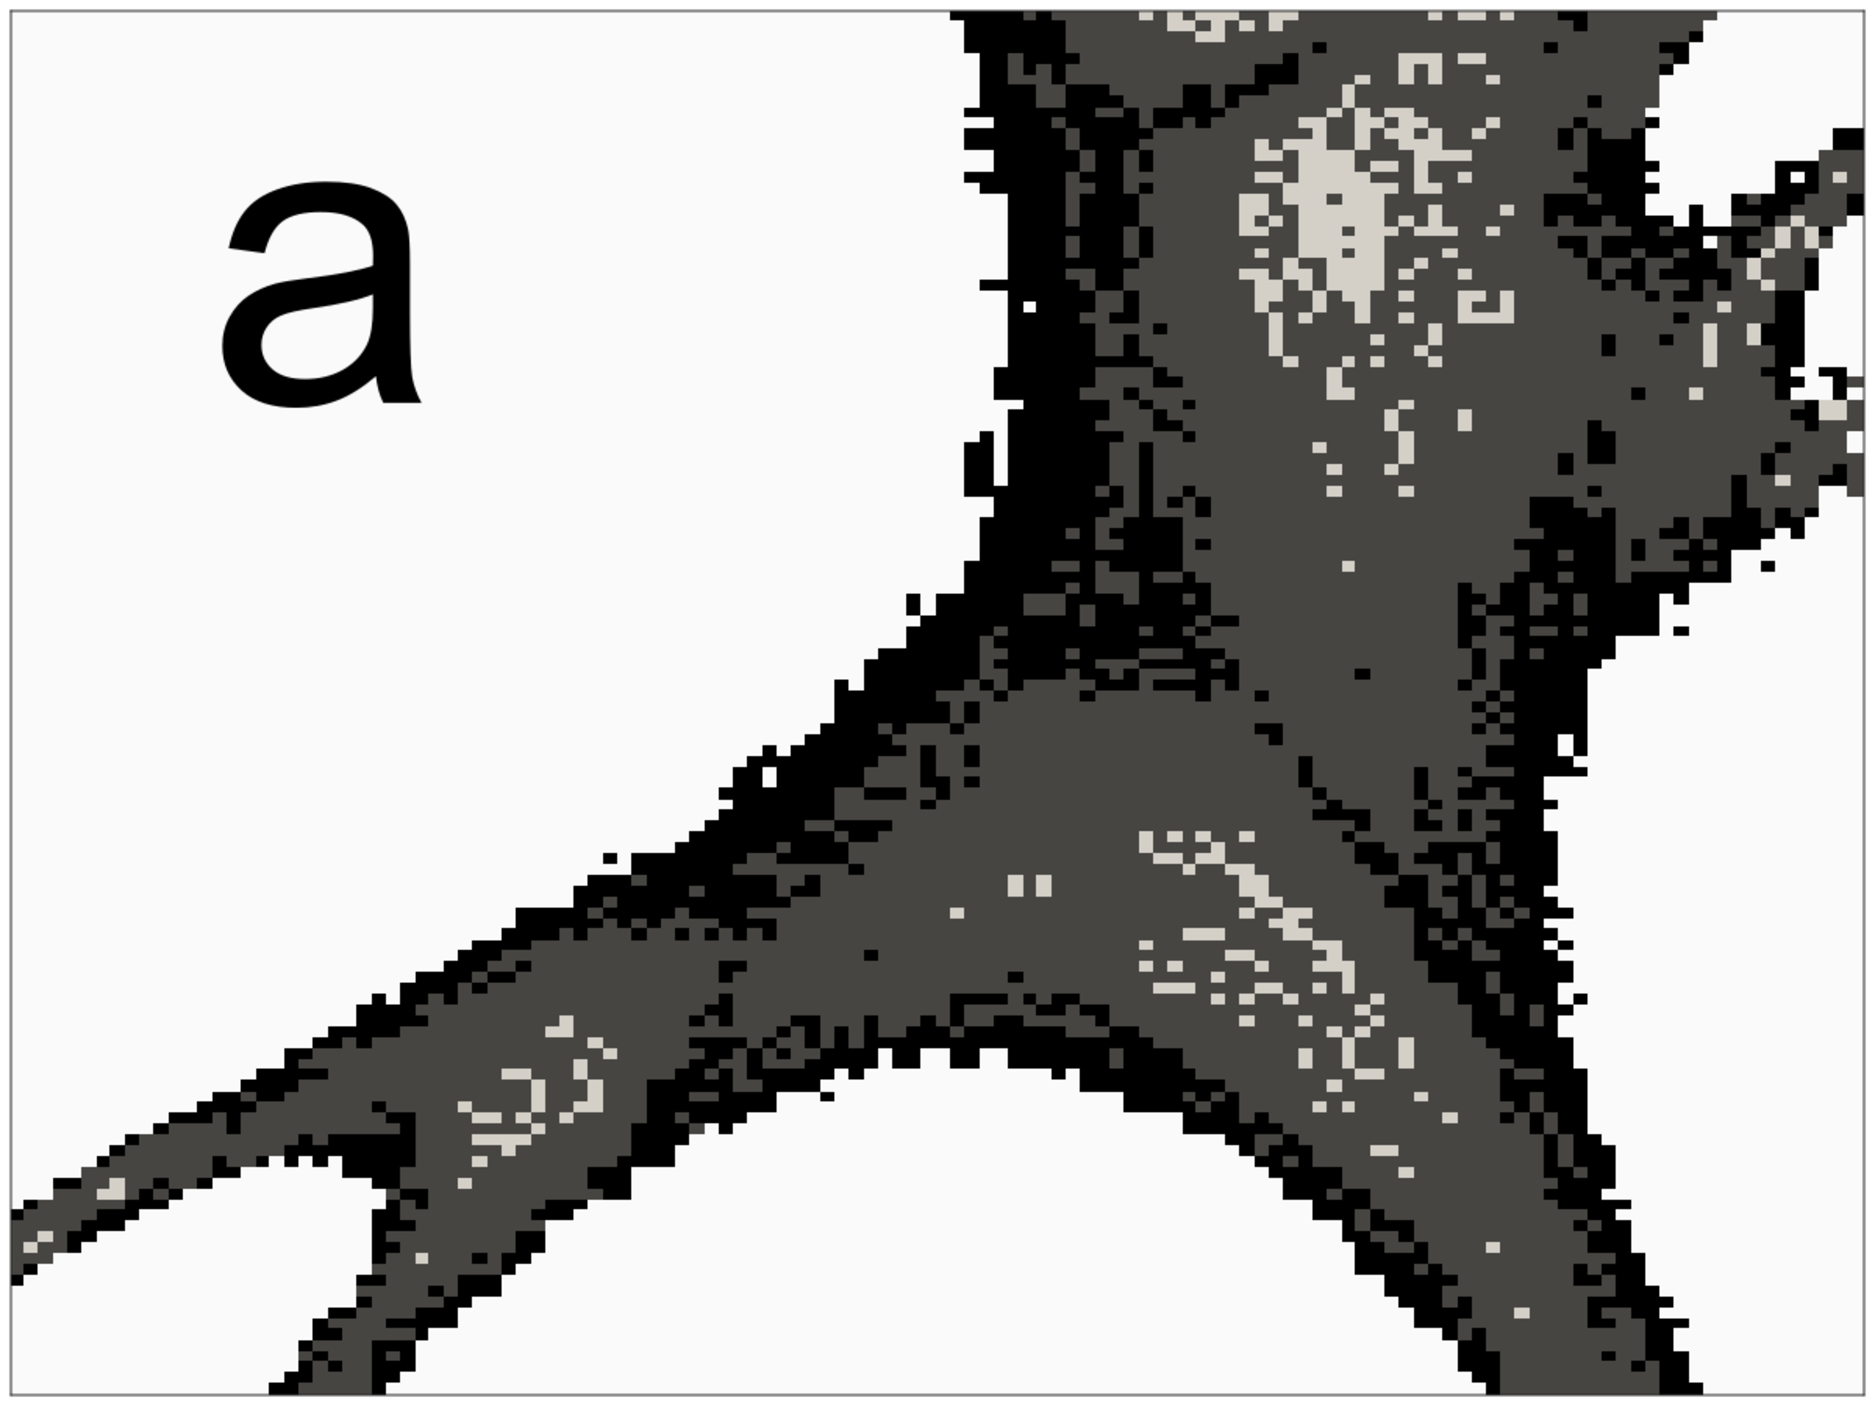
\includegraphics[width=0.35\textwidth]{m5_lu}
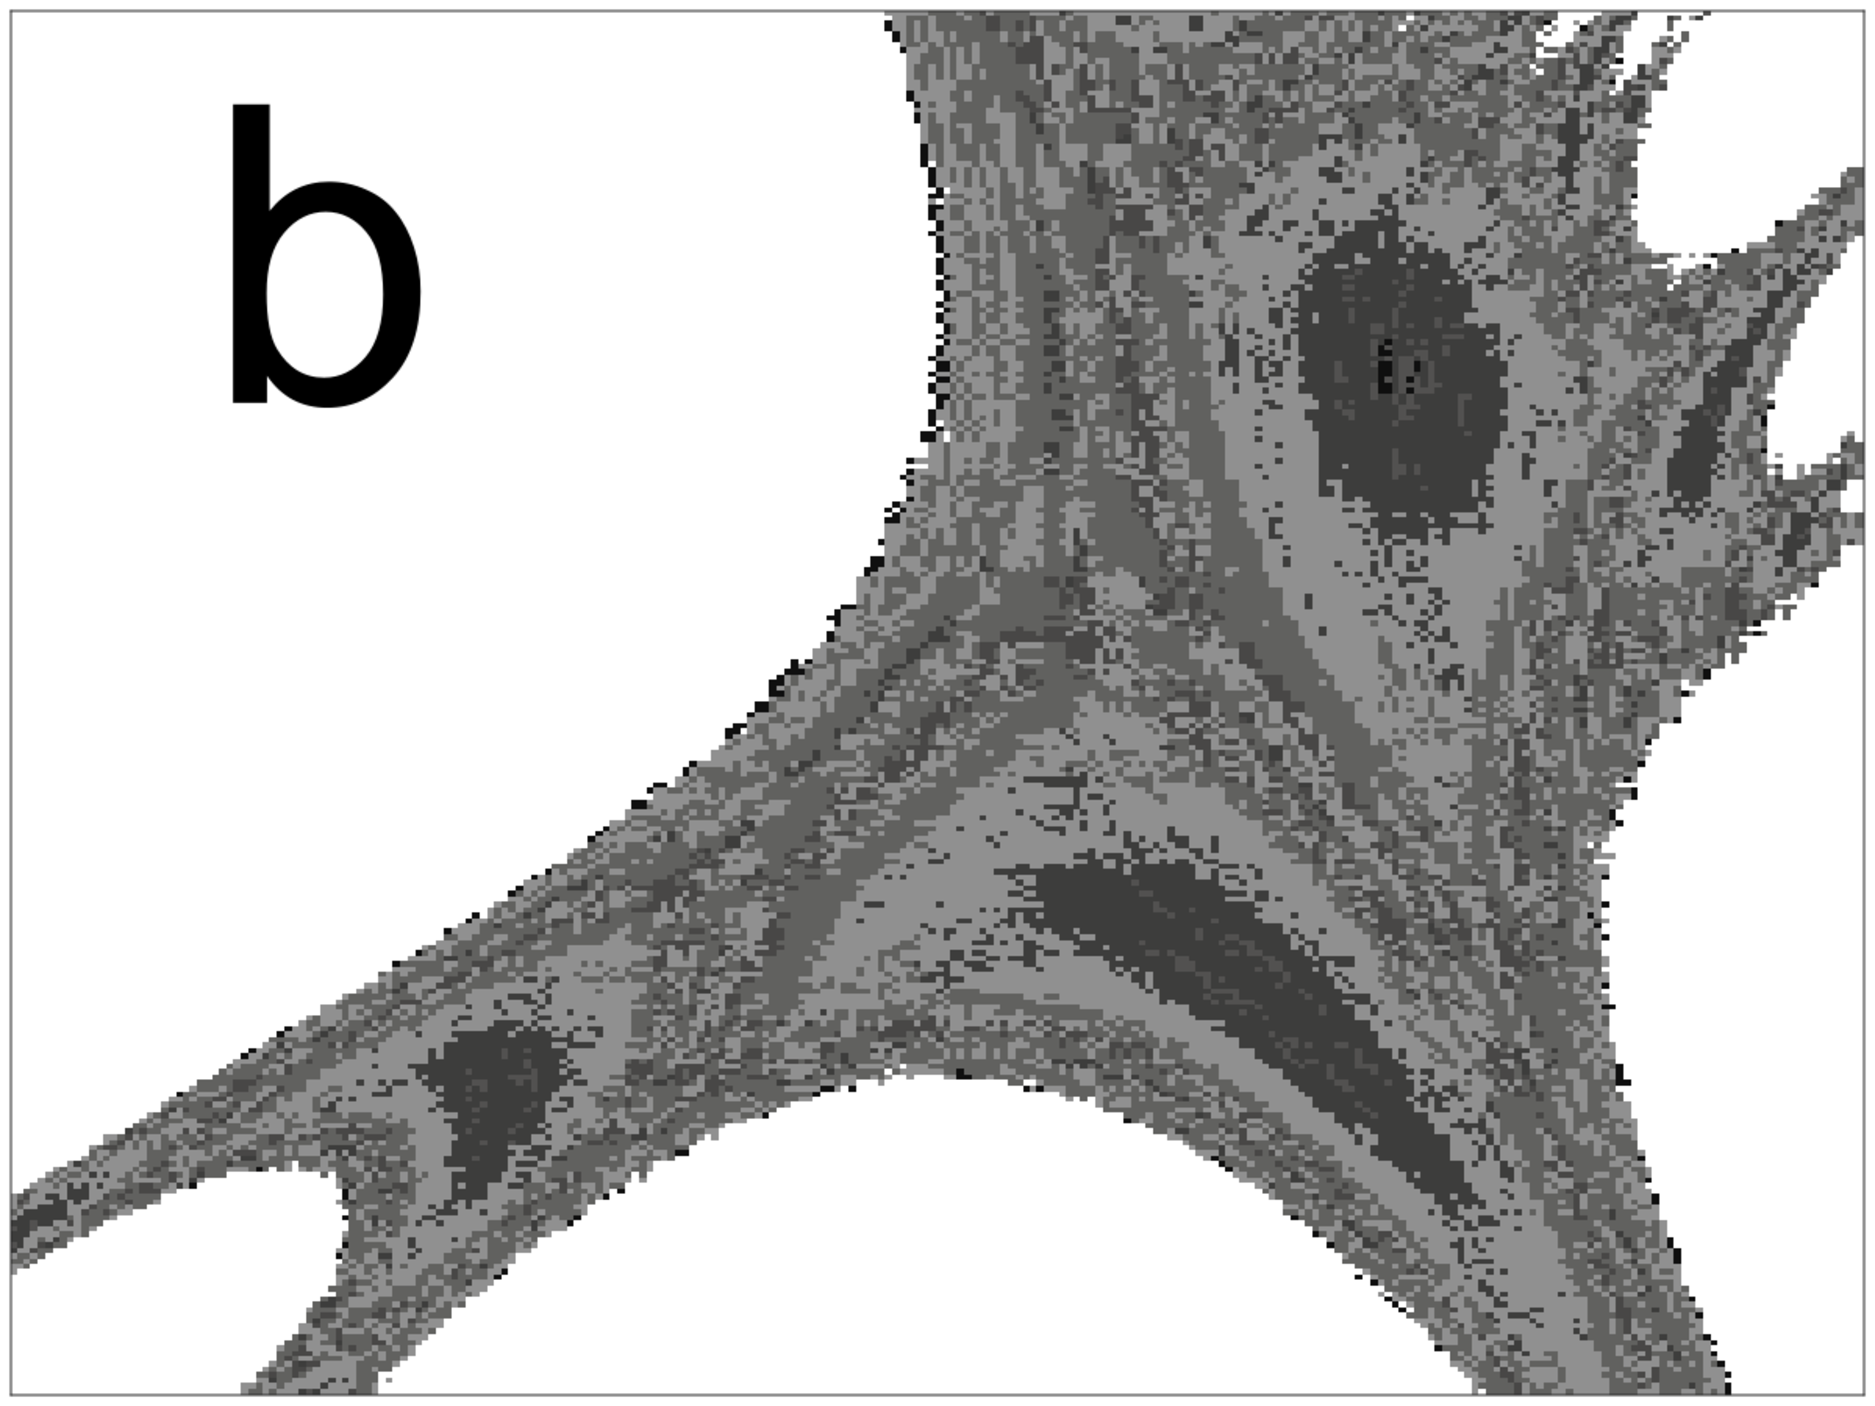
\includegraphics[width=0.35\textwidth]{m6_lu}
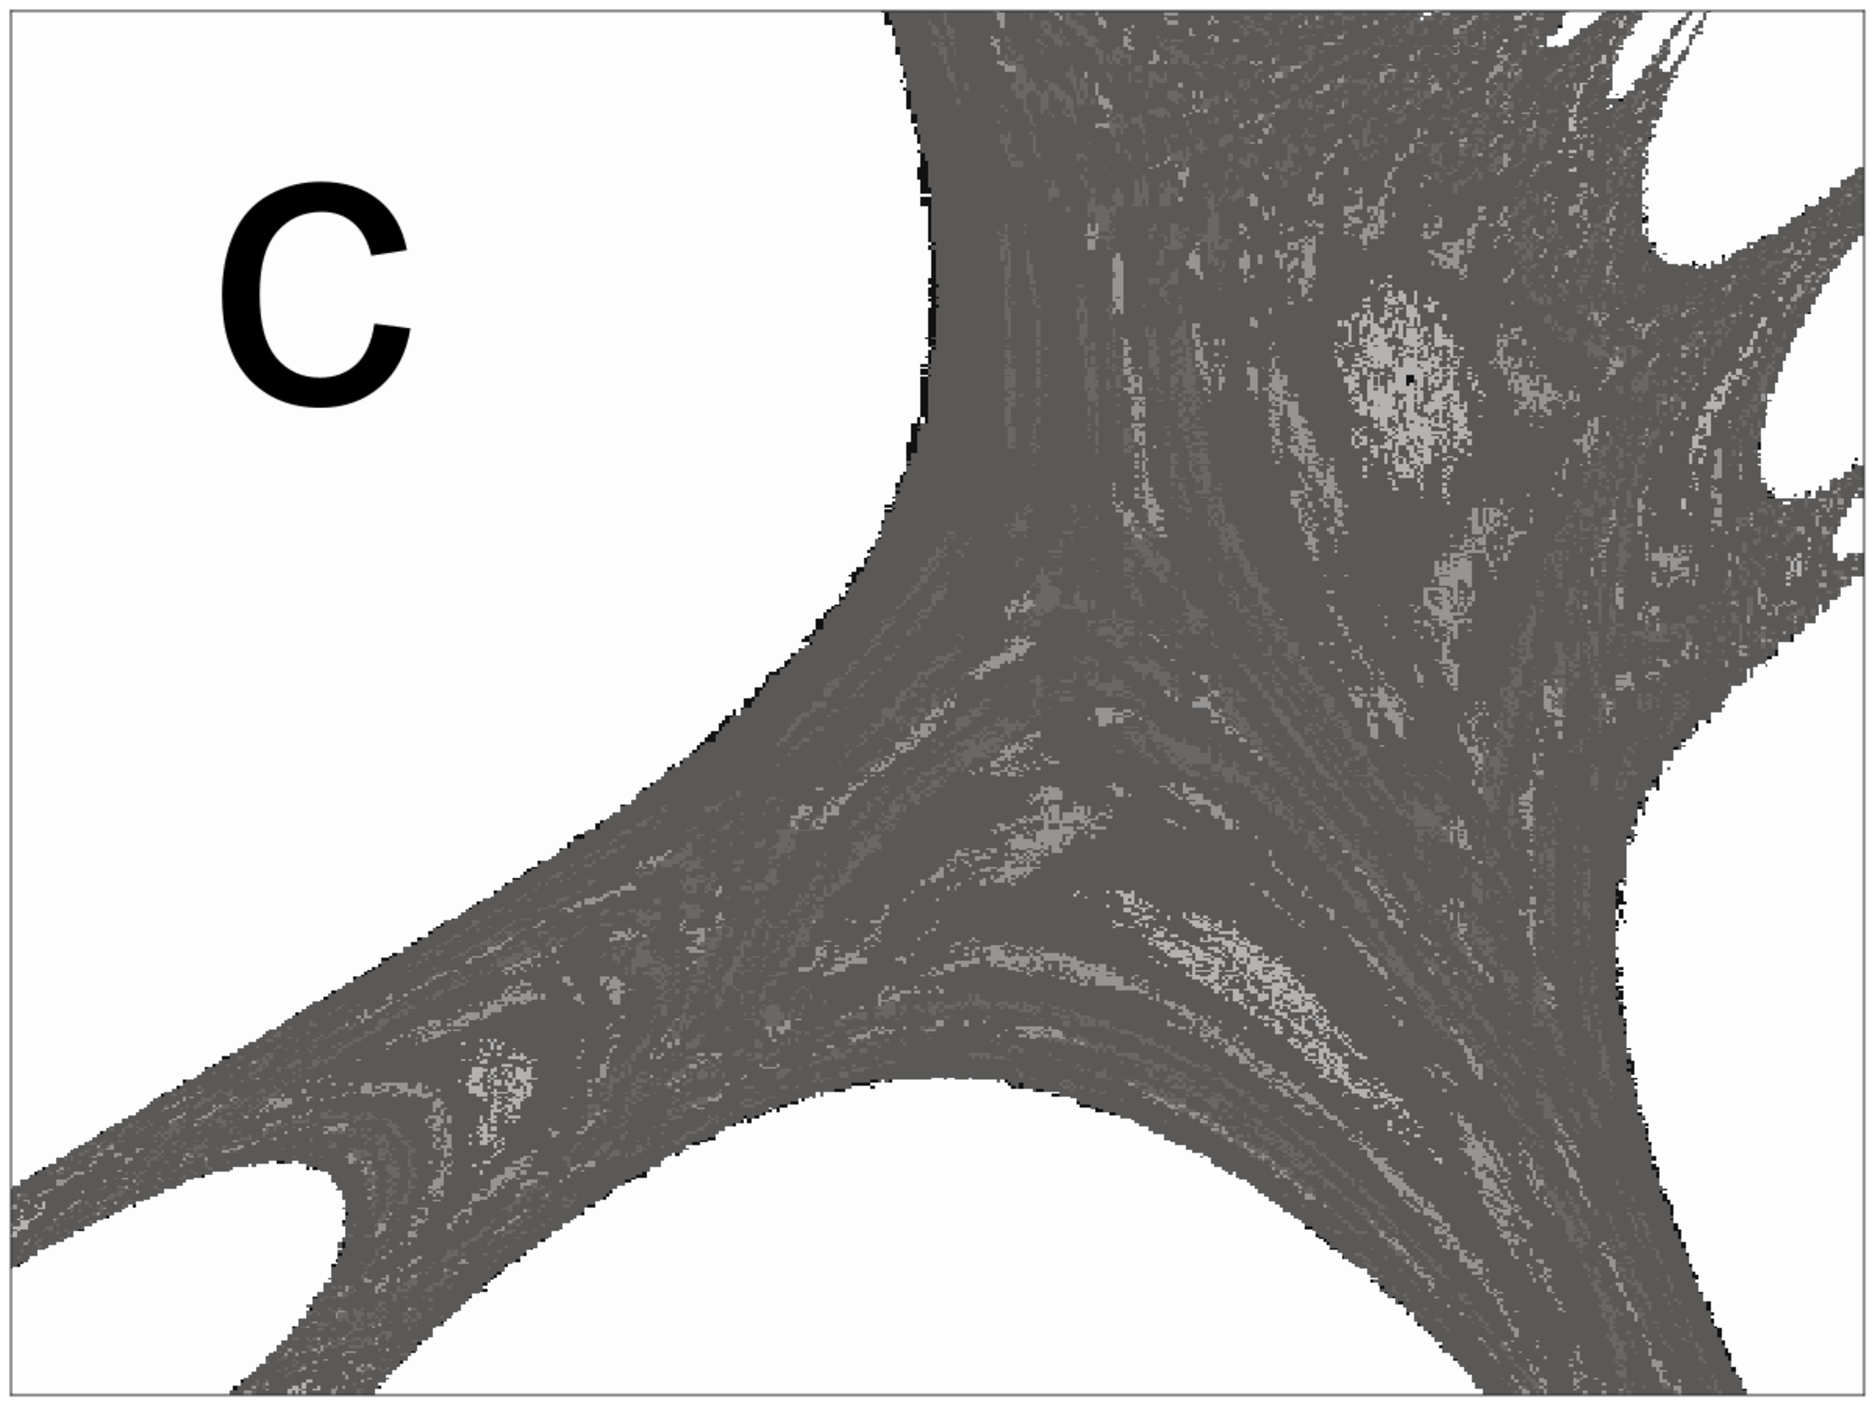
\includegraphics[width=0.35\textwidth]{m7_lu}\\
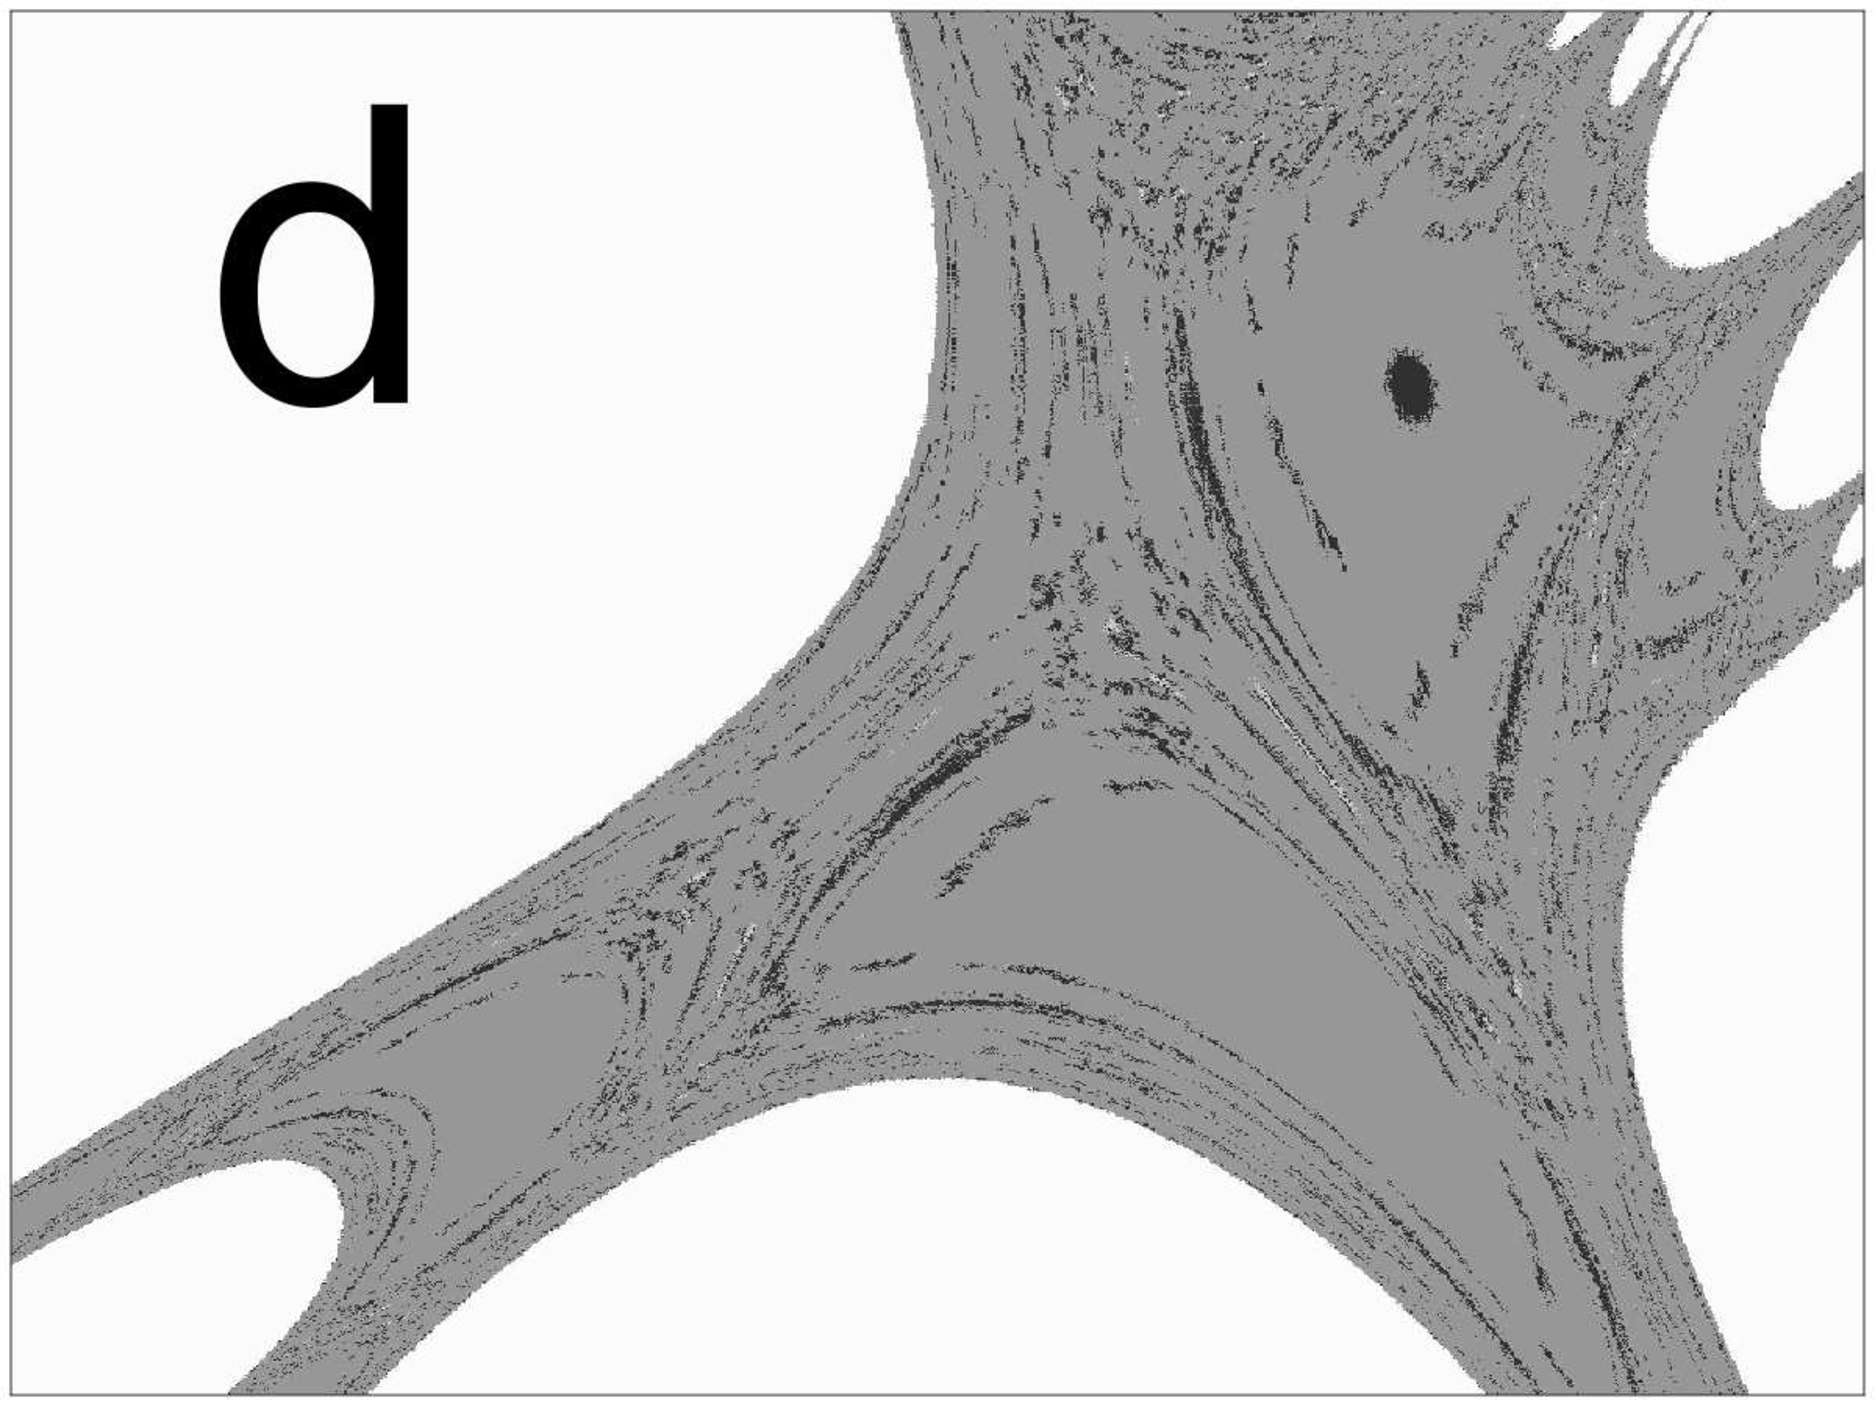
\includegraphics[width=0.35\textwidth]{m8_lu}
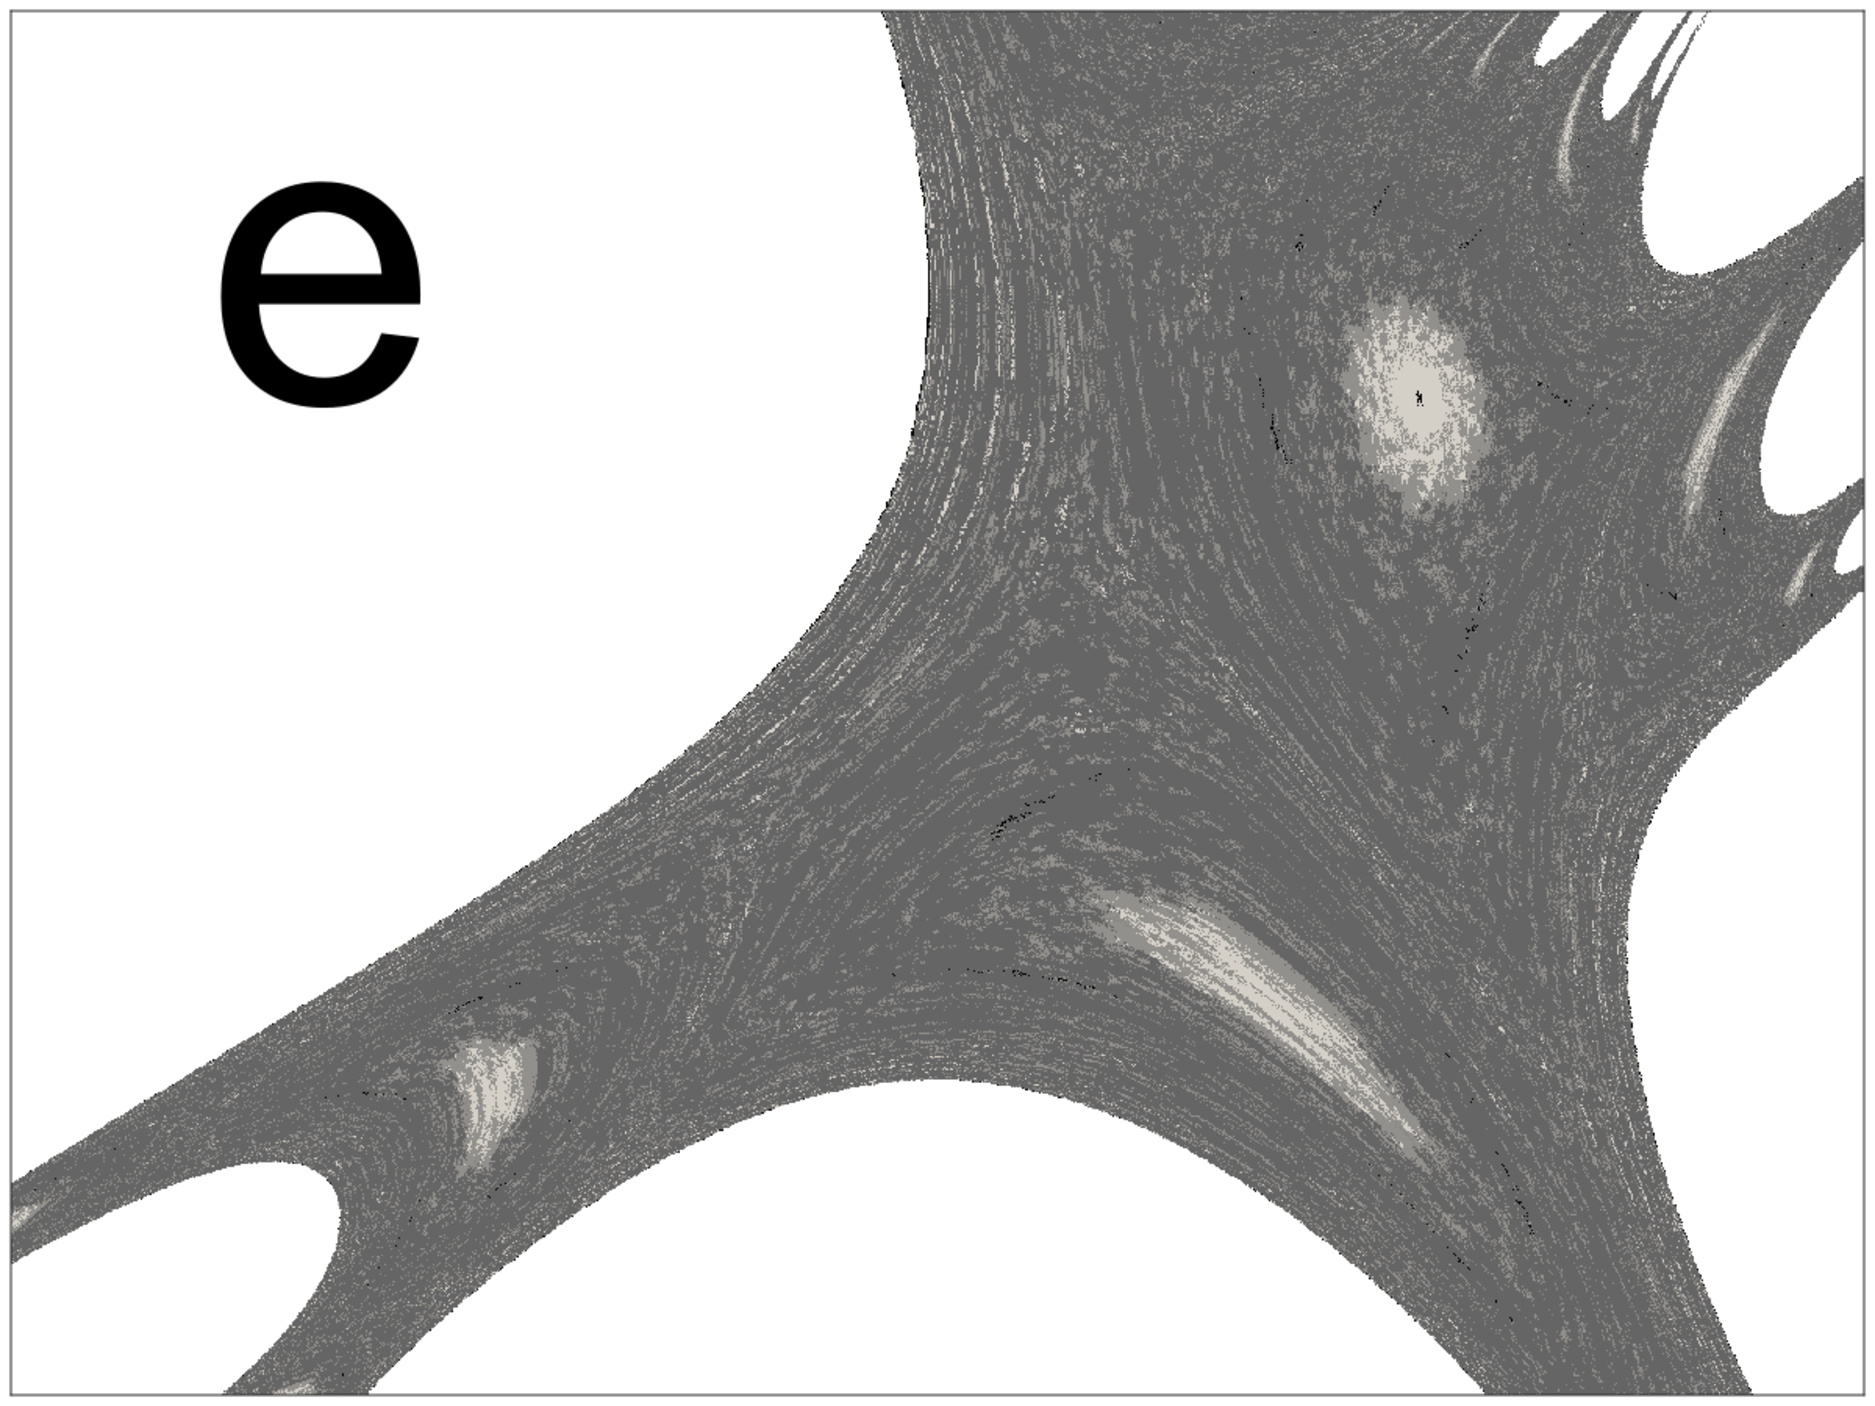
\includegraphics[width=0.35\textwidth]{m9_lu}
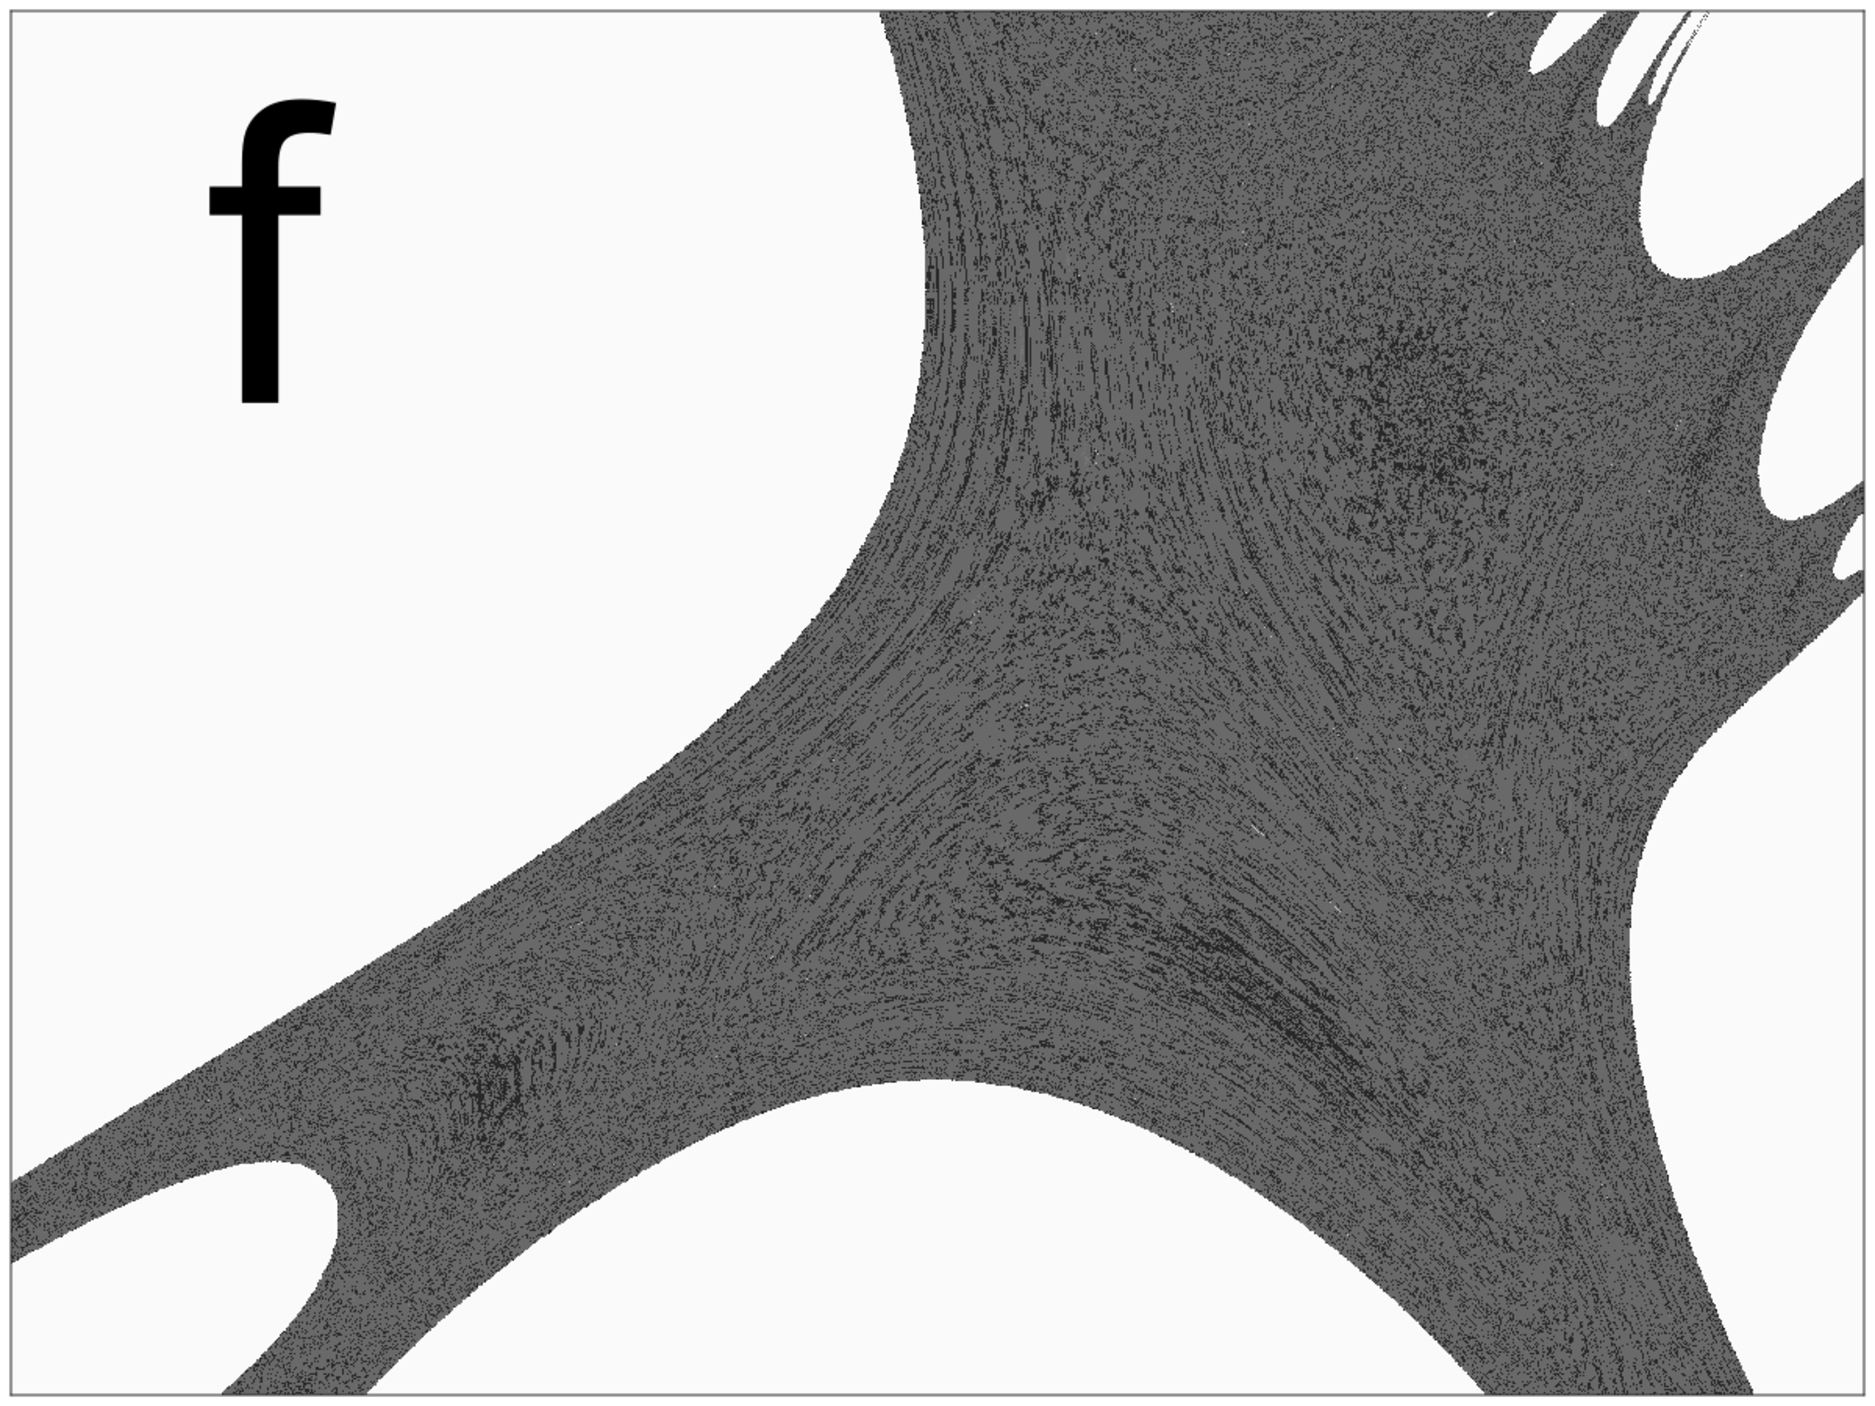
\includegraphics[width=0.35\textwidth]{m10_lu}\\
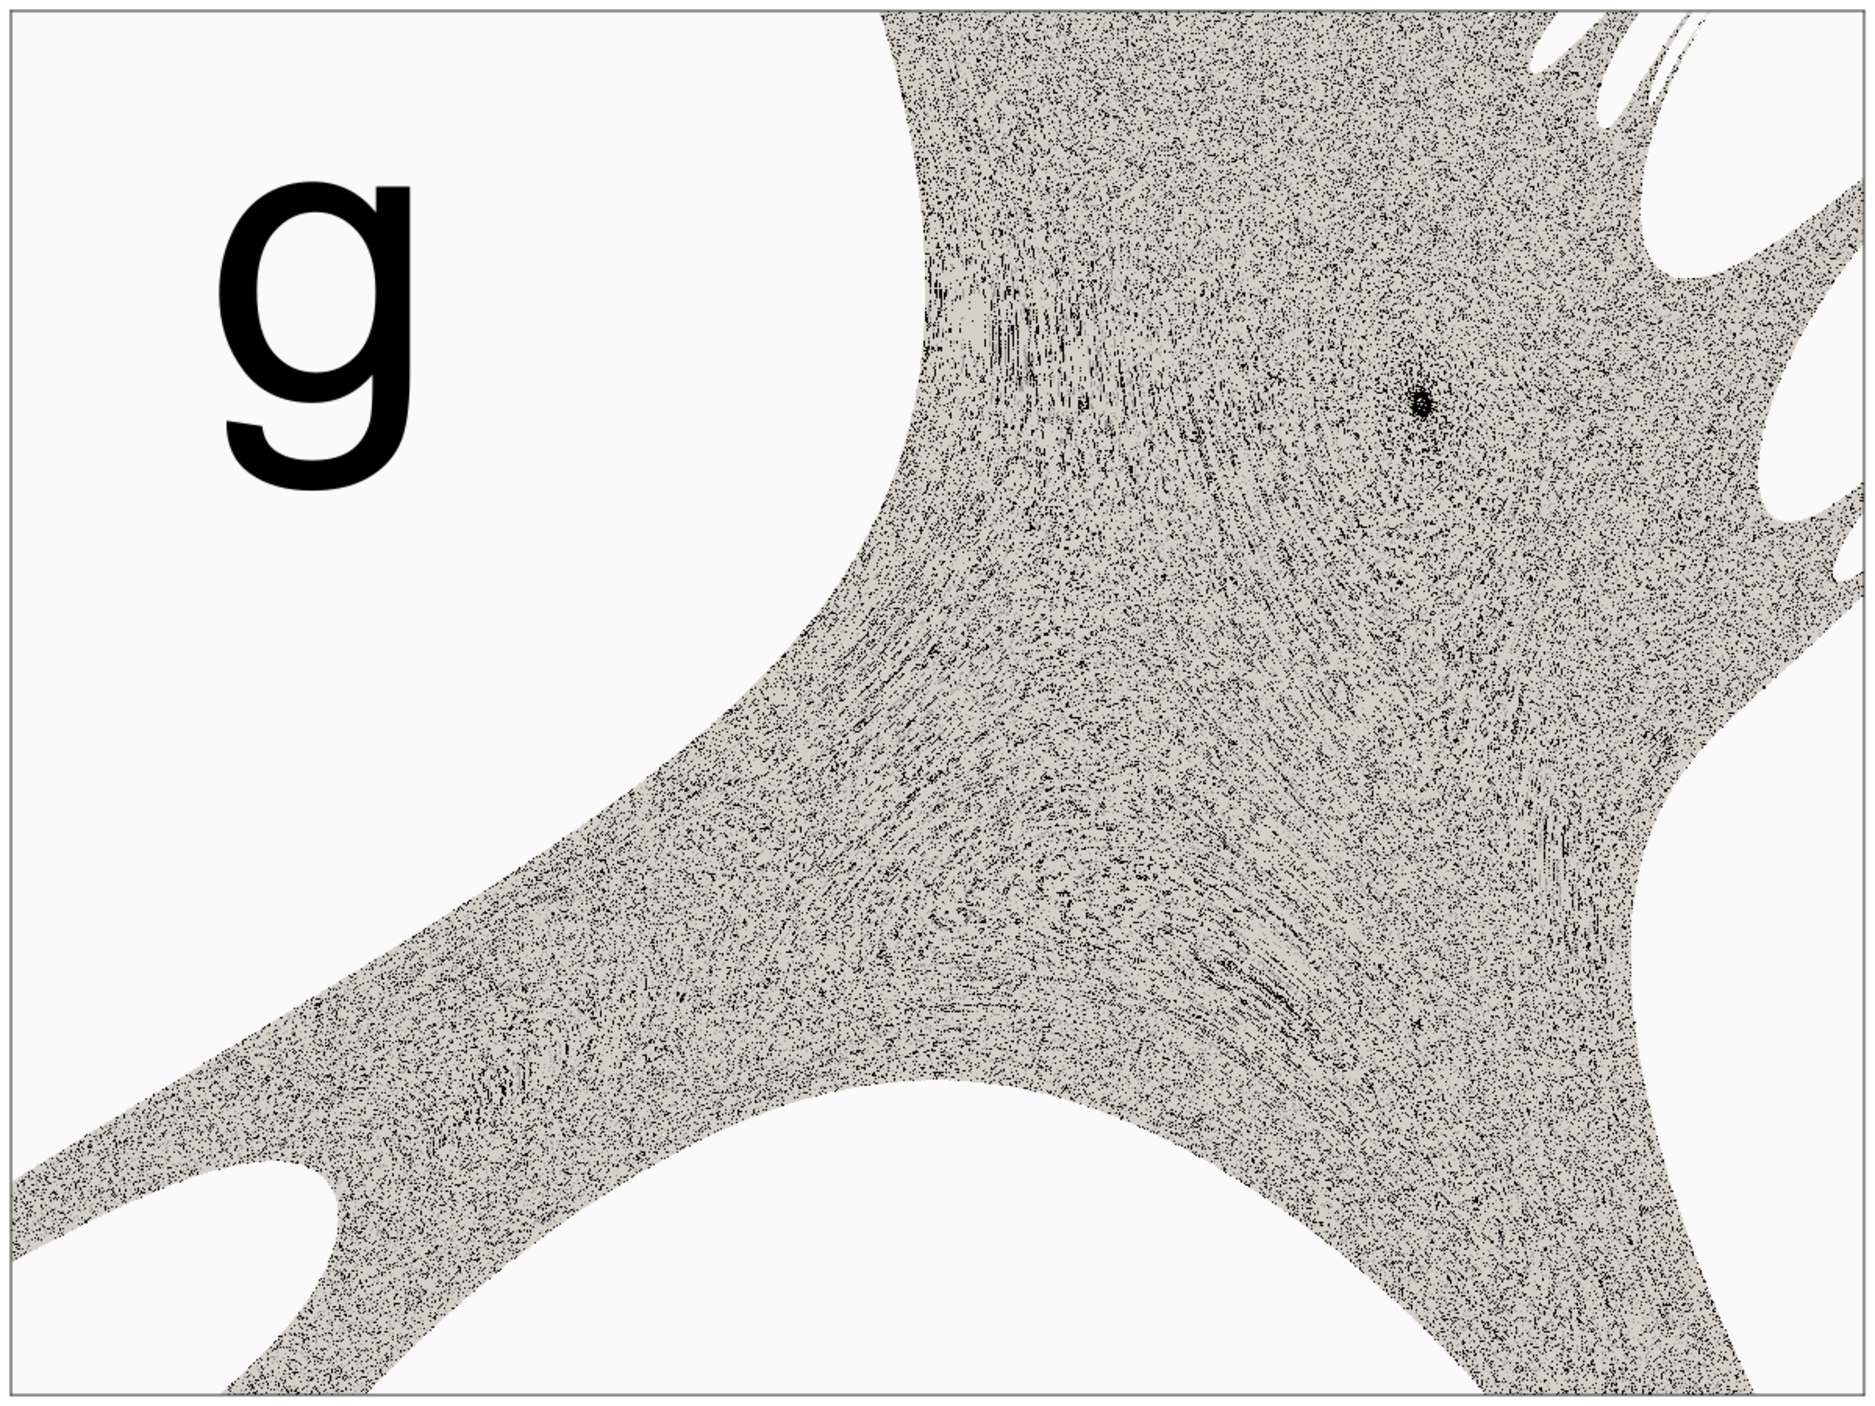
\includegraphics[width=0.35\textwidth]{m11_lu}
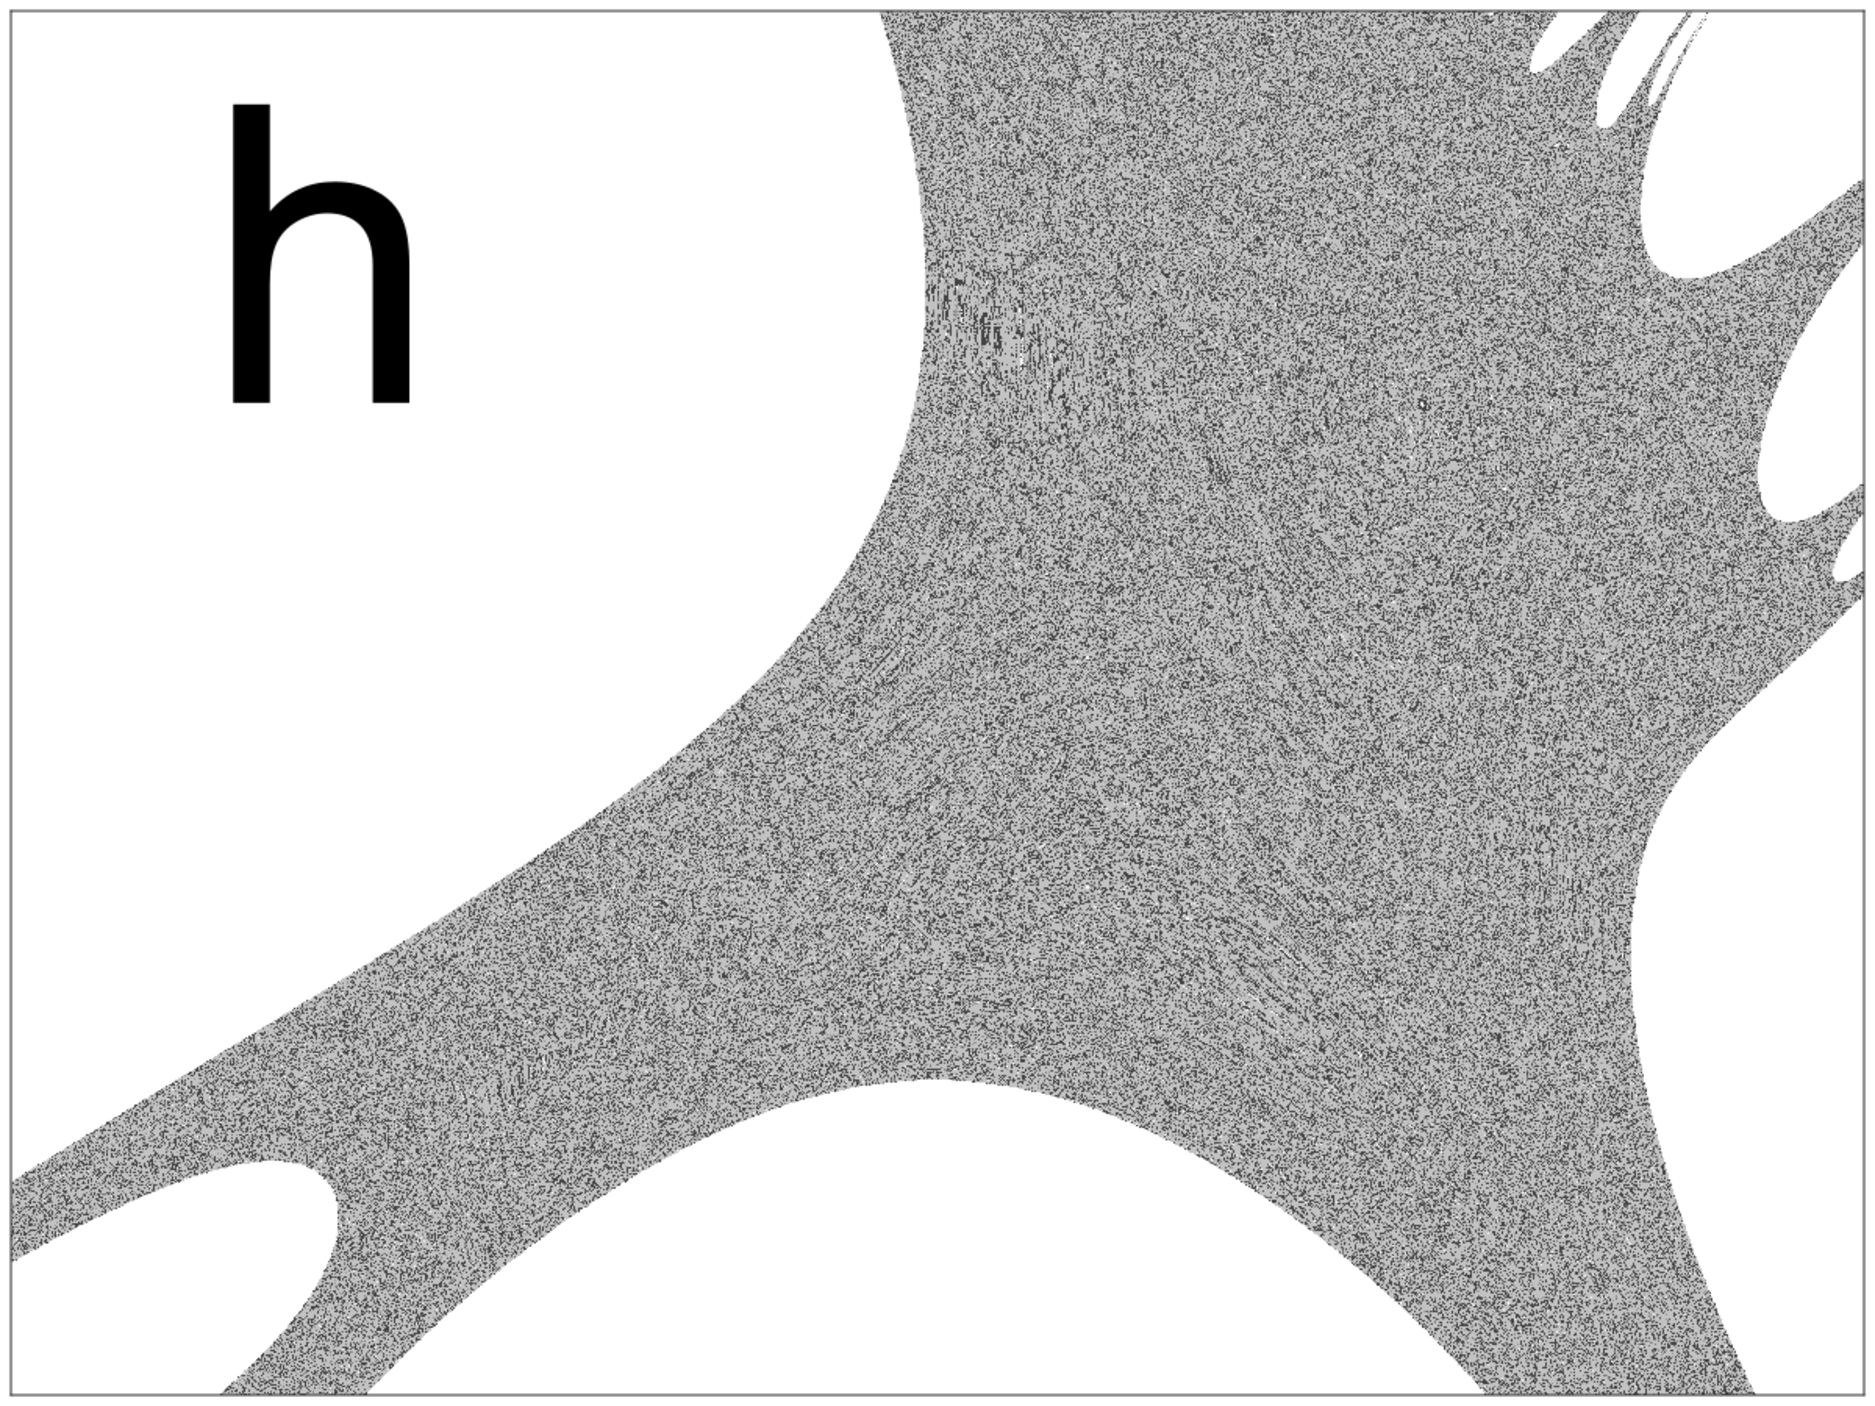
\includegraphics[width=0.35\textwidth]{m12_lu}
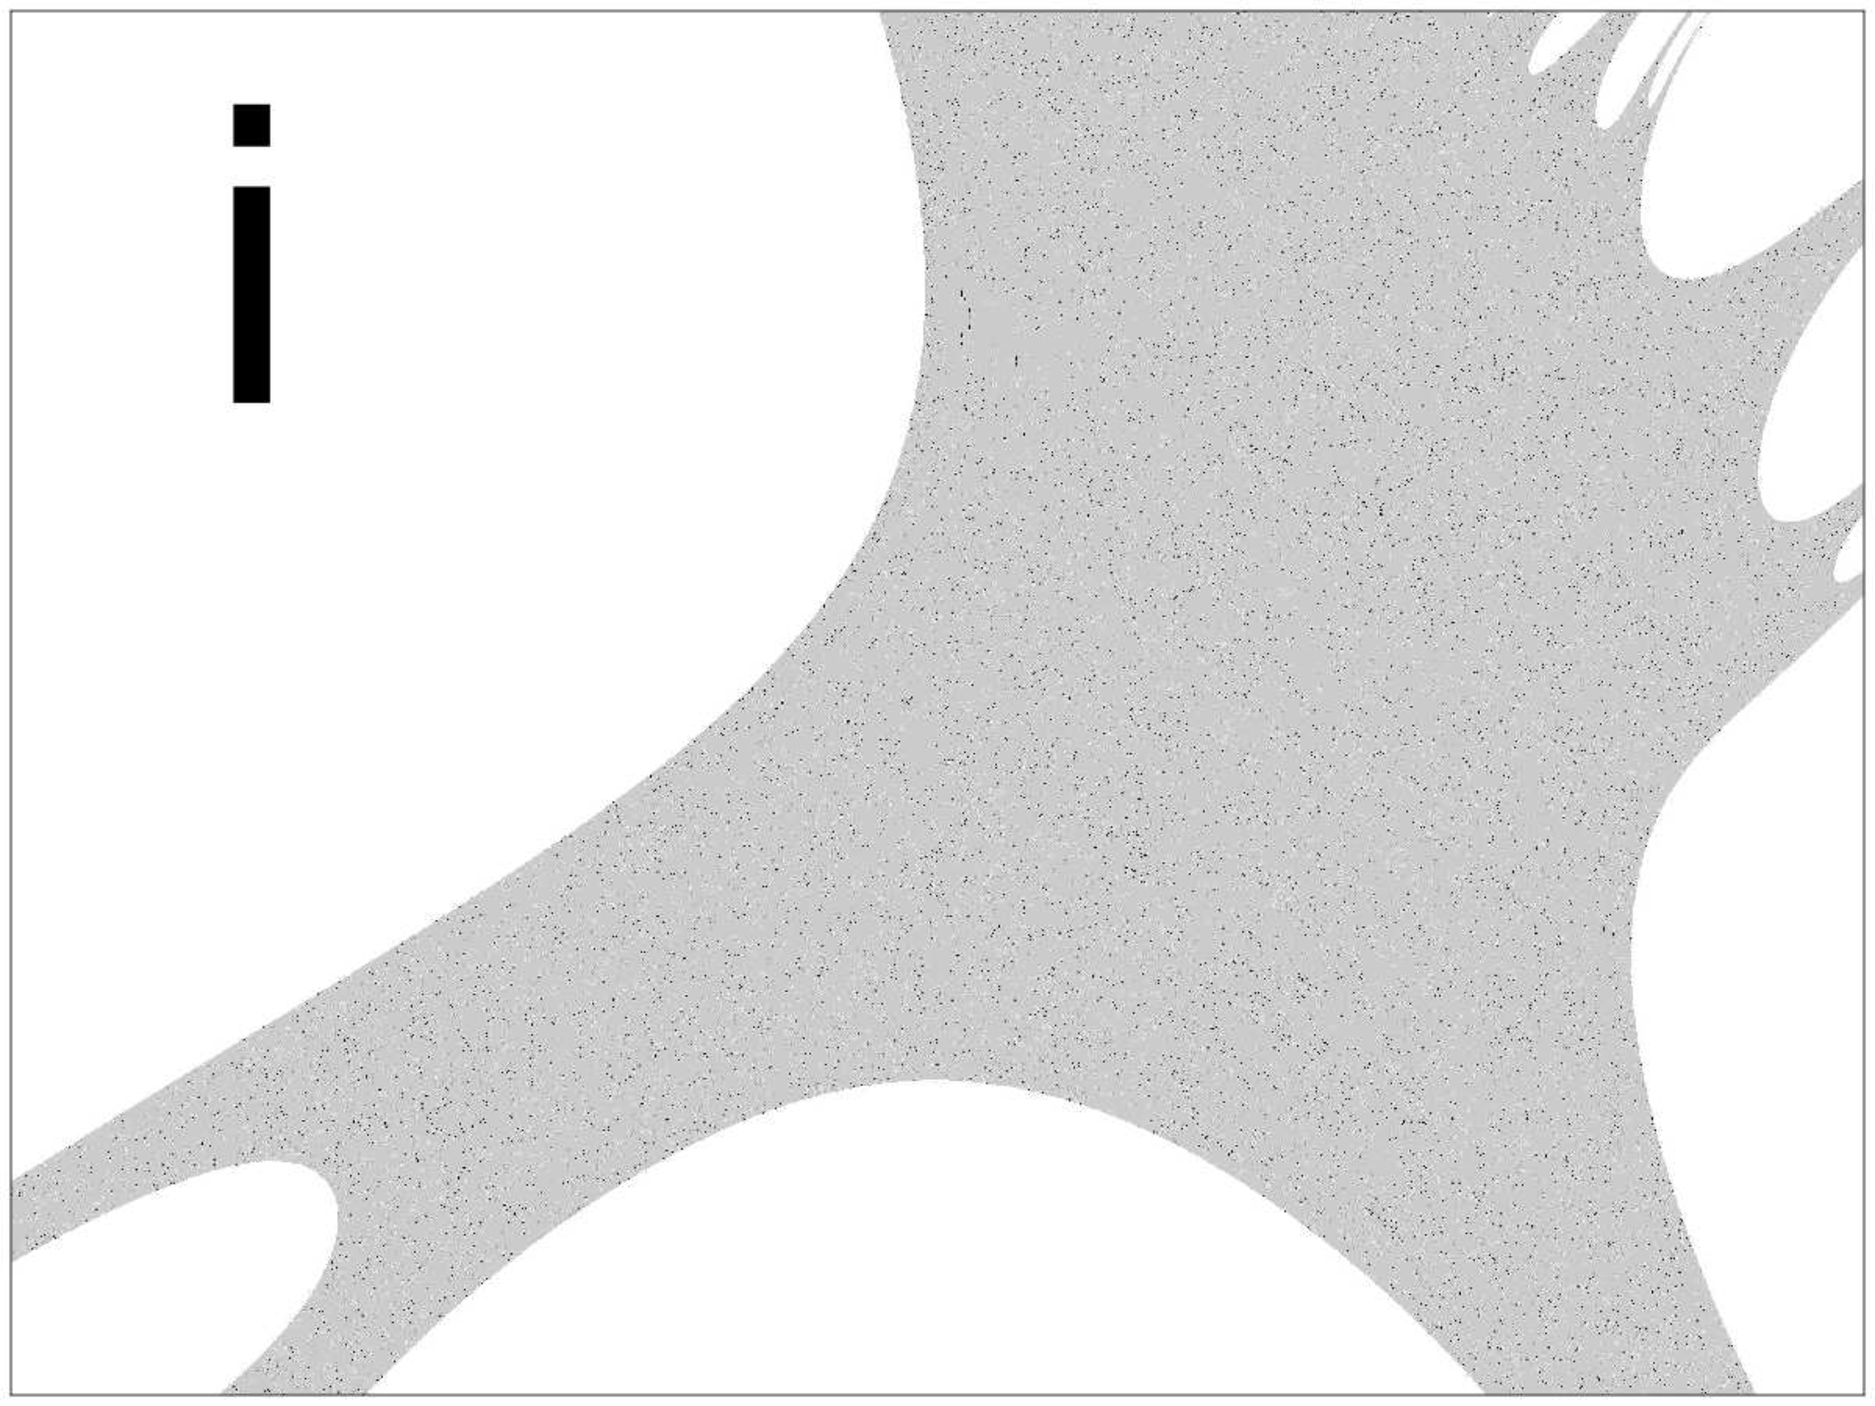
\includegraphics[width=0.35\textwidth]{m13_lu}\\
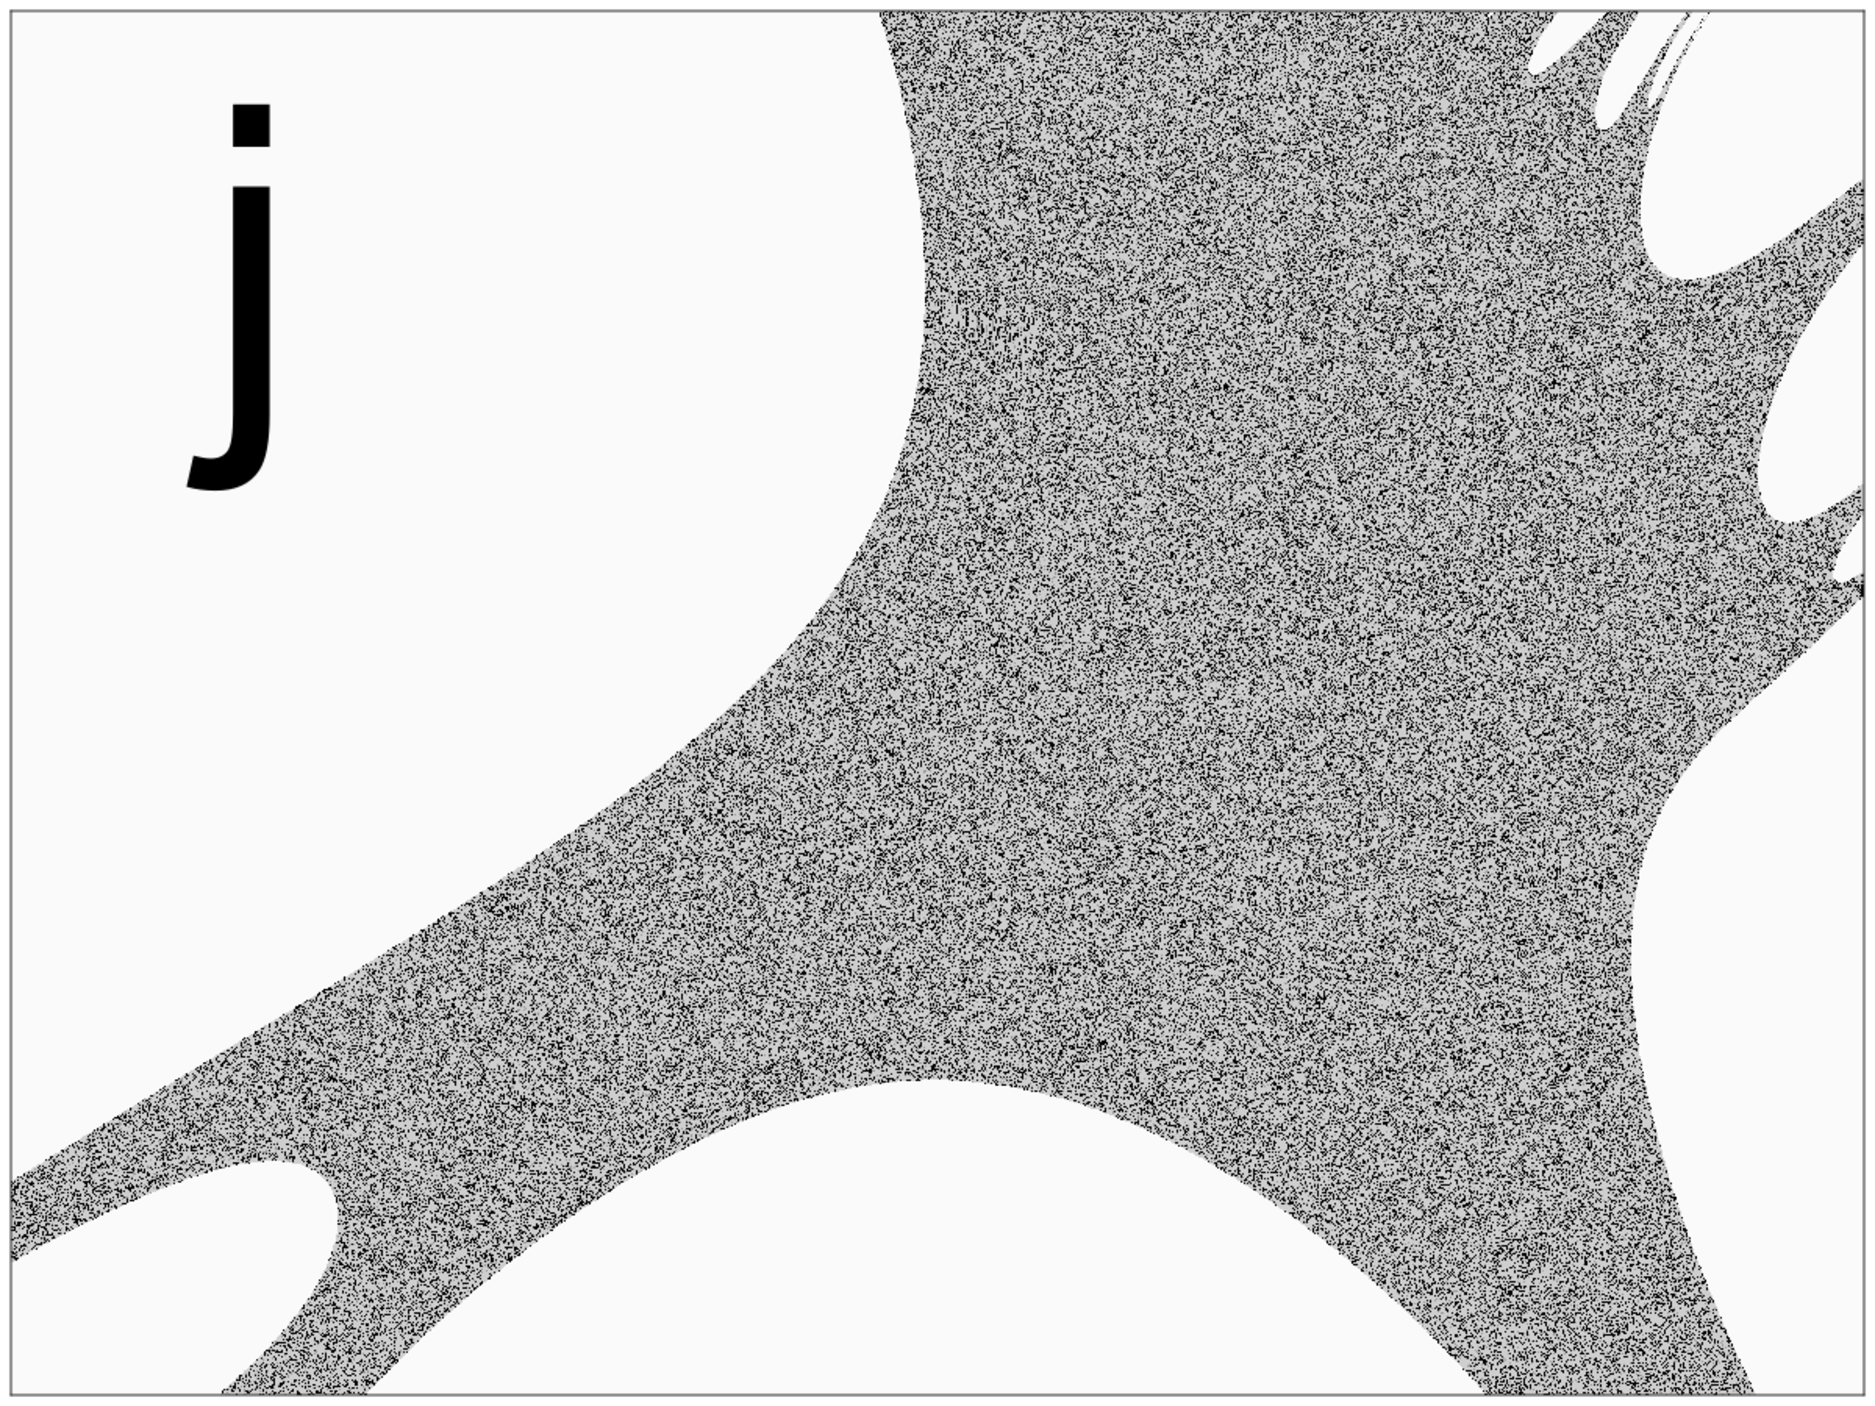
\includegraphics[width=0.35\textwidth]{m14_lu}
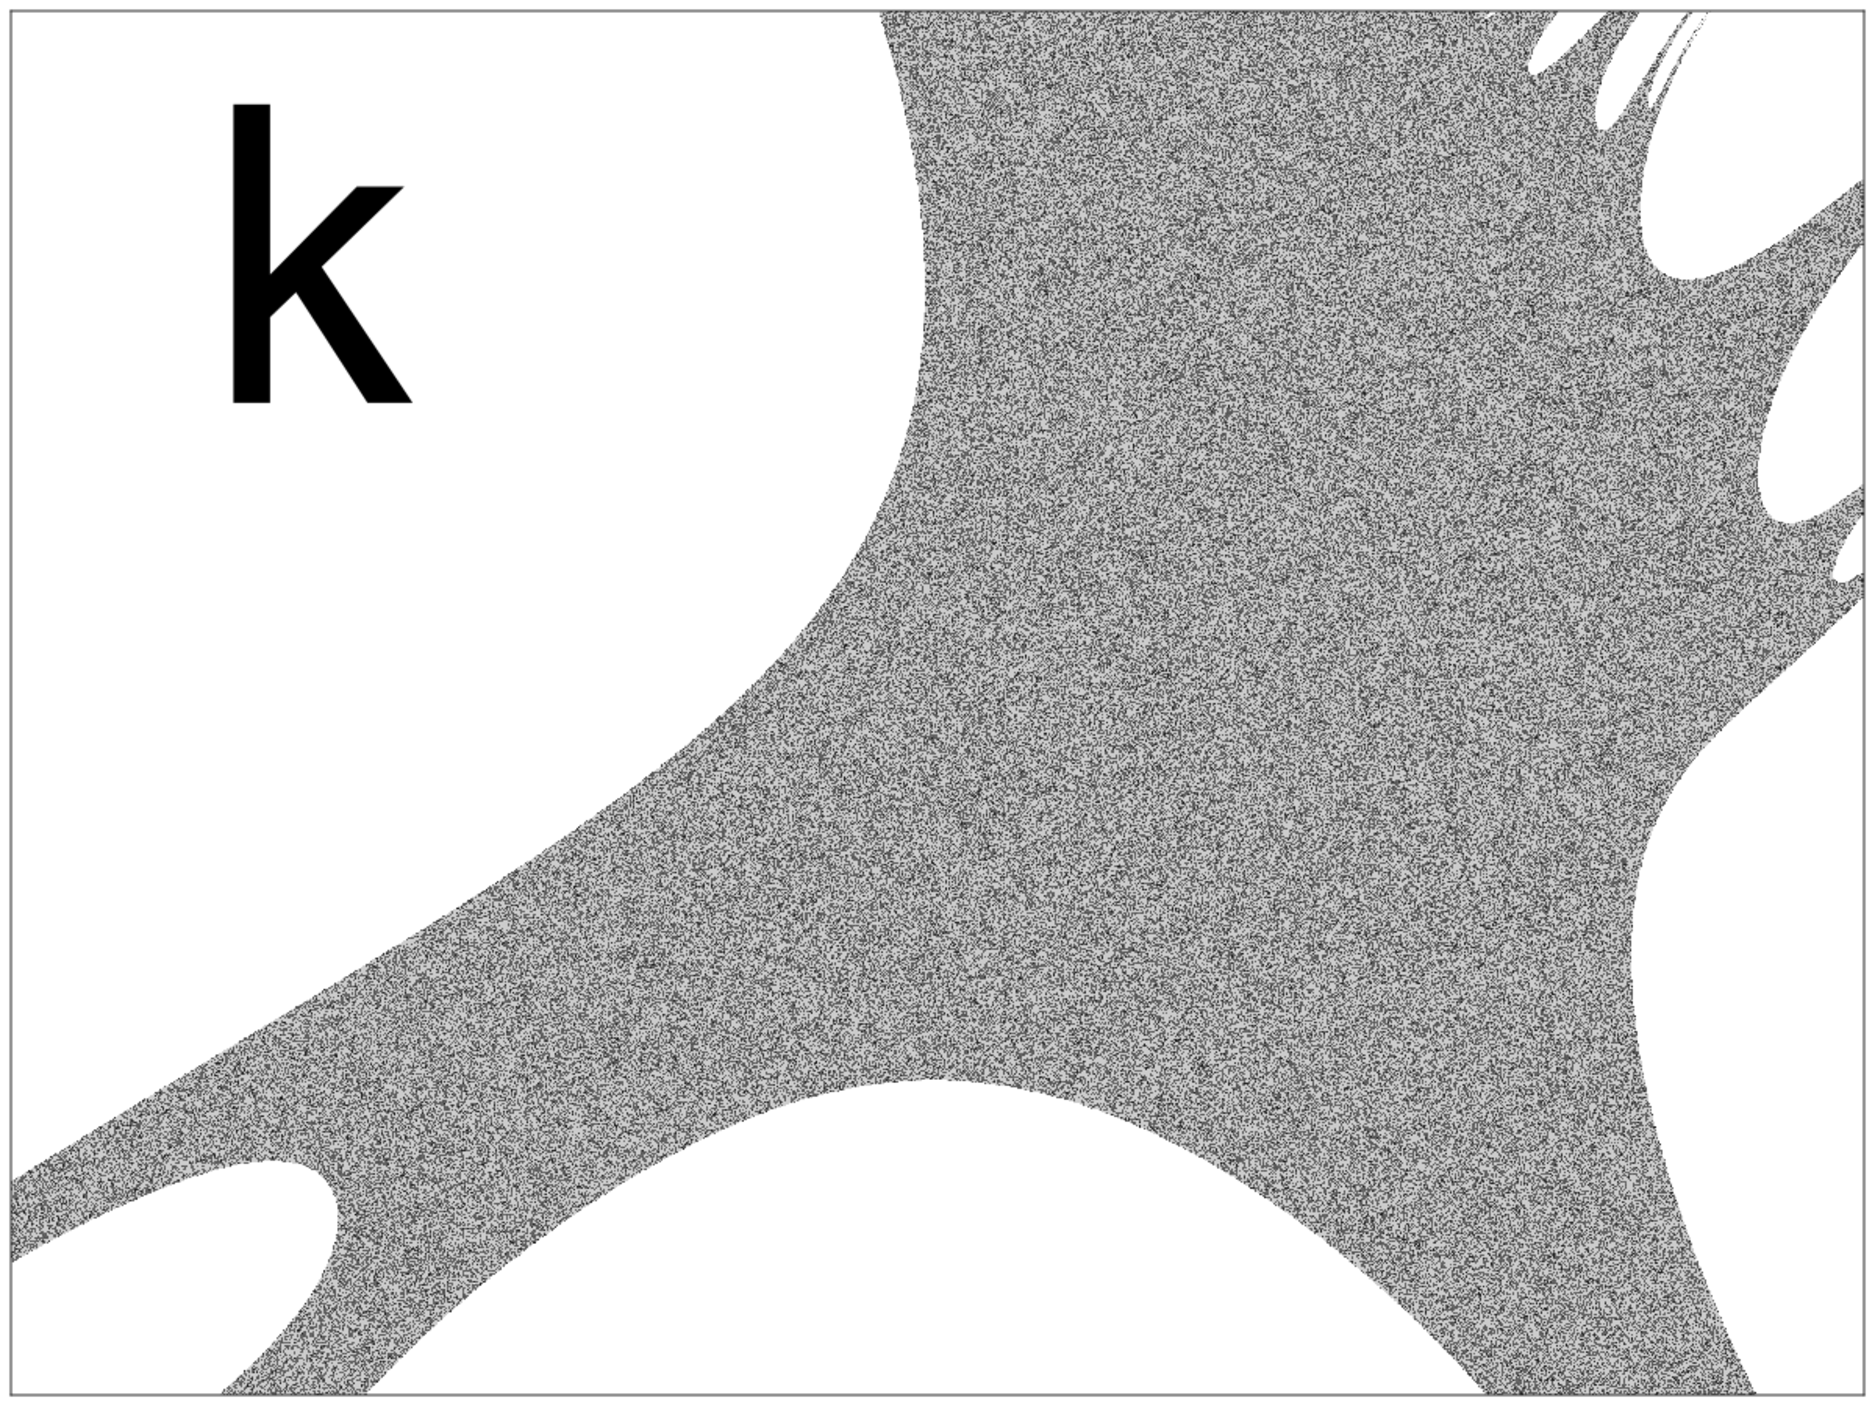
\includegraphics[width=0.35\textwidth]{m17_lu}
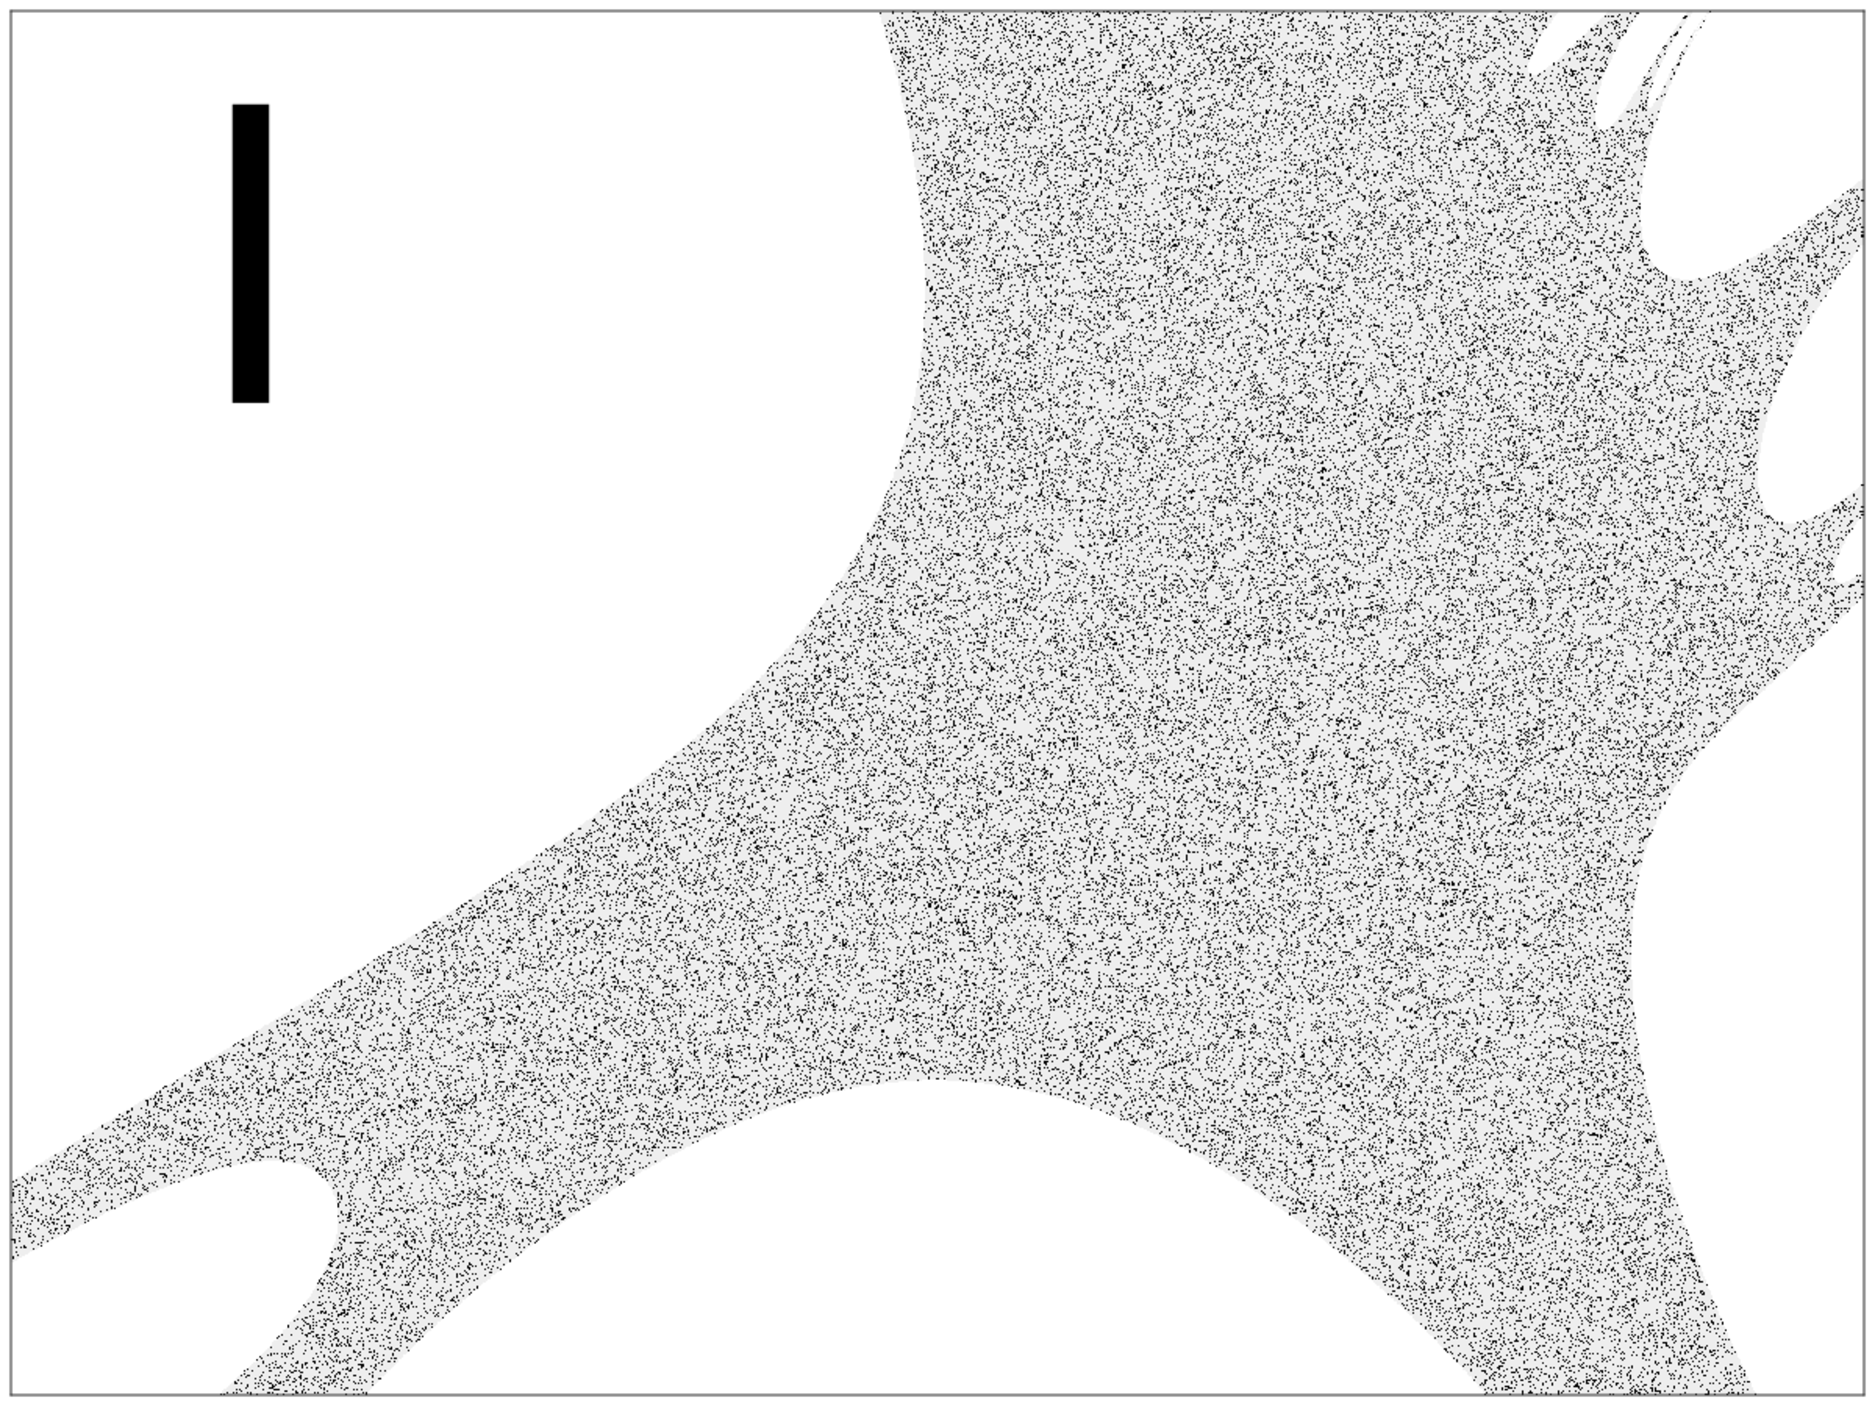
\includegraphics[width=0.35\textwidth]{m18_lu}\\
\end{tabular}
\caption{Coexisting areas in attraction domains for: (a) $n_f=5$, (b) $n_f=6$, (c) $n_f=7$, (d) $n_f=8$, (e) $n_f=9$, (f) $n_f=10$, (g) $n_f=11$, (h) $n_f=12$, (i) $n_f=13$, (j) $n_f=14$, (k) $n_f=17$, (l) $n_f=18$.}
\label{fig:avvelo}
\end{figure*}

With the purpose of being able to distinguish the different coexisting areas, a diverse range of gray tones have been used on each figure.
It must be taken into account that each figure has its own gray range, this means that, for example, an almost white area when $n_f = 5$ (Fig. \ref{fig:avvelo}.a) corresponds to a period of $6$, while a darker area in a figure with higher $n_f$ may correspond to a period higher than a thousand (Fig. \ref{fig:avvelo}.e).
These figures allow reflecting the  complex domains of attraction that appear when digitalizing.

It can be seen in Fig. \ref{fig:avvelo} that the smaller the value of $n_f$ the bigger the area of ICs that tends to diverge and to converge to fixed points.
As $n_f$ increases, the area of divergent and fixed points decreases.
These figures along with Table \ref{tabla} allows an easy interpretation of the system's behavior.
In Table \ref{tabla} the sequence lengths that appear in the attractor domain for every $n_f$ are sorted by the more to the less numerous ICs that converges to that cycle.
It can be seen the rate of occurrence.
Indeed, figures with lower values of $n_f$ present irregular, or rough surfaces, pointing out that different lengths cycles coexist there.
For example, for $n_f=5$ there is a prevalence of  short periods cycles.
In that case, there exist just two limit cycles, the lighter grey zone corresponds to the attraction domain of the limit cycles of length six, that is the less numerous cycle, according to Table \ref{tabla}, and, the darker zone corresponds to the attraction domain of length two cycle.

Although for $n_f \geqslant 13$ (Figures \ref{fig:avvelo}.i to \ref{fig:avvelo}.l) the attractor domain appears to be smooth and uniform, however, if we enlarge a section of the figures (Fig. \ref{fig:m_zoom}) it can be seen that there are still cycles with different periods that coexist in the attractor for $n_f=14$,$17$ and $18$.
%
\begin{figure}
    \centering
    \begin{subfigure}[t]{0.49\textwidth}
        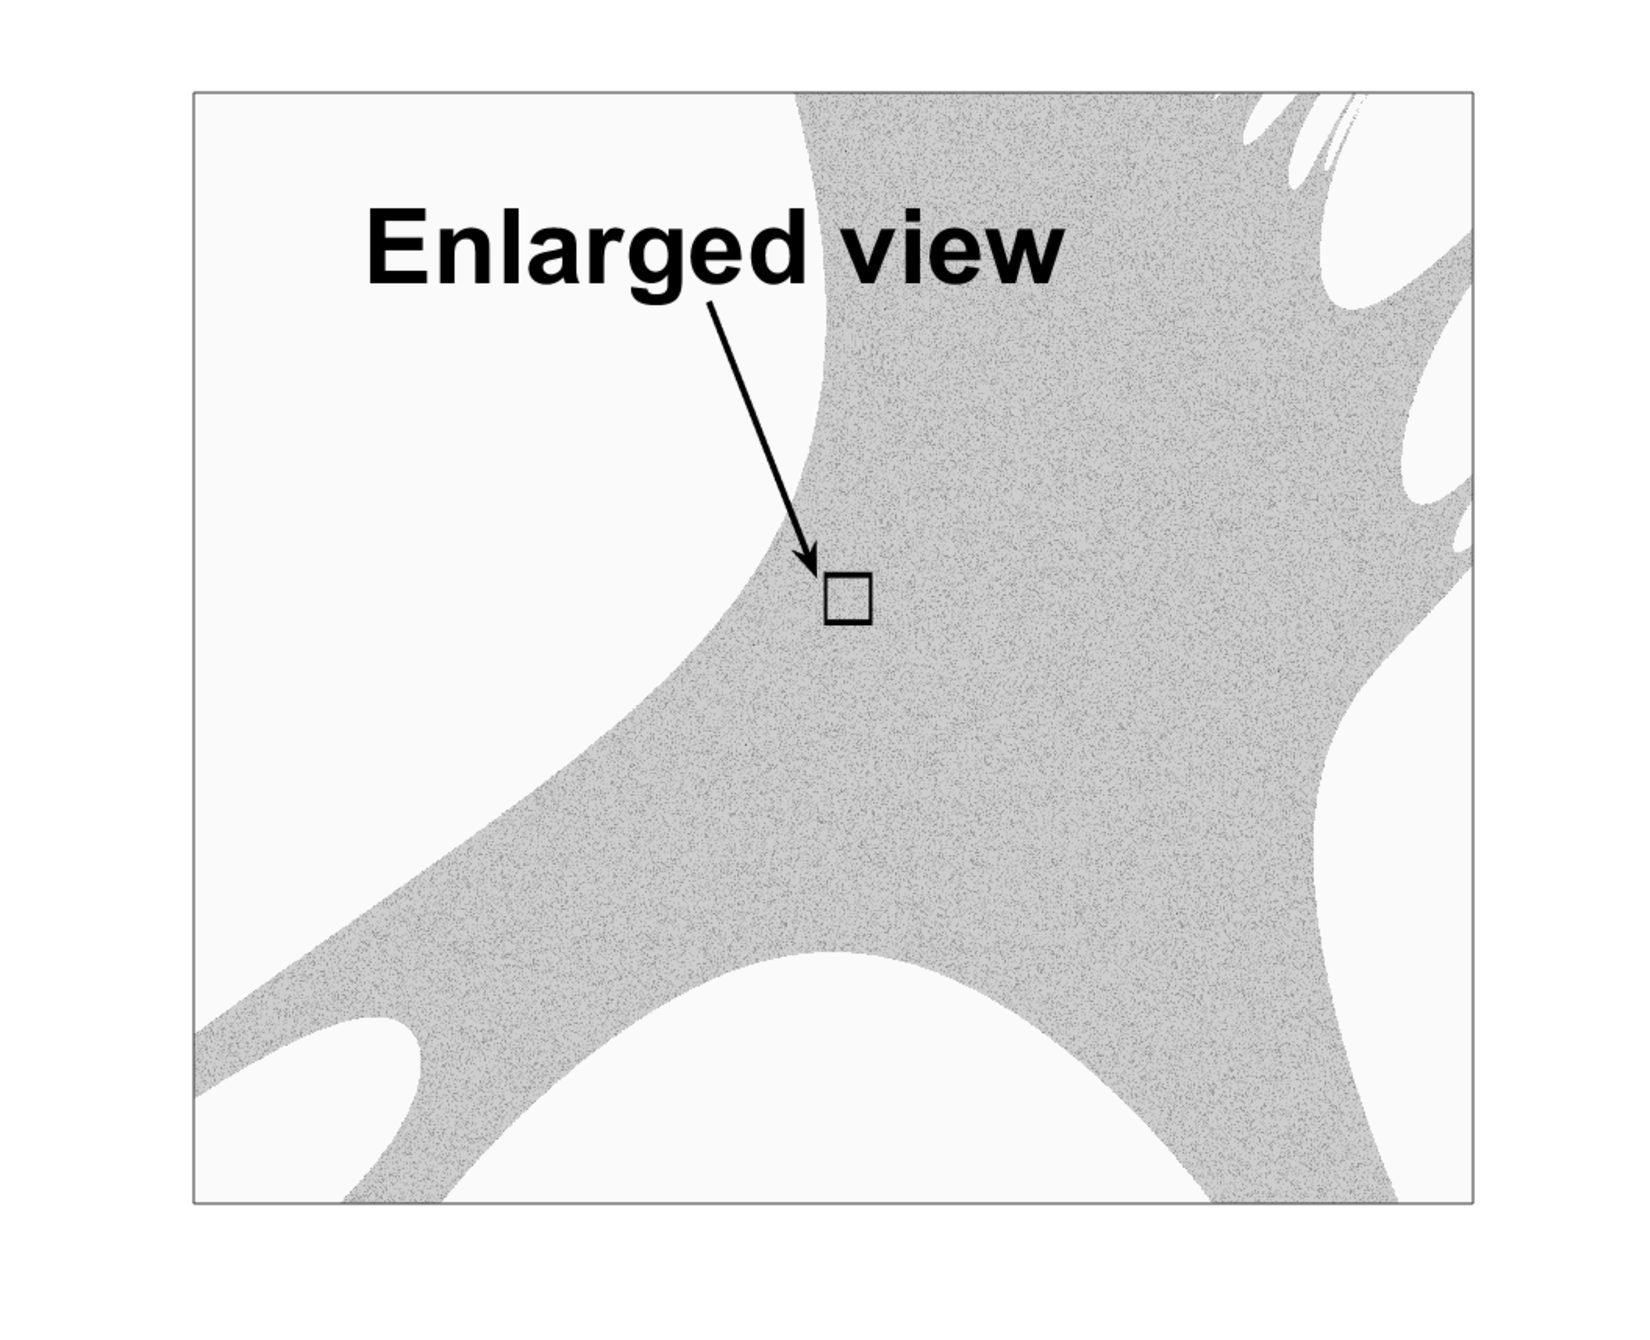
\includegraphics[width=\textwidth]{m_zoom}
        \caption{Rectangular section of the attraction domain, section $[0.3\pm 0.001, -0.2\pm 0.001]$.}
        \label{fig:gull}
    \end{subfigure}
    \hfill 
    \begin{subfigure}[t]{0.49\textwidth}
        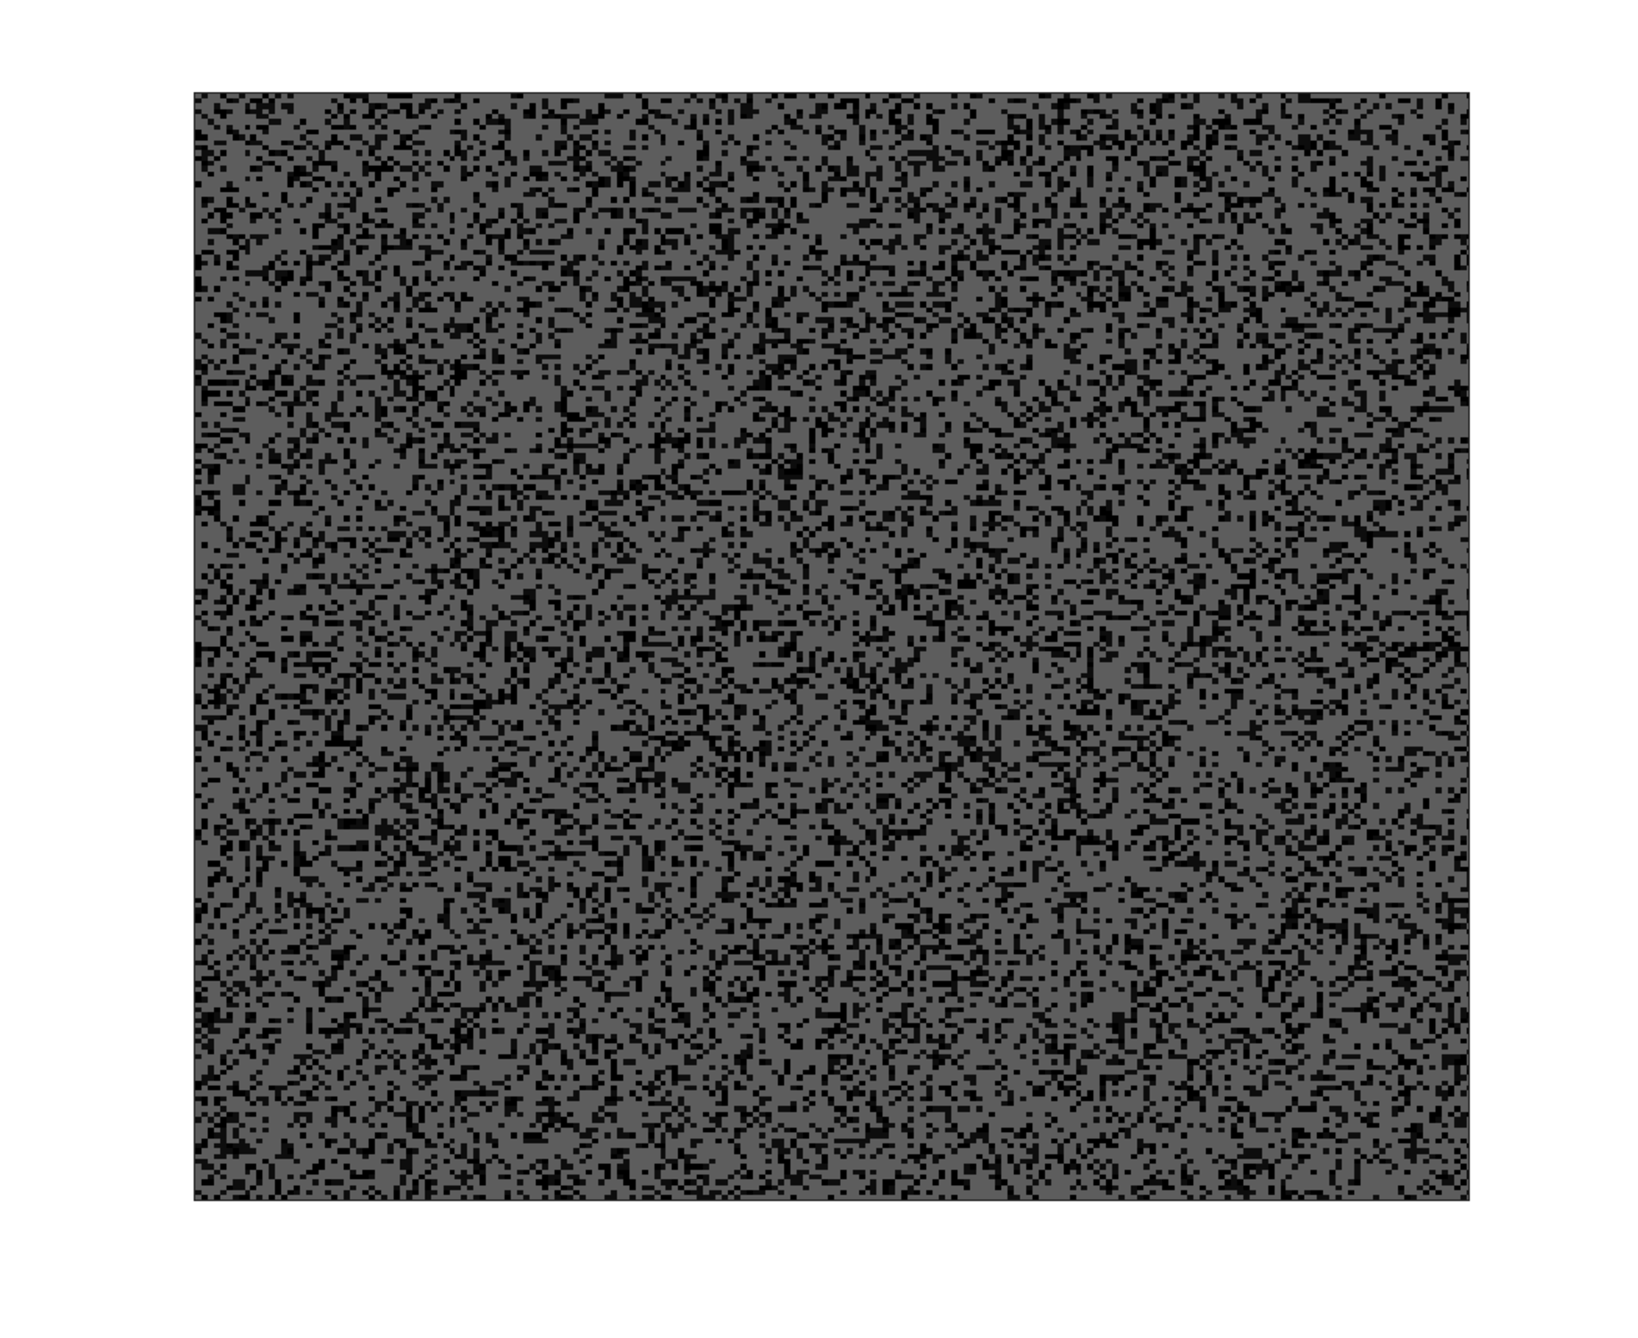
\includegraphics[width=\textwidth]{m14_lu_zoomO}
        \caption{$n_f=14$.}
        \label{fig:tiger}
    \end{subfigure}
   \hfill  
    \begin{subfigure}[t]{0.49\textwidth}
        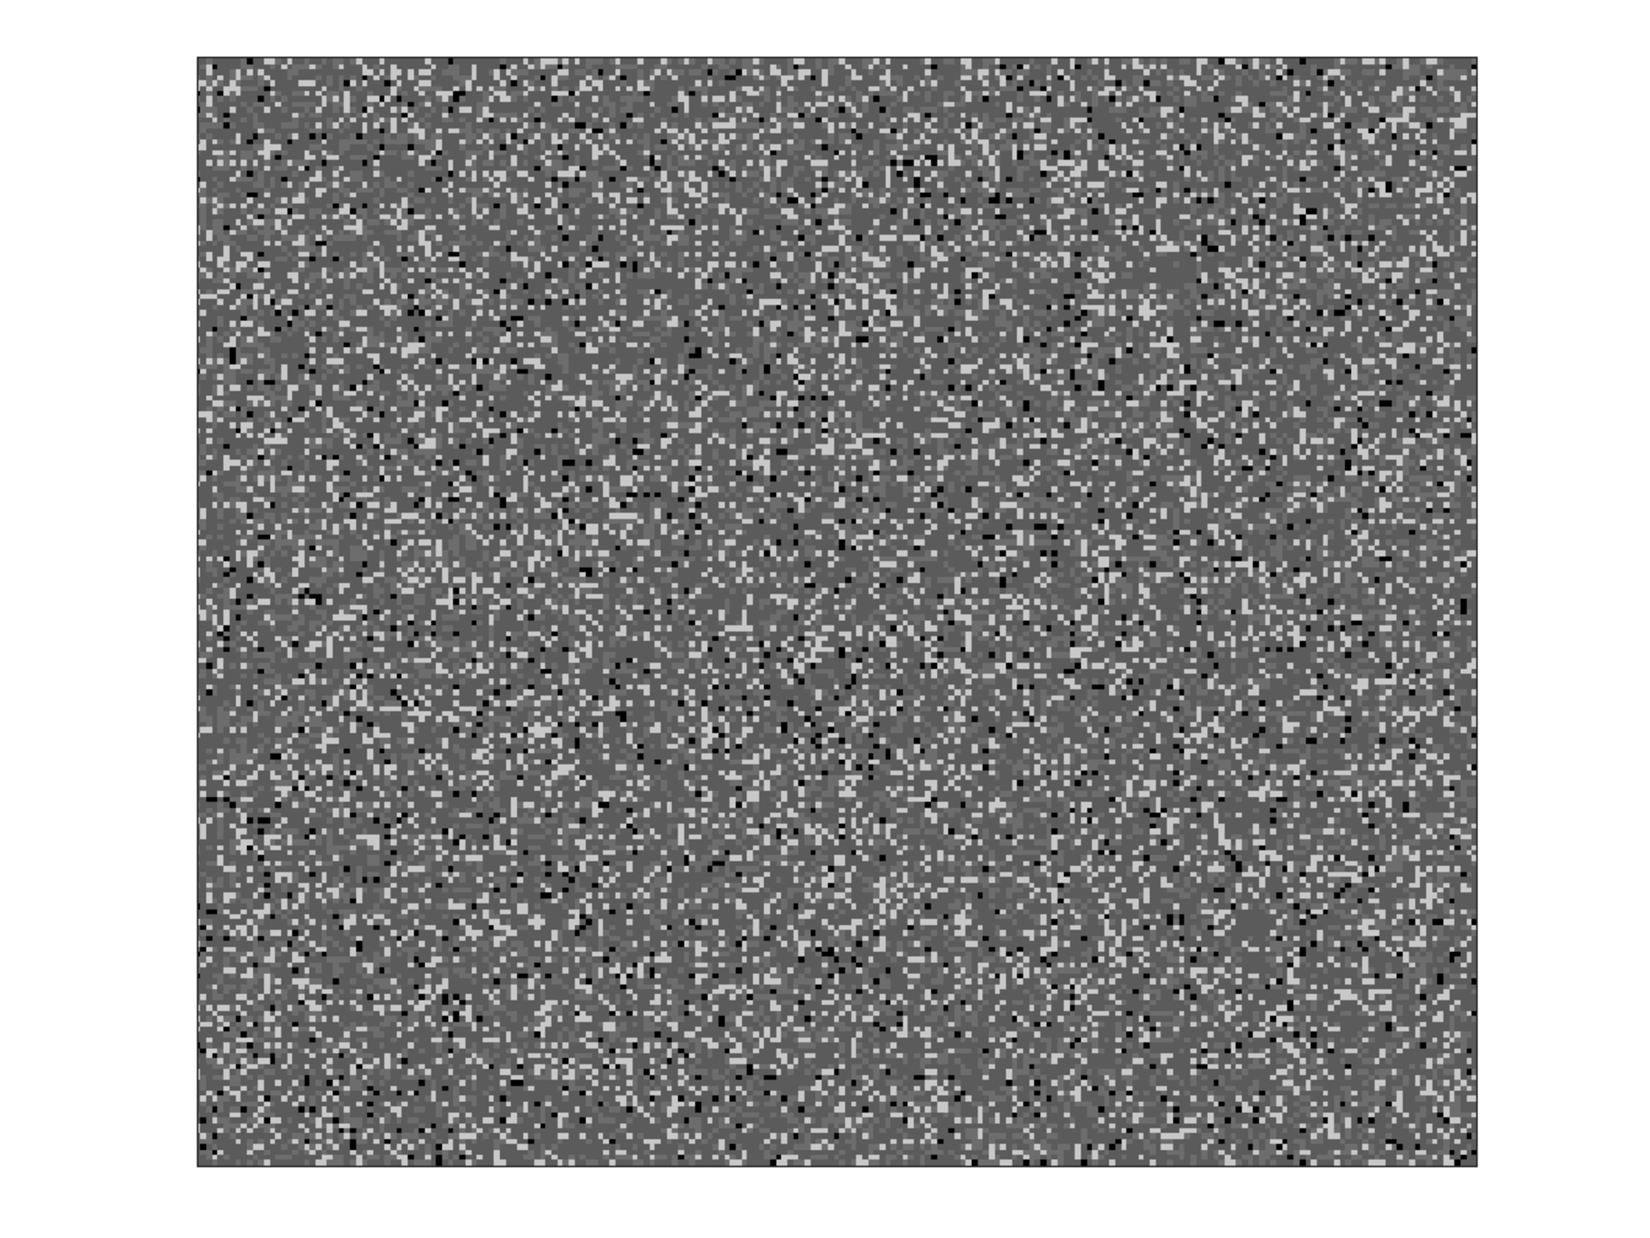
\includegraphics[width=\textwidth]{m17_lu_zoomO}
        \caption{$n_f=17$.}
        \label{fig:mouse}
    \end{subfigure}
  \hfill   
    \begin{subfigure}[t]{0.49\textwidth}
        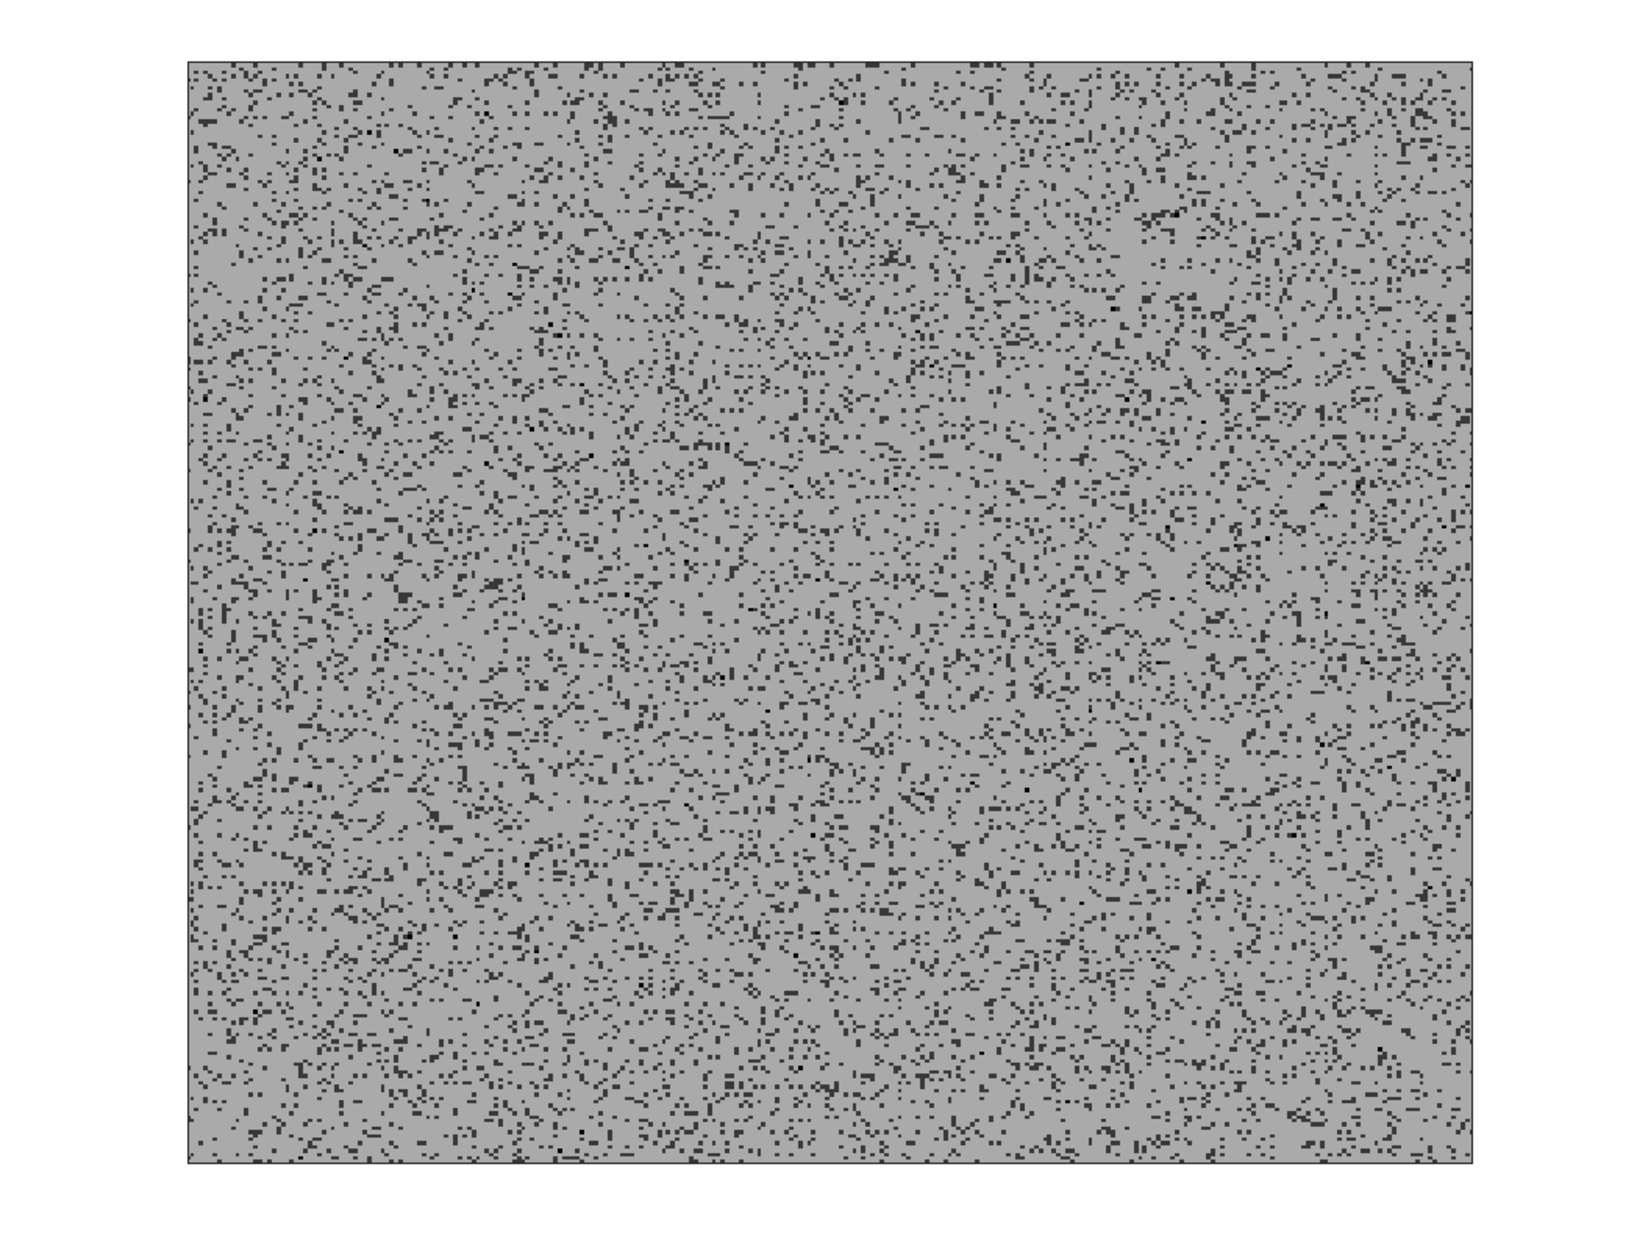
\includegraphics[width=\textwidth]{m18_lu_zoomO}
        \caption{$n_f=18$.}
        \label{fig:mouse}
    \end{subfigure}
    \caption{Enlarged views of sections of the attraction domains for higher values of $n_f$.}\label{fig:m_zoom}
\end{figure}

Nevertheless, when we want to make a general comparison of what happens to the periods when the precisions are varied a color scale is required, see Fig. \ref{fig:m}.
%
\begin{figure*}
\centering
\begin{tabular}{cc}
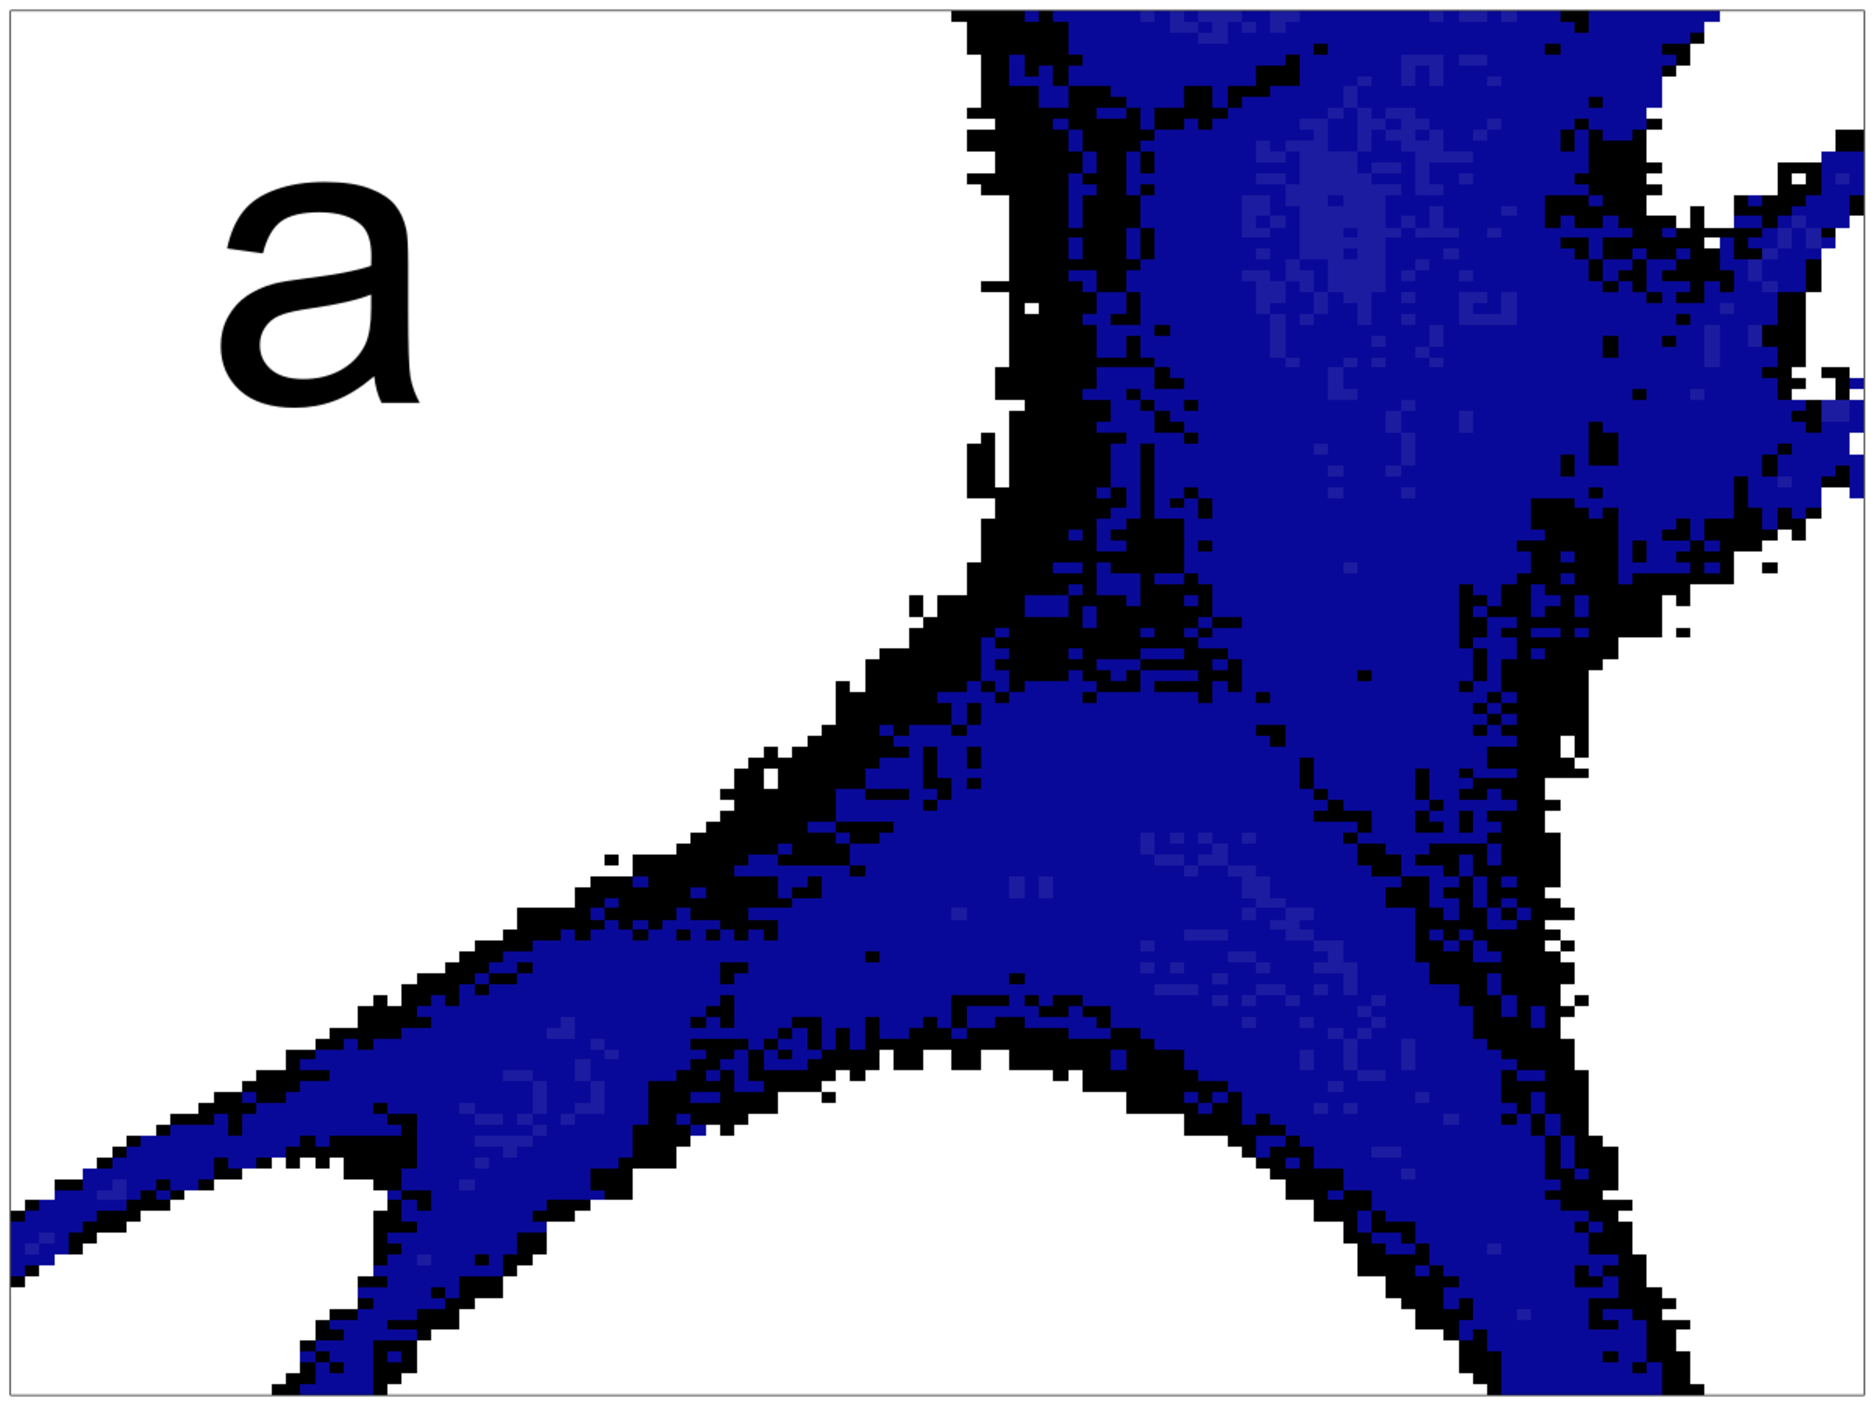
\includegraphics[width=0.35\textwidth]{m5}
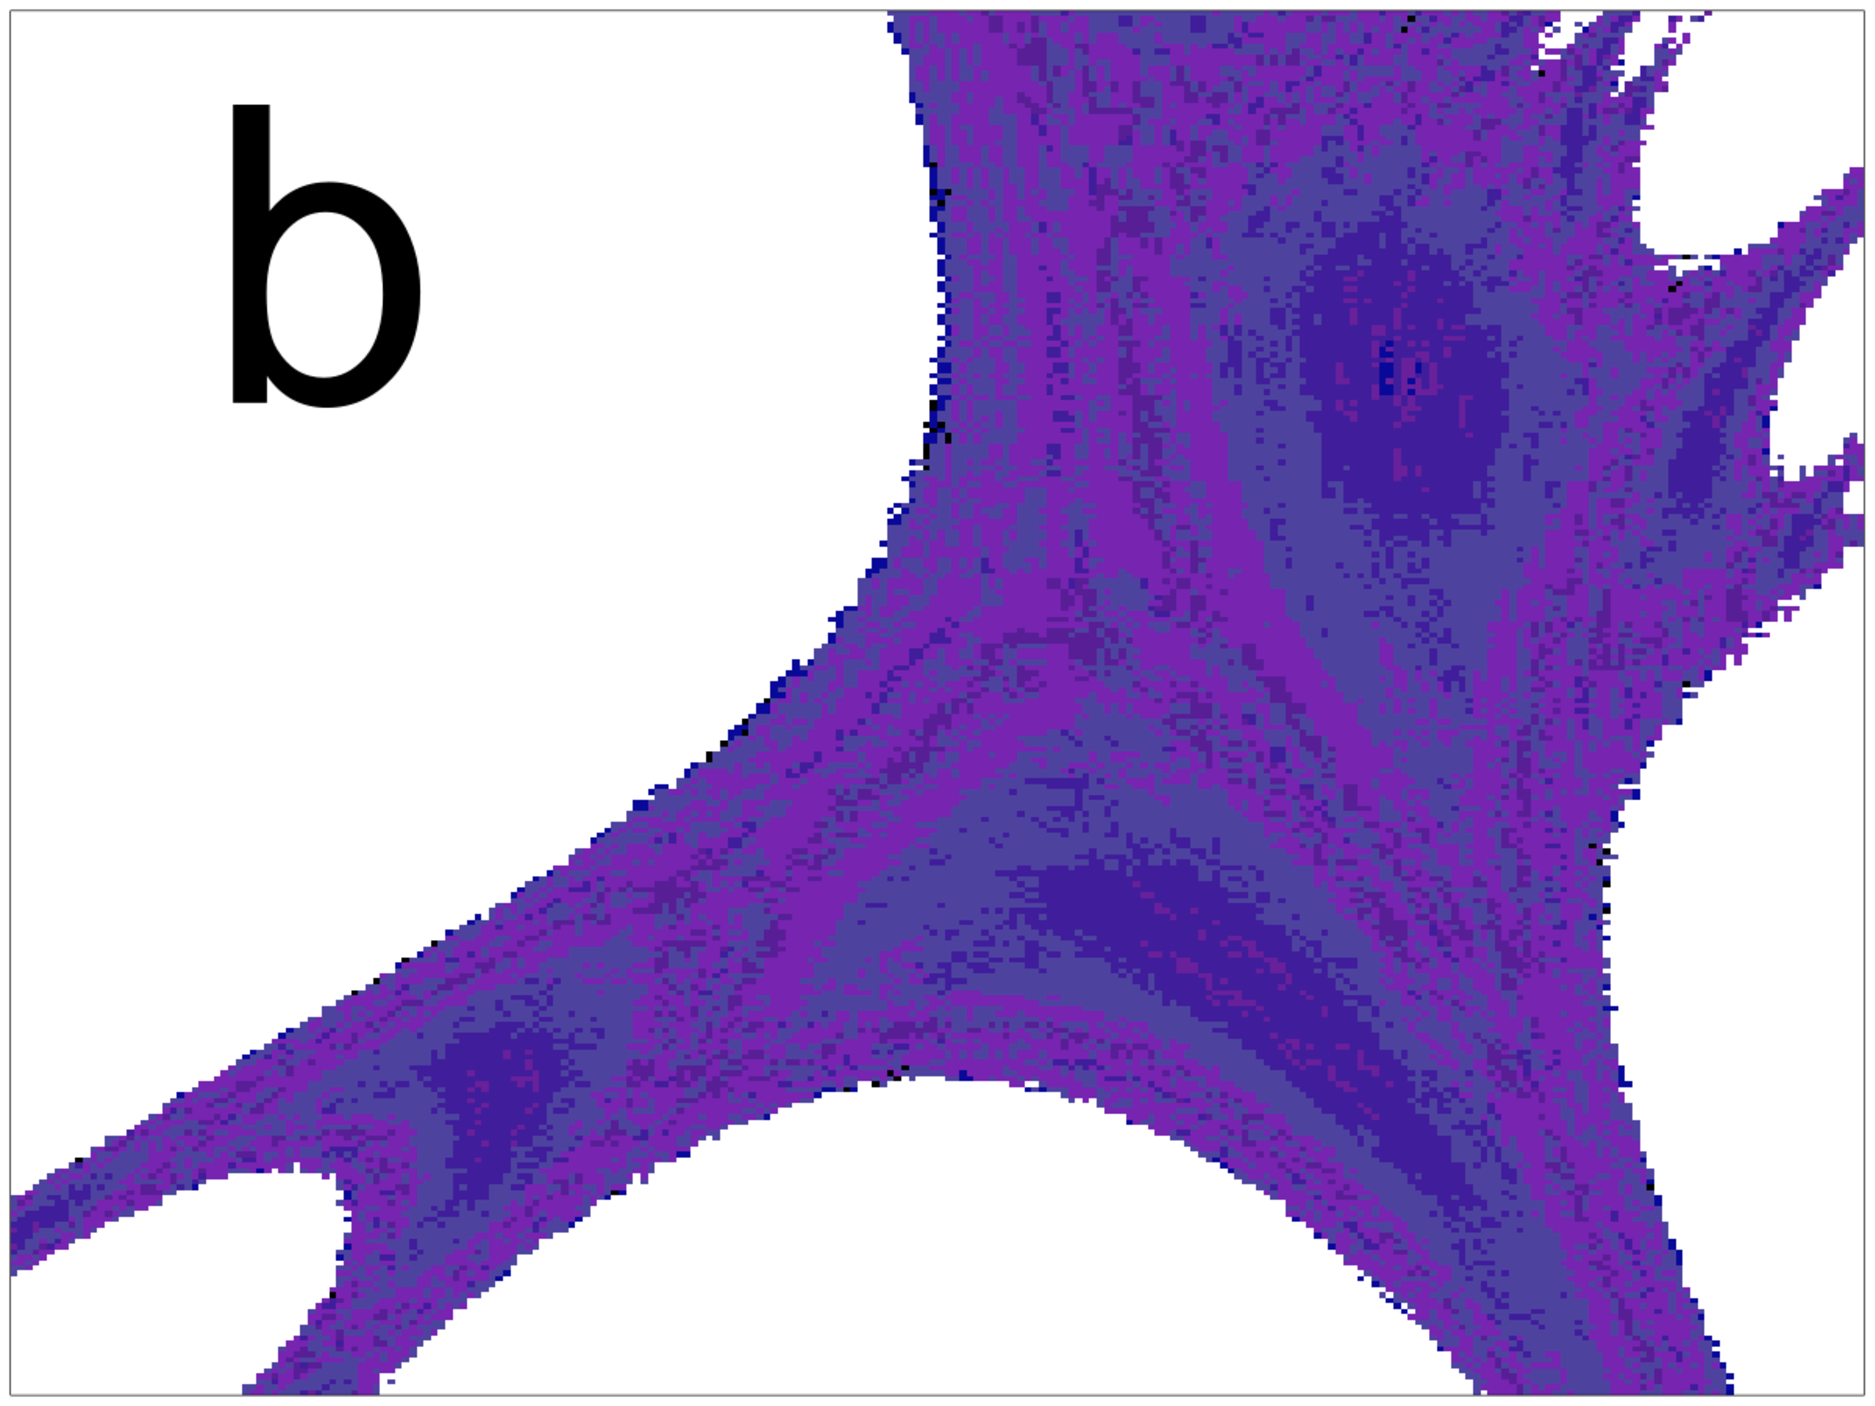
\includegraphics[width=0.35\textwidth]{m6}
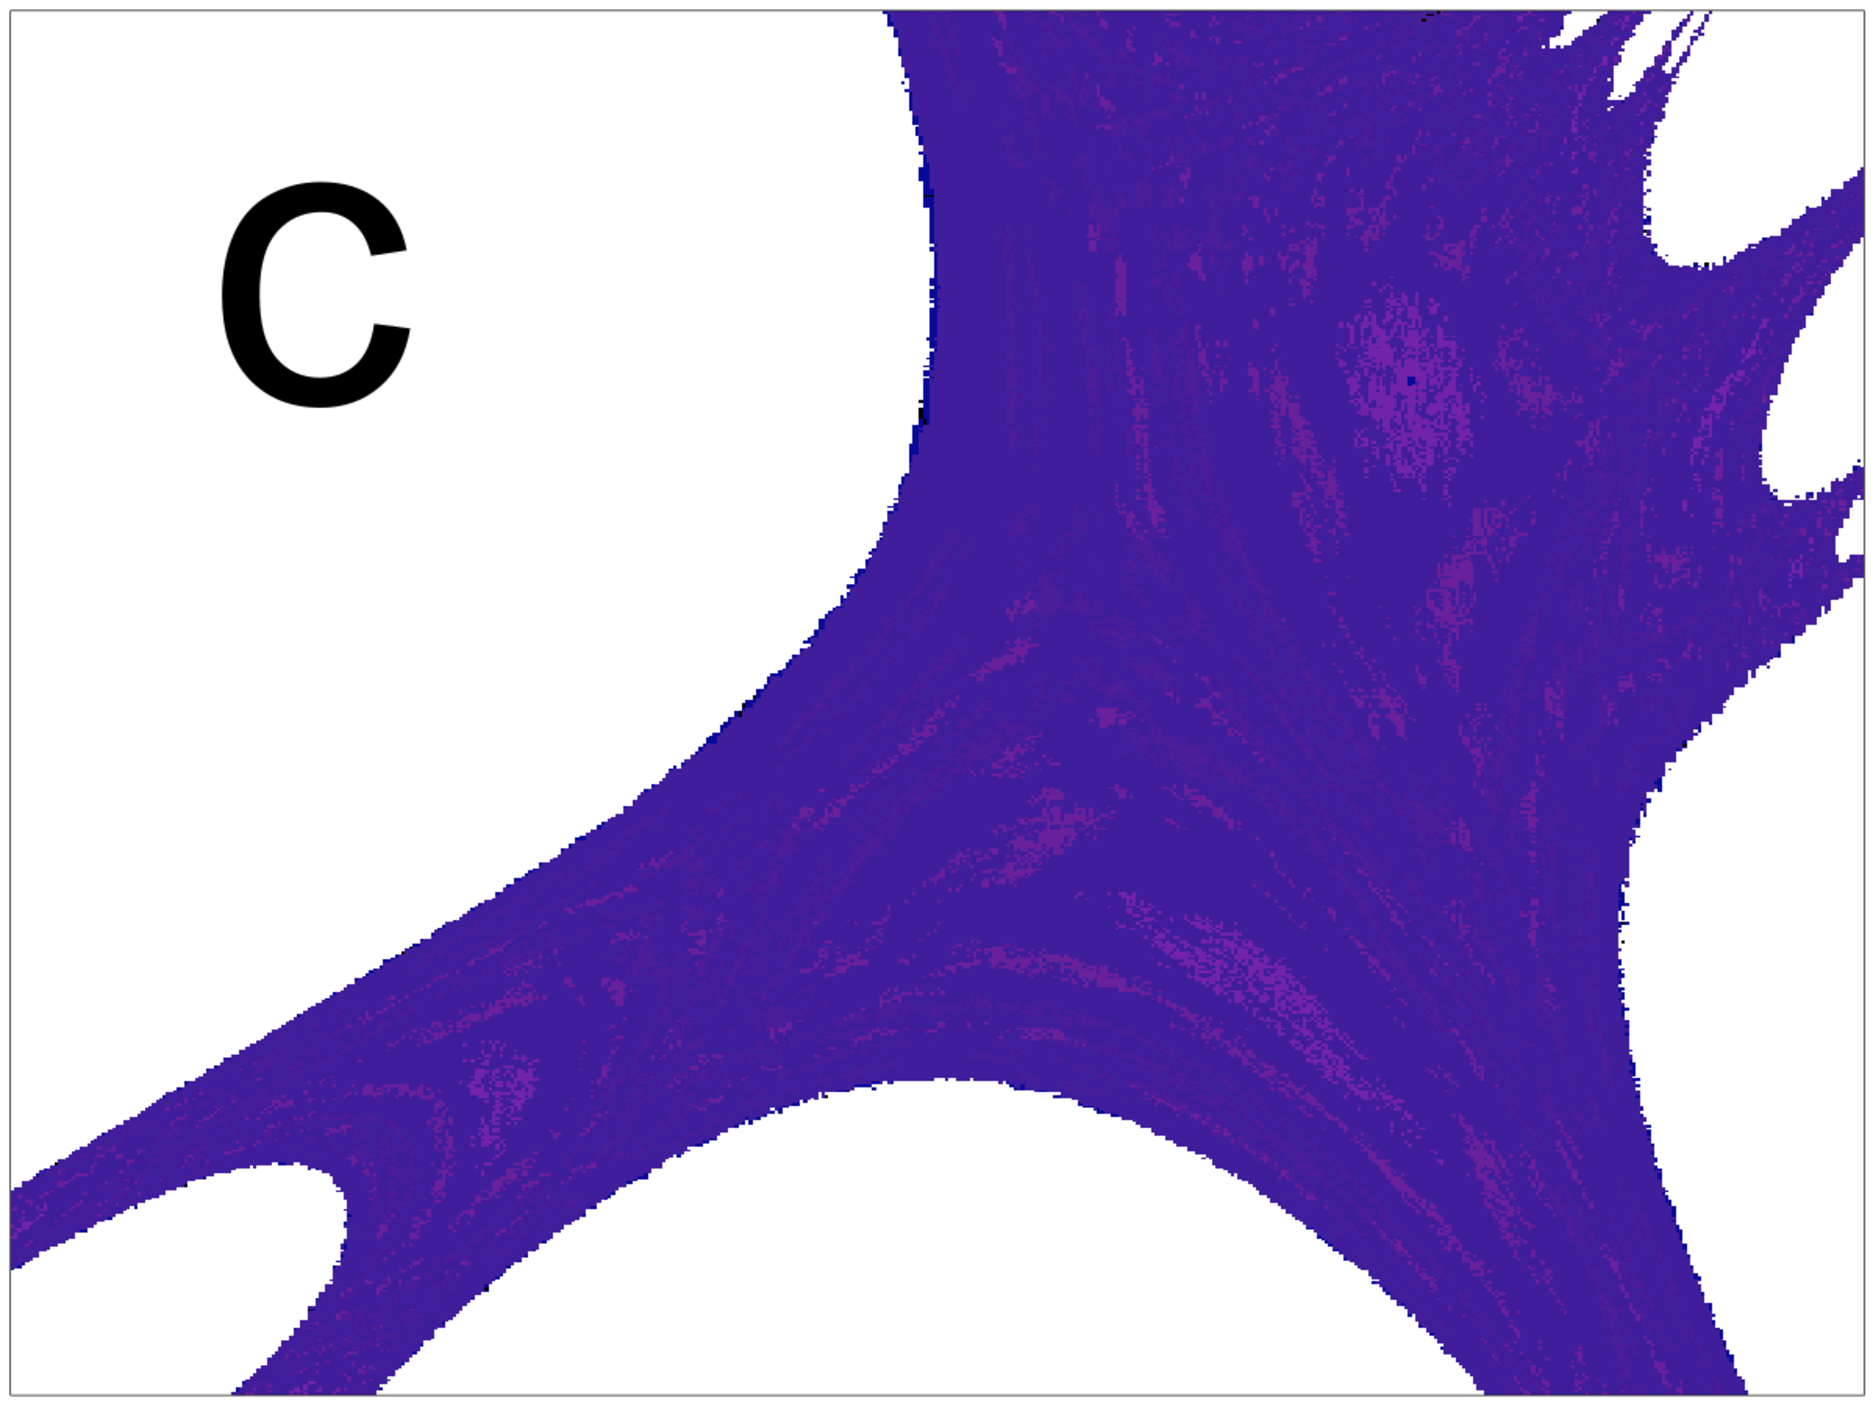
\includegraphics[width=0.35\textwidth]{m7}\\
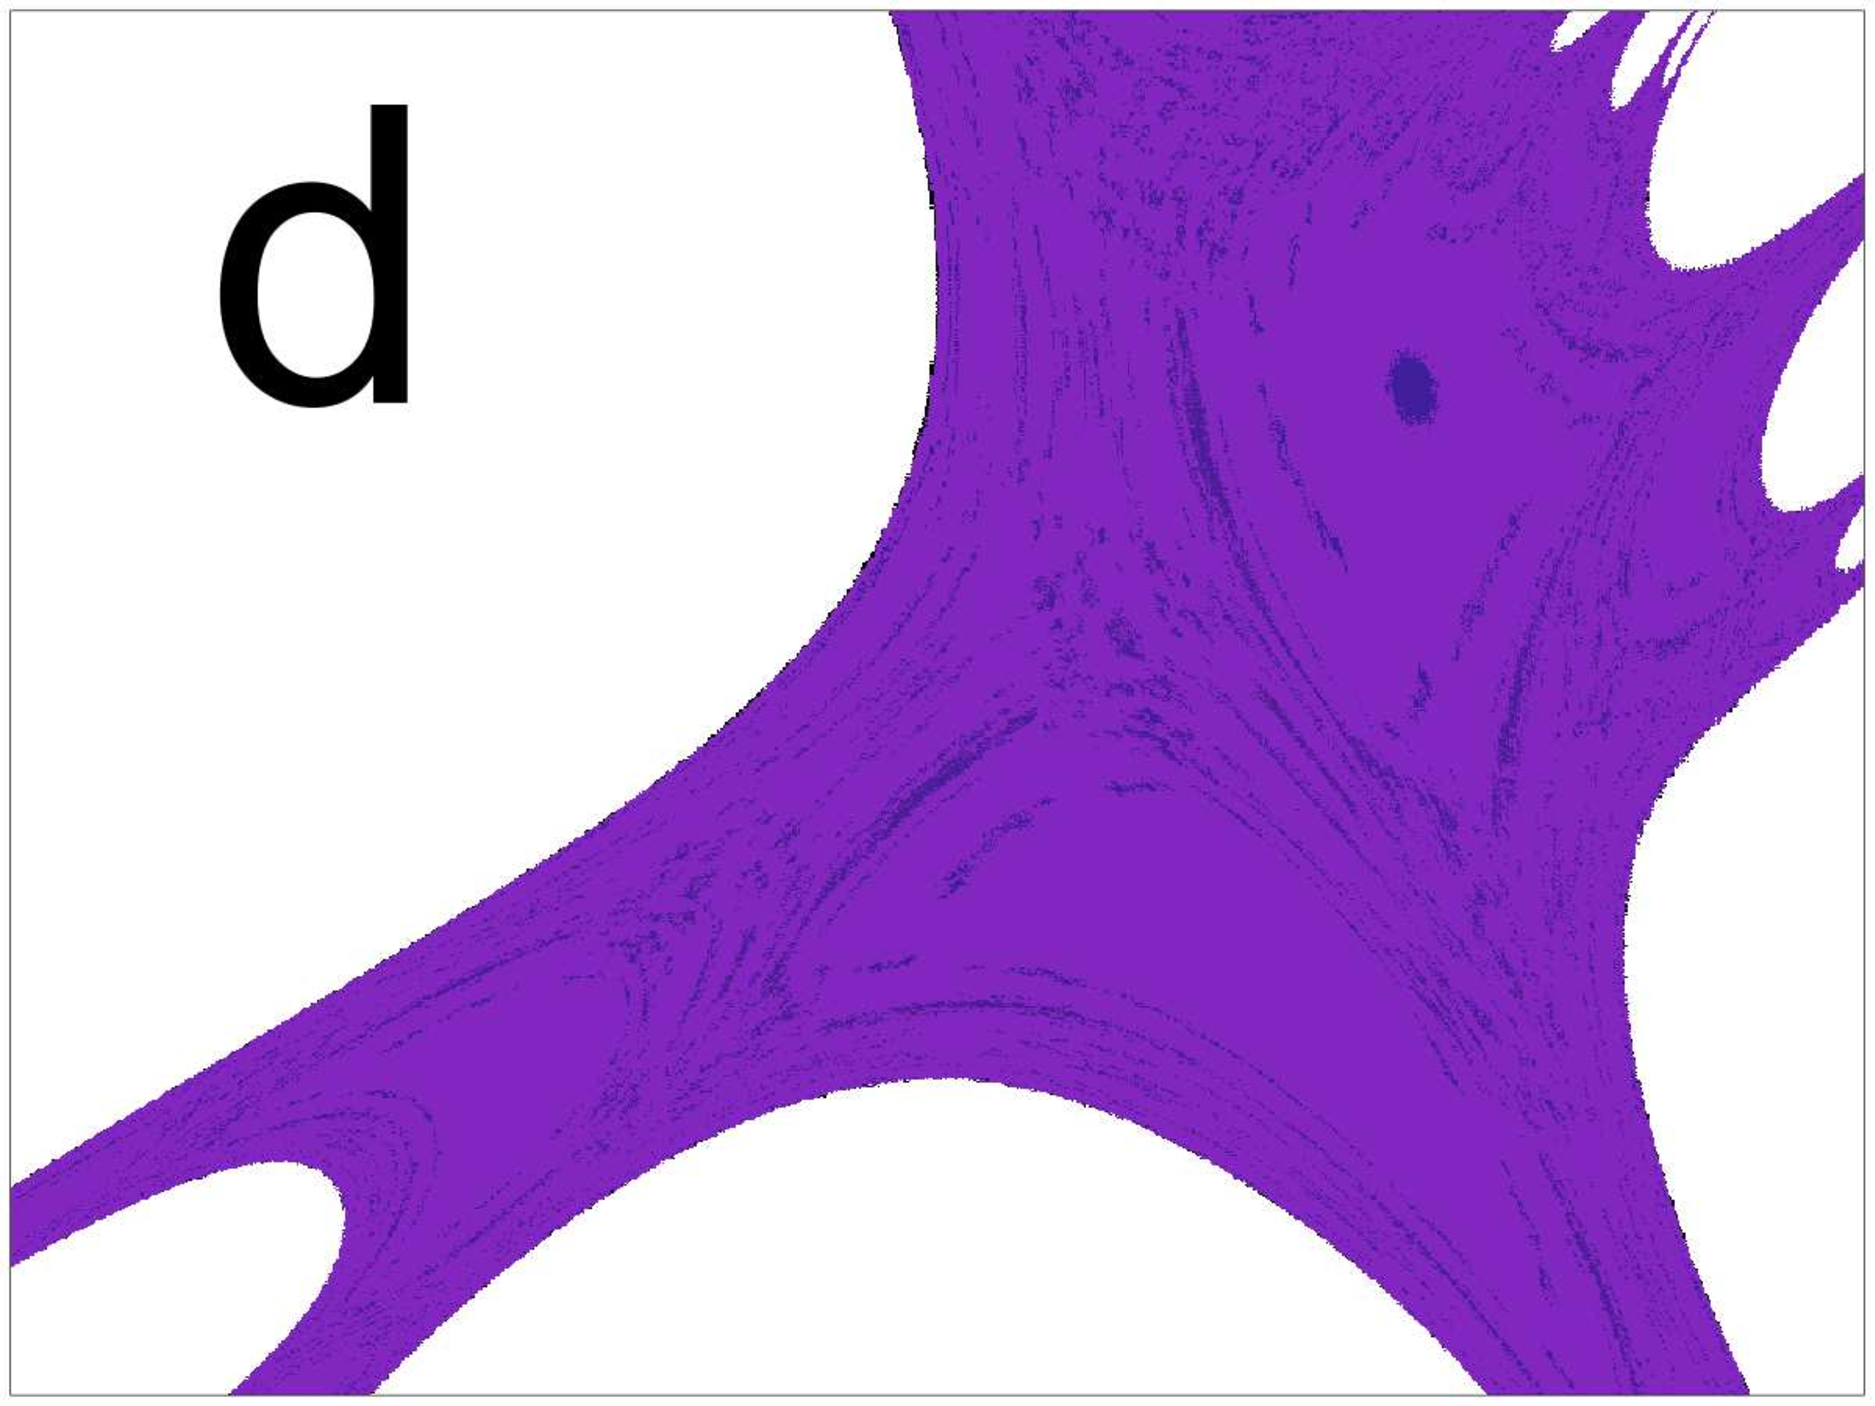
\includegraphics[width=0.35\textwidth]{m8}
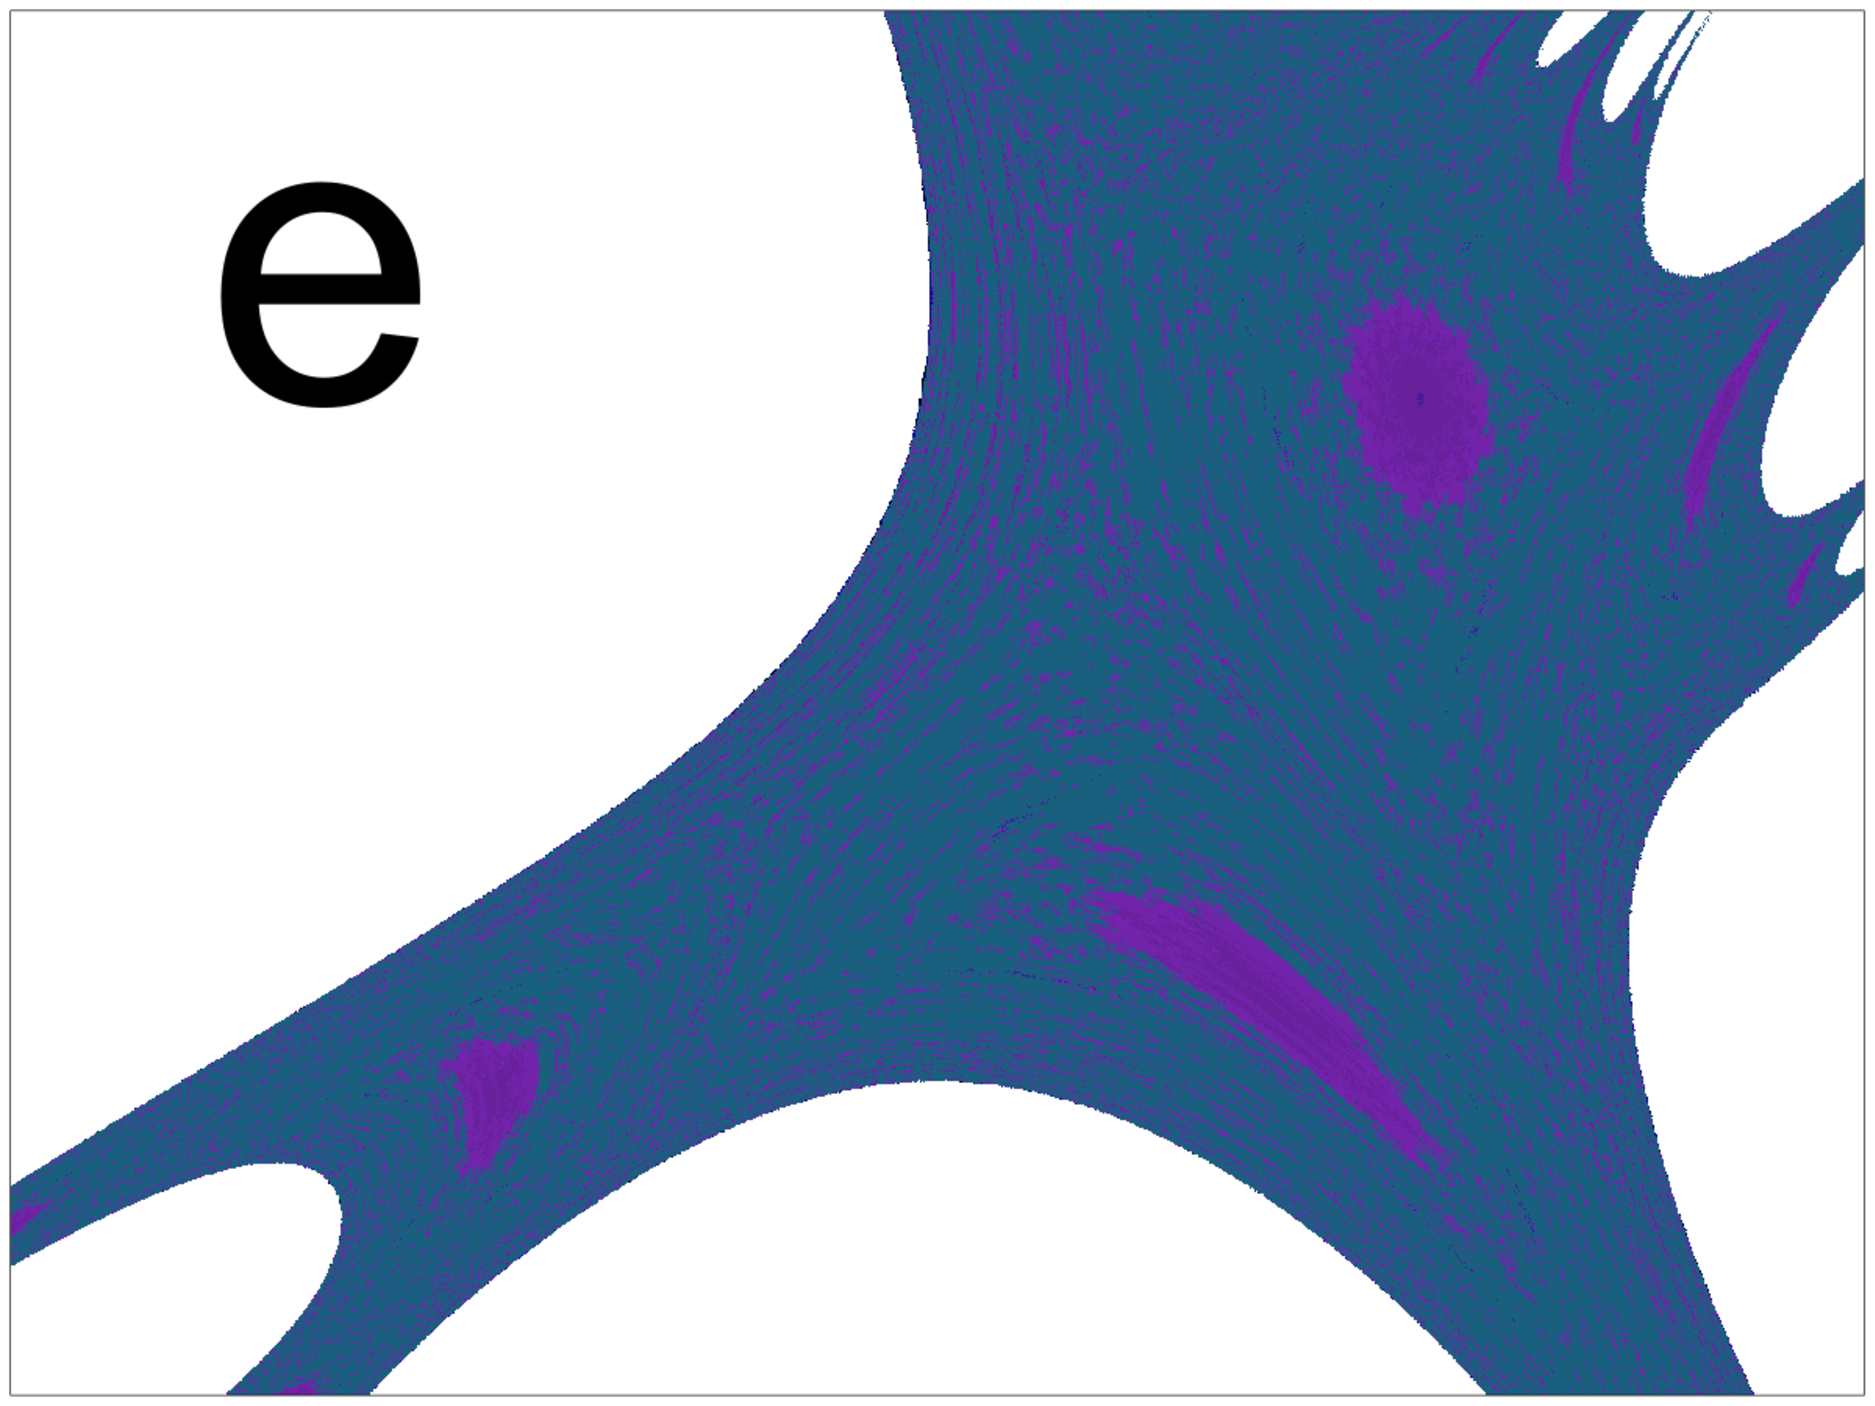
\includegraphics[width=0.35\textwidth]{m9}
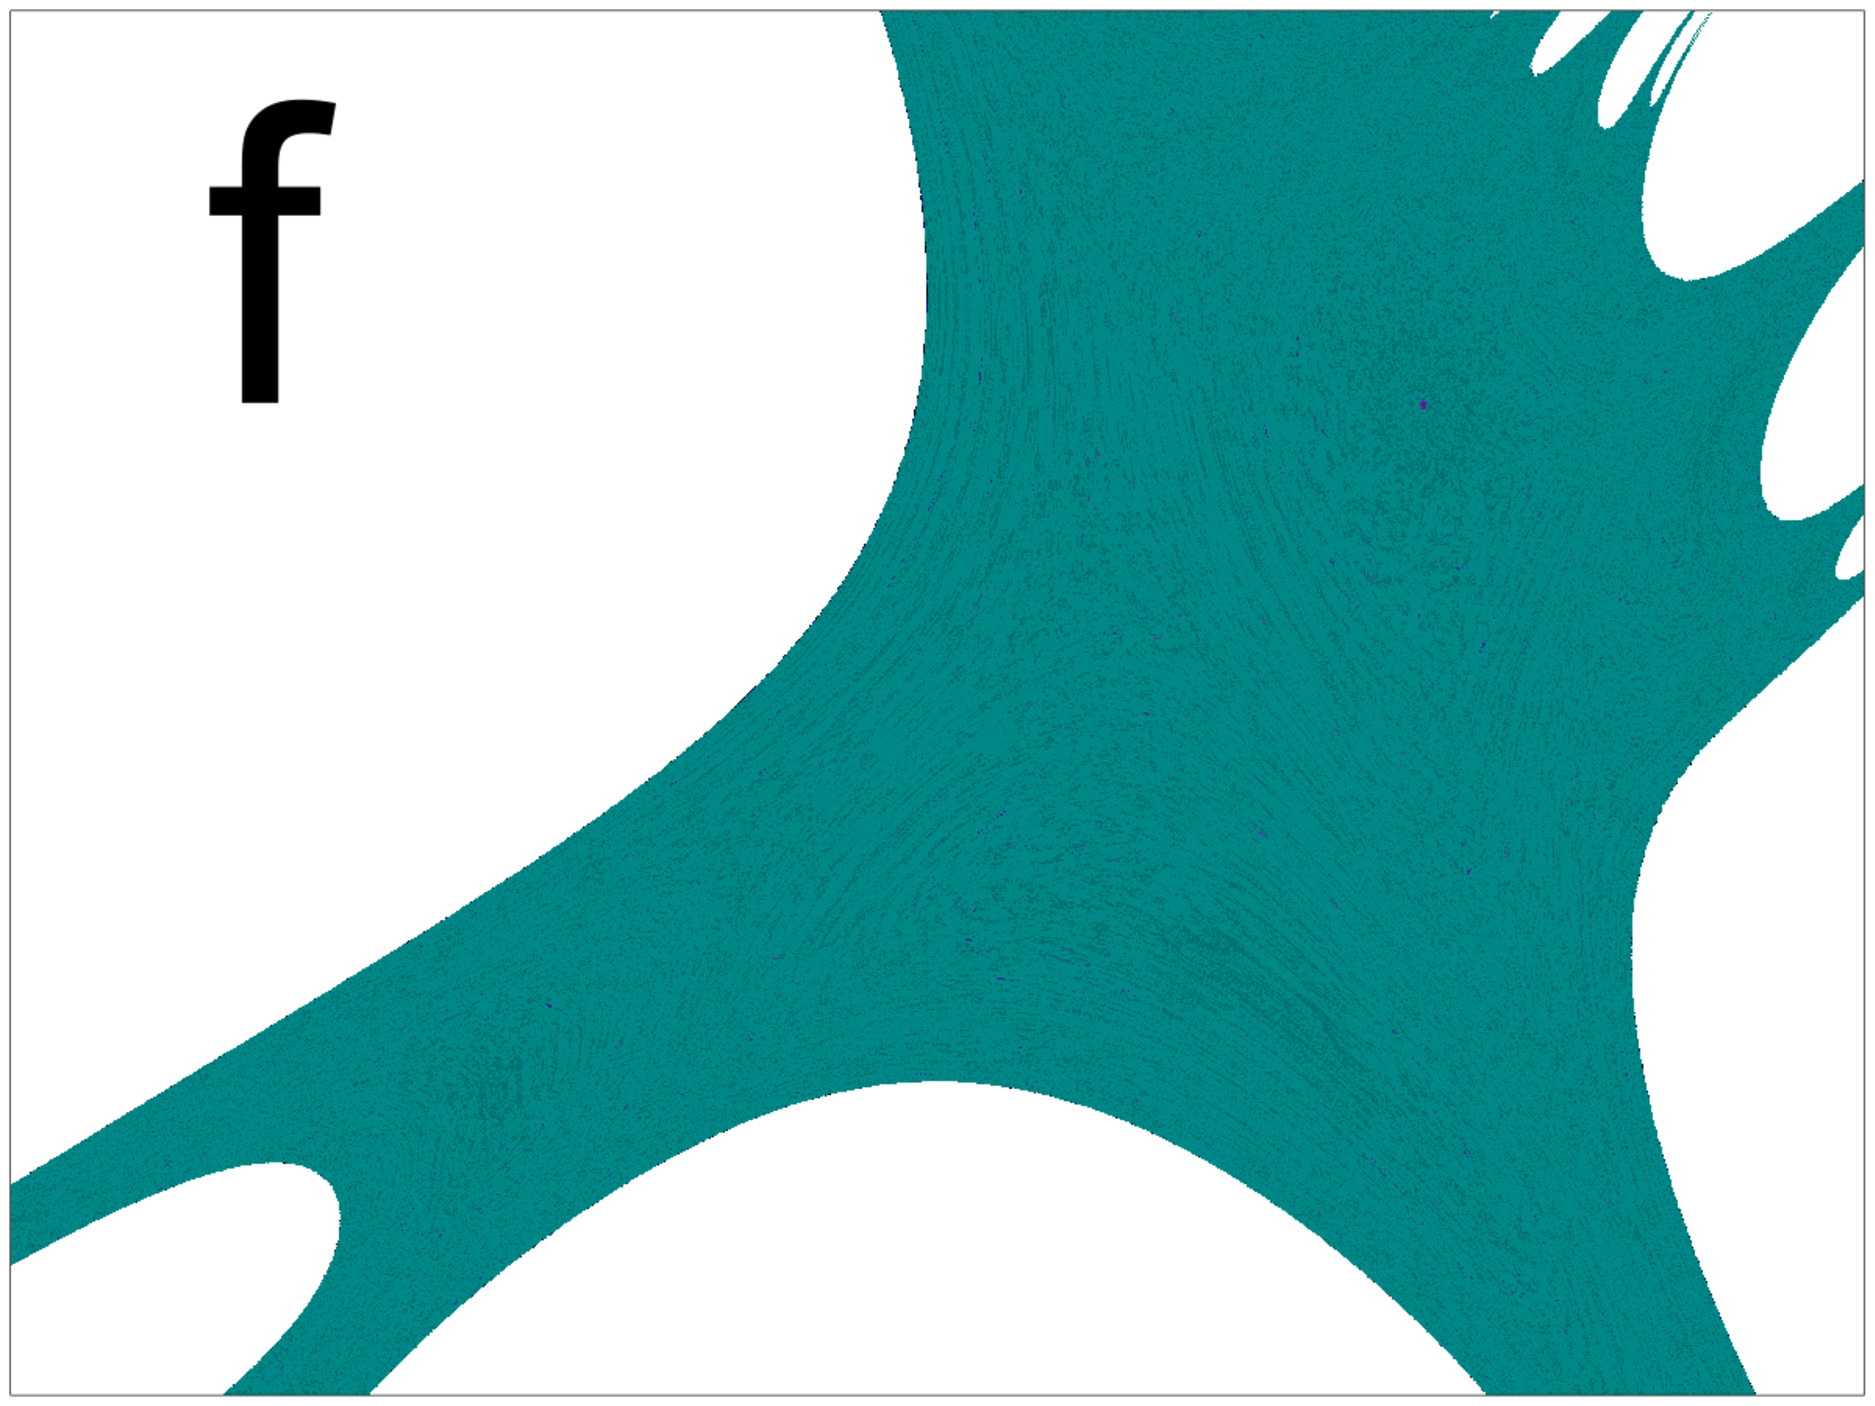
\includegraphics[width=0.35\textwidth]{m10}\\
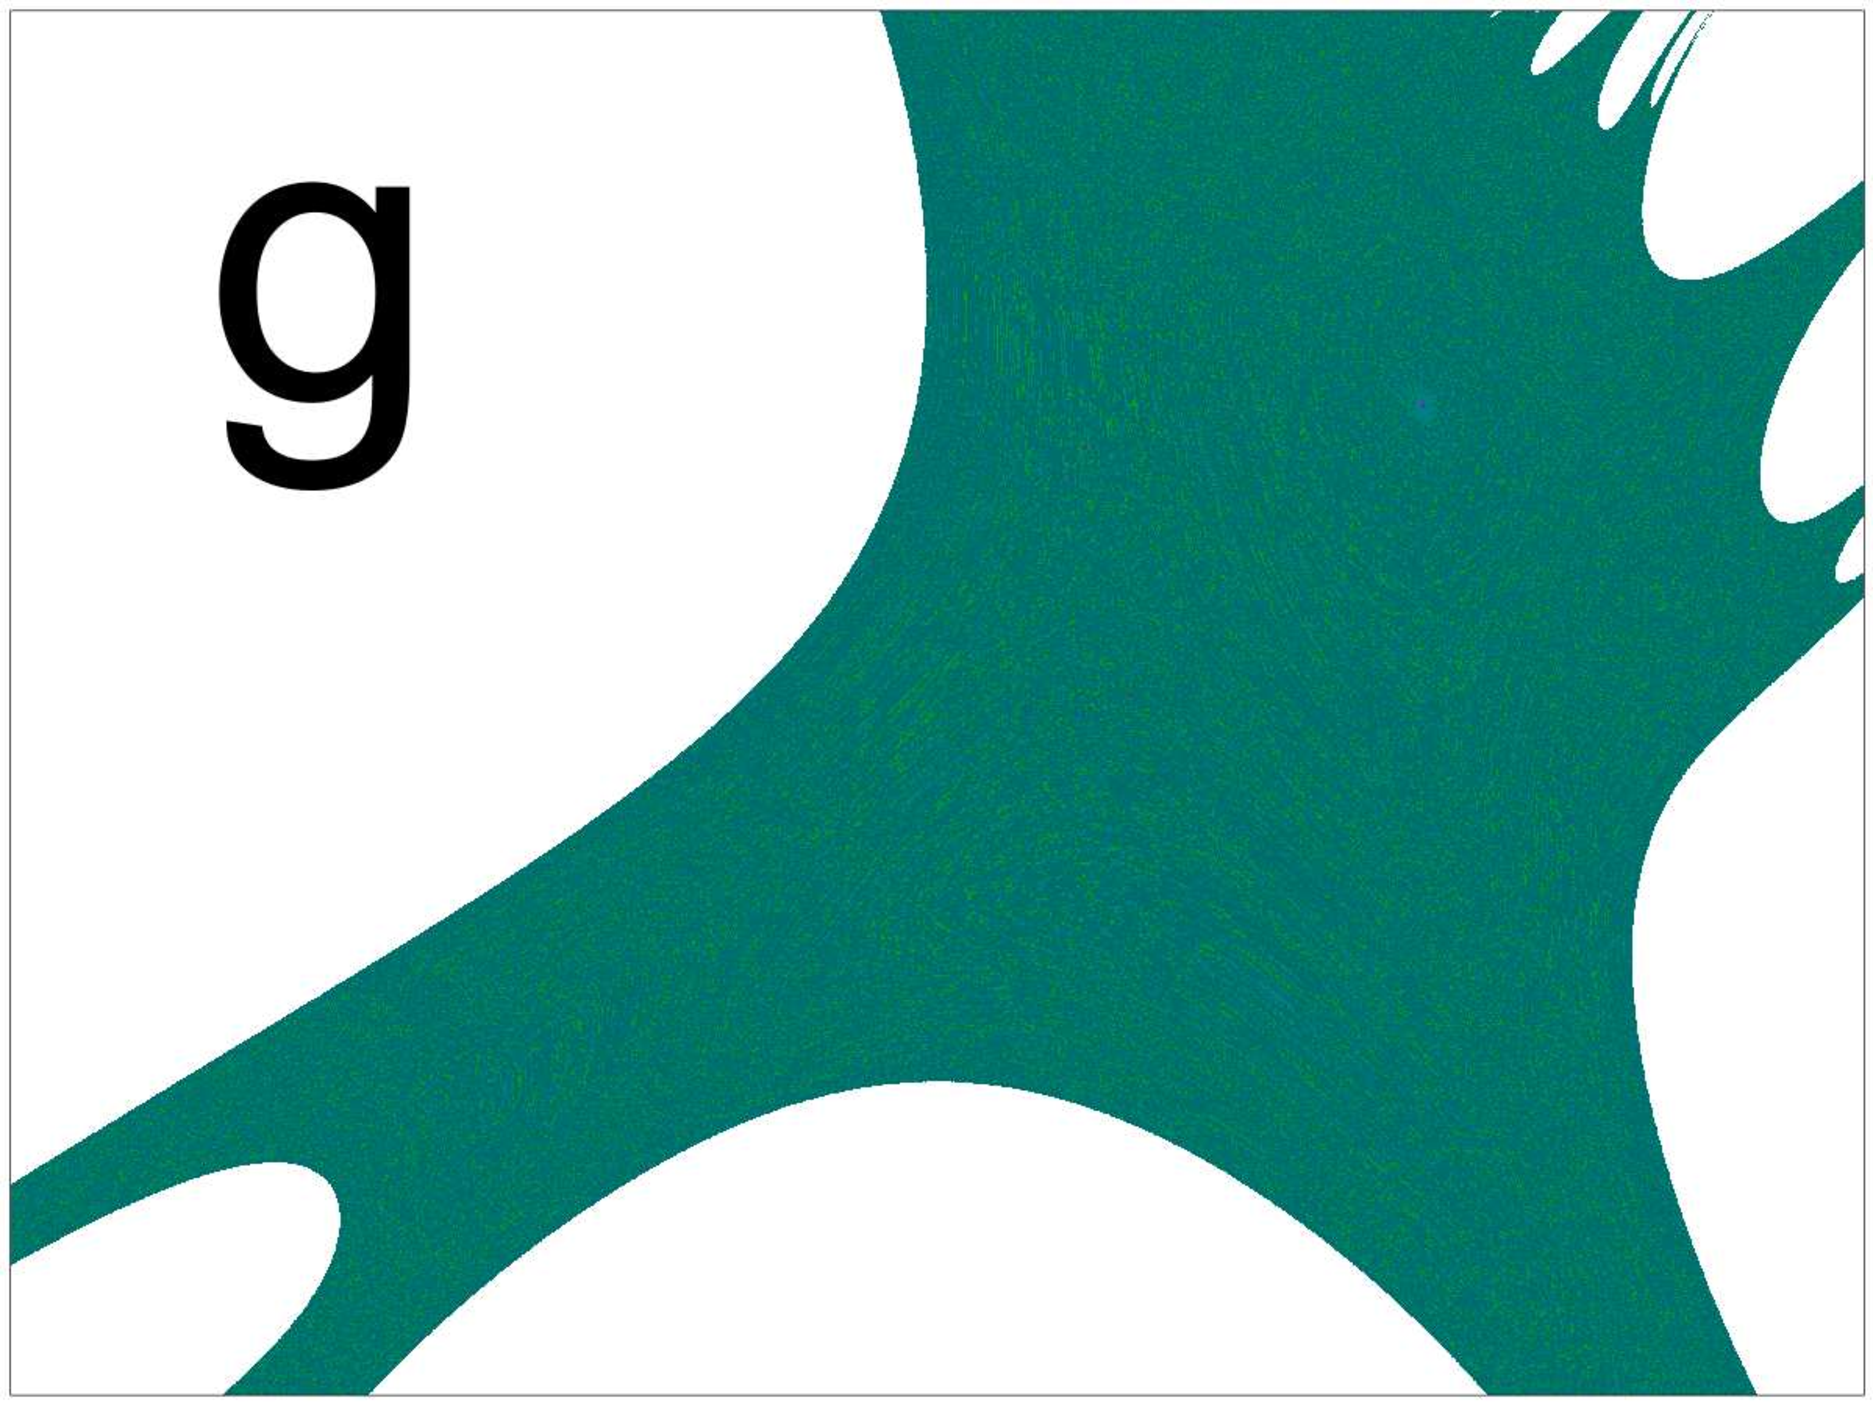
\includegraphics[width=0.35\textwidth]{m11}
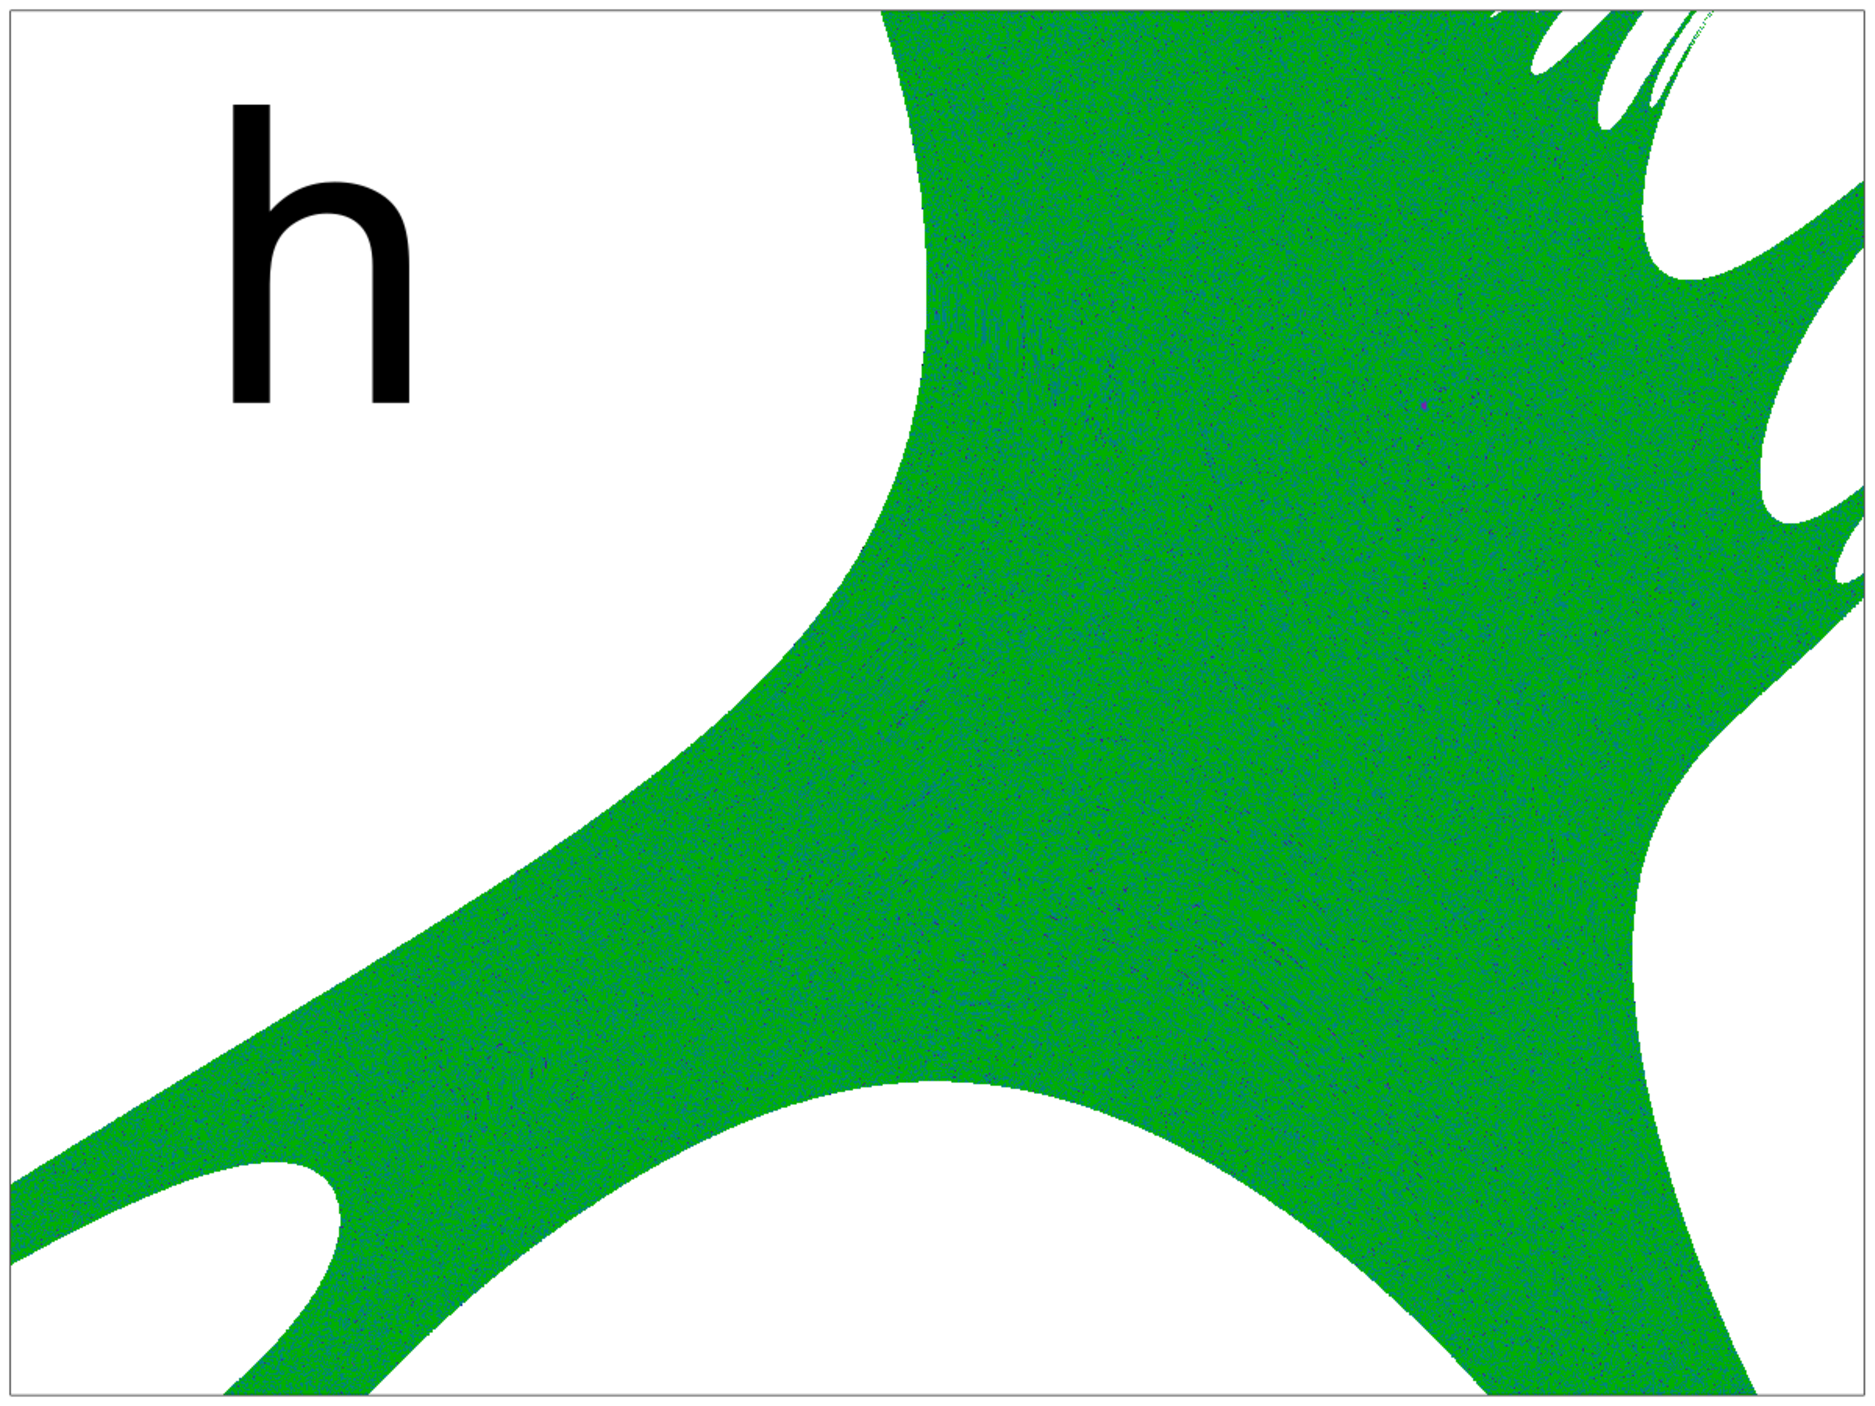
\includegraphics[width=0.35\textwidth]{m12}

\includegraphics[width=0.35\textwidth]{m13}\\

\includegraphics[width=0.35\textwidth]{m14}
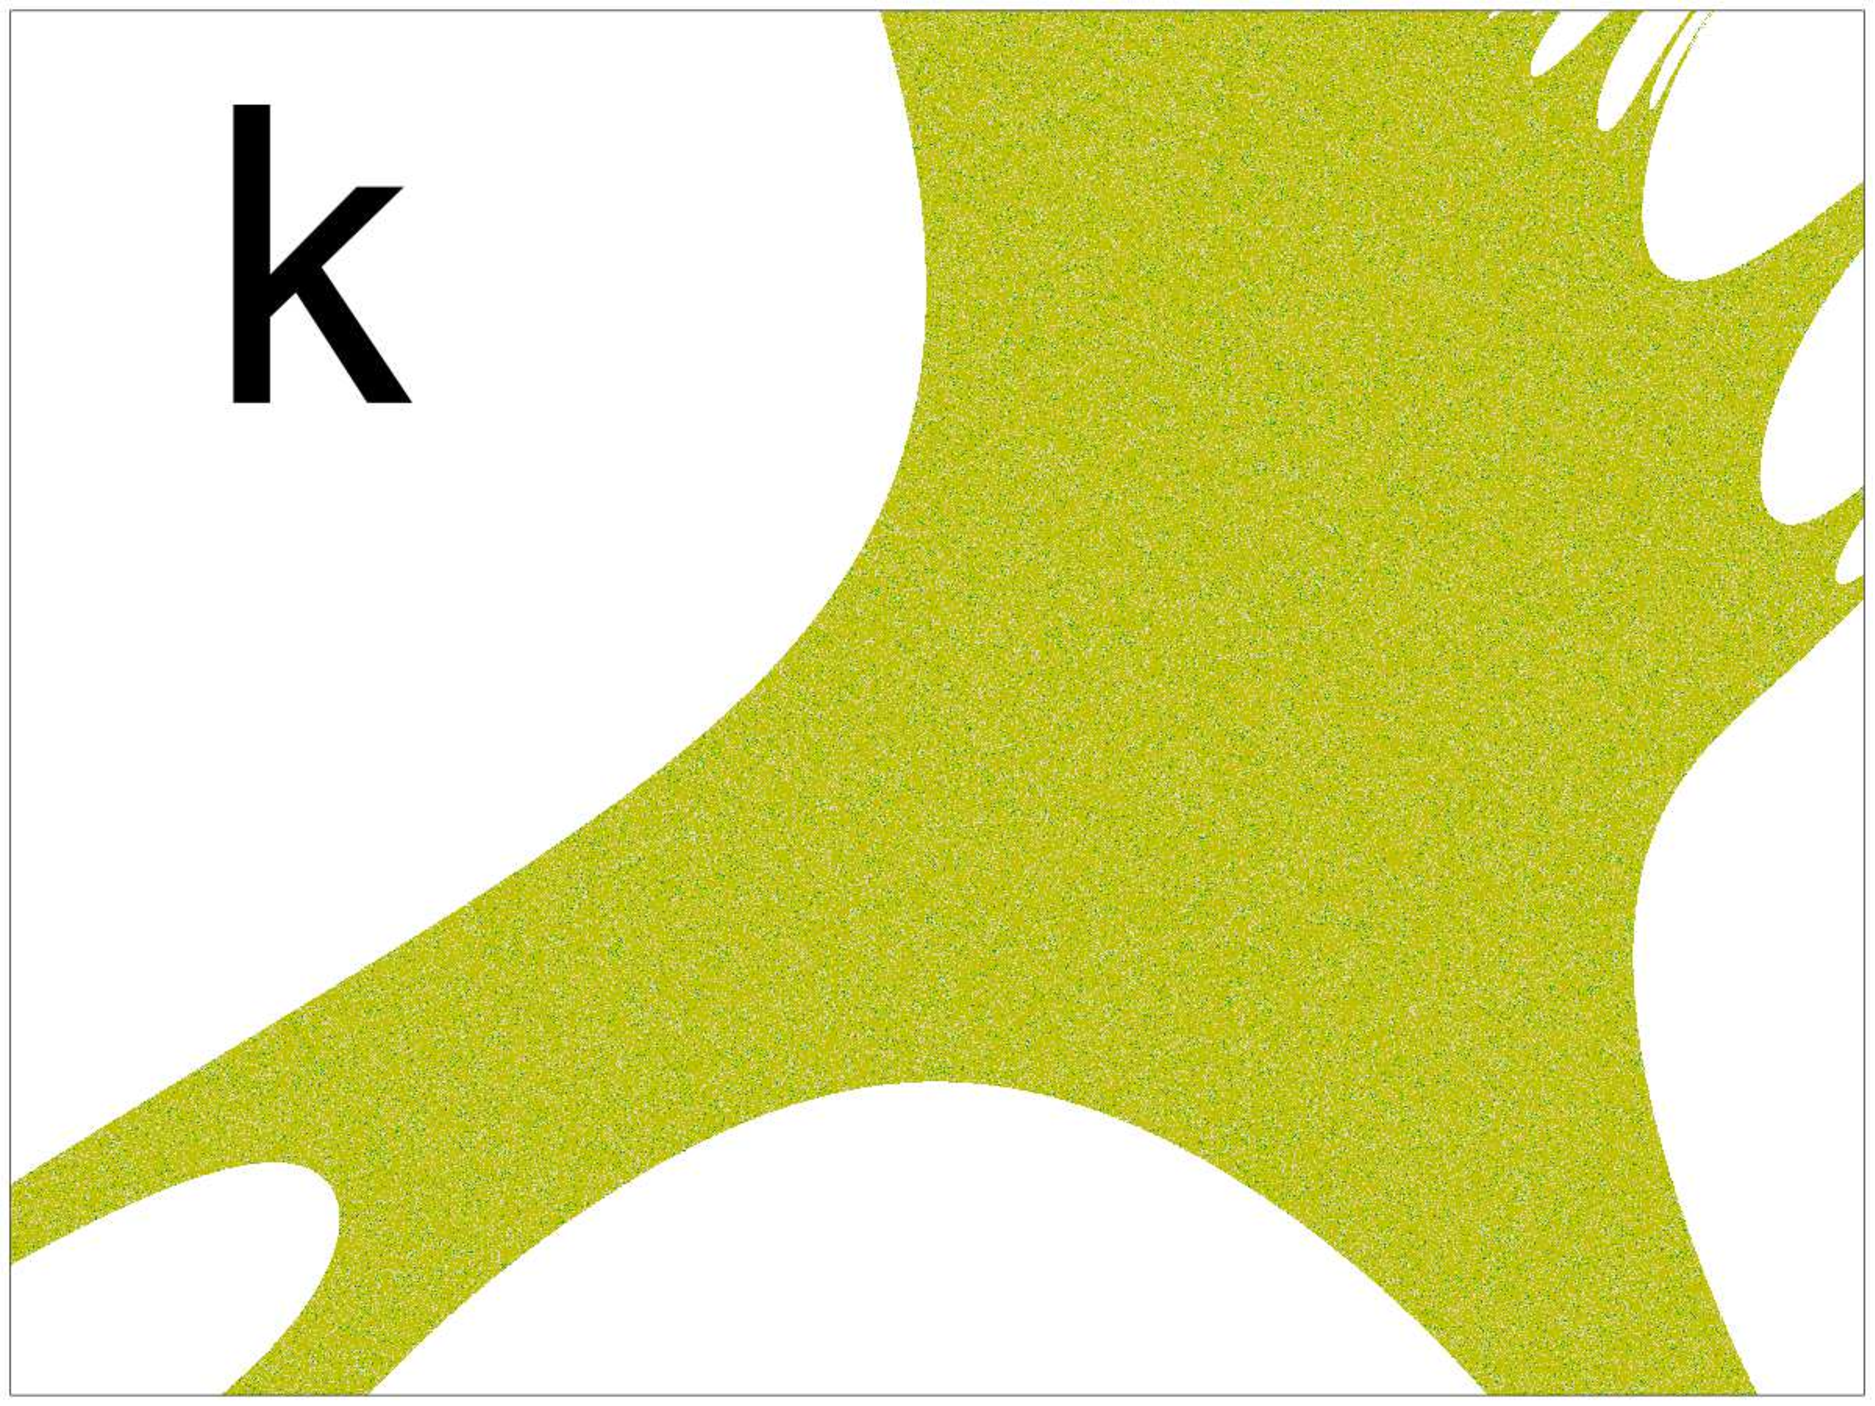
\includegraphics[width=0.35\textwidth]{m17}
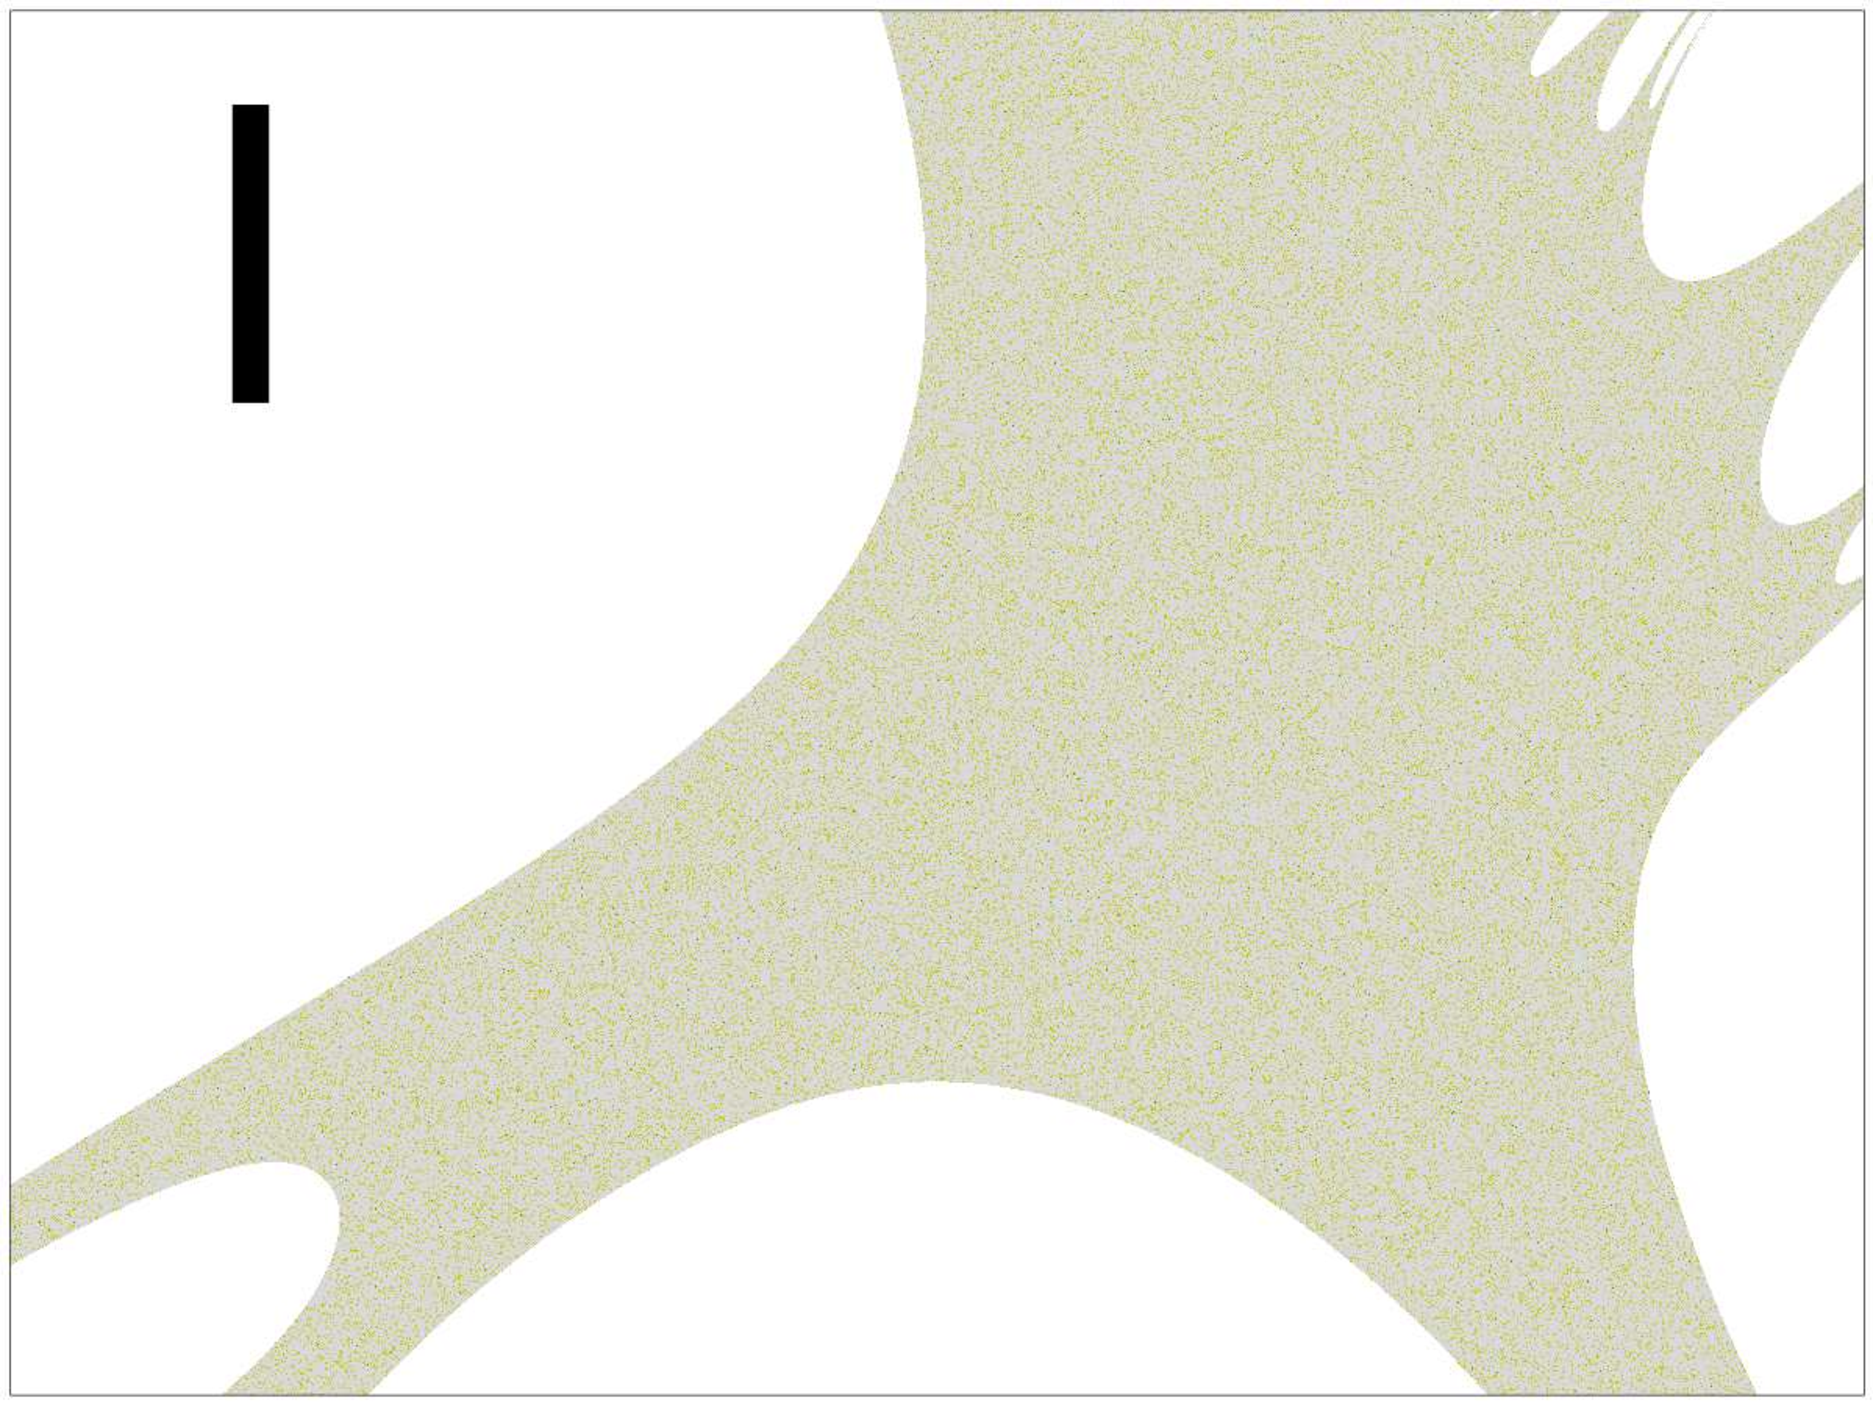
\includegraphics[width=0.35\textwidth]{m18}\\
\\   
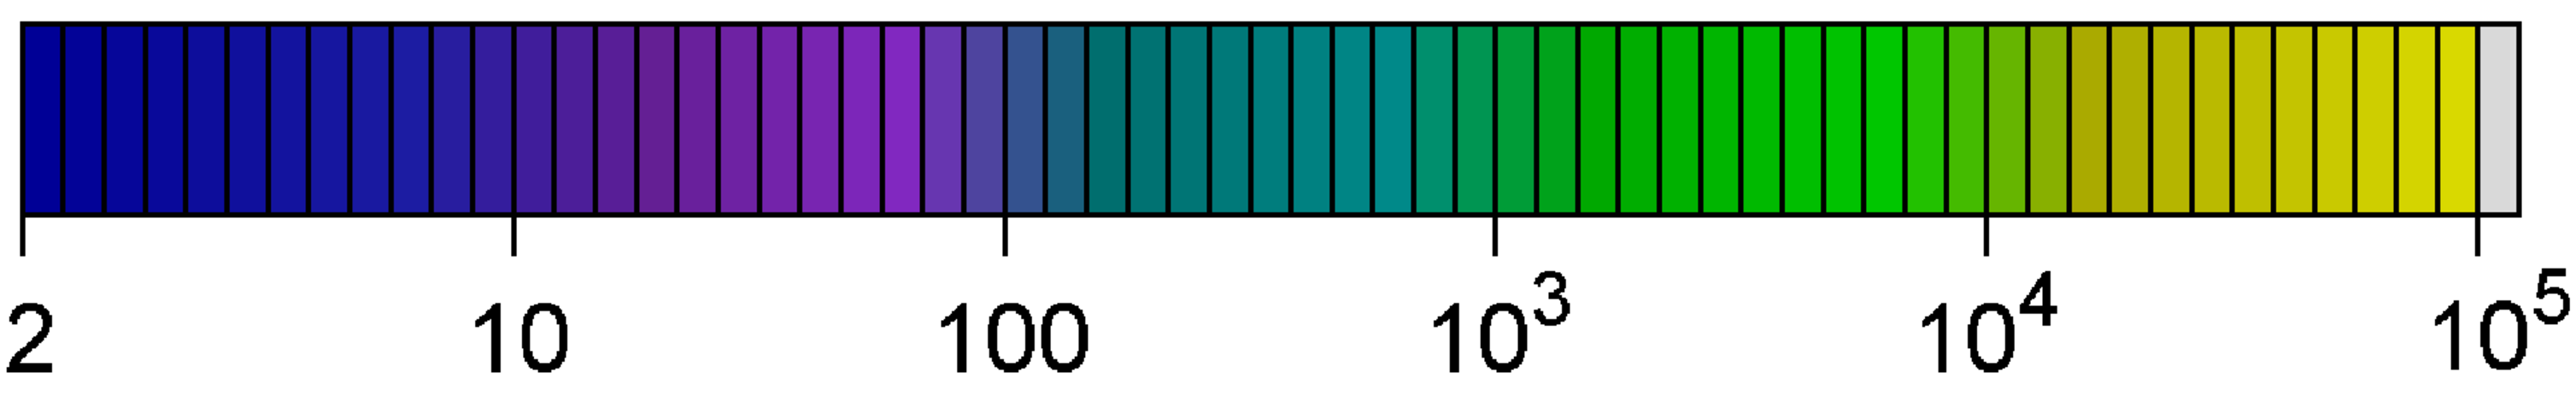
\includegraphics[width=0.6\textwidth]{ColorMapConEje}
\end{tabular}
\caption{Period's lengths evolution of the attraction domains for: (a) $n_f=5$, (b) $n_f=6$, (c) $n_f=7$, (d) $n_f=8$, (e) $n_f=9$, (f) $n_f=10$, (g) $n_f=11$, (h) $n_f=12$, (i) $n_f=13$, (j) $n_f=14$, (k) $n_f=17$, (l) $n_f=18$.}
\label{fig:m}
\end{figure*}

Fig. \ref{fig:m} shows that as the value of $n_f$ increases the colour of the area becomes more smooth and clear, indicating that the ICs converge to higher periods cycles. This is the range of initial values that generate useful sequences increases for higher values of $n_f$.

This can also be seen in Table \ref{tabla}, where as $n_f$ increases the predominant limit cycle's length increases.
In order to compare the obtained values with the real sequences we have simulated in floating-point with $236-$bit mantissa (IEEE $754$ octuple-precision binary floating-point format) we call this here \textit{floating-point} or just \textit{float}, it is the arithmetic closest to real numbers.
Then, using float precision all the limit cycles are higher than $10^5$, they converge to the chaotic attractor seen in Fig. \ref{fig:atractores3592}.d.

\begin{table*}[!t]
% increase table row spacing, adjust to taste
\renewcommand{\arraystretch}{1.3}
\caption{Lengths of the periods within the attractor domain $x$ and $y$ $\epsilon$  $[-2,2]$.}
\label{tabla}
\centering
\fontsize{9}{9}\selectfont
\begin{tabular}{l  l  }
\hline
$n_f$ & $T$ {\scriptsize(Percentage of ICs that converge to this period's length cycle)}  \\
\hline
\hline
$5$ & $2$ {\scriptsize($92.7\%$ )};$6$  {\scriptsize($7.3\% )$}\\
$6$ & $88$ {\scriptsize($41.6 \% )$};$44$ {\scriptsize($36.7 \% )$};$12$ {\scriptsize($13.8\% )$};$16$ {\scriptsize($6.2 \% )$};$2$ {\scriptsize($0.8 \% )$};$24$ {\scriptsize($0.6 \% )$};$26$ {\scriptsize($0.2 \%)$}\\
$7$ &  $12$ {\scriptsize($83.5 \% )$};$14$ {\scriptsize($8.9\% )$};$24$ {\scriptsize($5.2\% )$};$34$ {\scriptsize($1.8 \% )$};$2$ {\scriptsize($0.6\% )$} \\
$8$ & $68$ {\scriptsize($91.7\%)$};$14$ {\scriptsize($6.2\%)$};$12$ {\scriptsize($1.8 \%)$};$17$ {\scriptsize($0.2\% )$};$15$ {\scriptsize($0.1 \%)$}\\ 
$9$ & $140$ {\scriptsize($54.5 \%)$};$123$ {\scriptsize($25.4 \%)$};$34$ {\scriptsize($8.6\%)$};$44$ {\scriptsize($4.3 \%)$};$38$ {\scriptsize($3.9 \%)$};$22$ {\scriptsize($2.9 \%)$};$48$;$2$;$12$;$4$ {\scriptsize($<0.1\%)$}\\
$10$ & $655$ {\scriptsize($78.2\%)$};$212$ {\scriptsize($21.1\%)$};$143$ {\scriptsize($0.5\%)$};$12$ {\scriptsize($0.1\%)$};$2$;$36$;$13$;$20$;$10$;$4$ {\scriptsize($<0.1\%)$}\\
$11$ & $153$ {\scriptsize($78.1\%)$};$461$ {\scriptsize($10.8\% )$};$1381$ {\scriptsize($8.7\%)$};$434$ {\scriptsize($2.3\%)$};$18$;$30$;$53$;$32$;$34$;$10$;$2$ {\scriptsize($<0.1\% )$}\\
$12$ & $2,278$ {\scriptsize($64.4\%)$};$438$ {\scriptsize($22.4\% )$};$598$ {\scriptsize($7.6\% )$};$886$ {\scriptsize($4.7 \%)$};$12$ {\scriptsize($0.7\%)$};$87$;$2$;$42$;$23$;$32$;$10$ {\scriptsize($<0.1\% )$}\\
$13$ & $11,510$ {\scriptsize($ 98.9\%)$};$1052$ {\scriptsize($1 \%)$};$12$;$26$;$2$;$10$ {\scriptsize($<0.1\% )$}\\
$14$ & $21,333$ {\scriptsize($69.2\% )$};$5.804$ {\scriptsize($16.5\%  )$};$4,795$ {\scriptsize($7.9\%  )$};$1,264$ {\scriptsize($5.8 \% )$};$2,429$ {\scriptsize($0.5\% )$}\\ 
& $46$;$23$;$21$;$10$;$12$;$17$ {\scriptsize($<0.1\%  )$}\\ 
$15$ & $10,099$ {\scriptsize($58.6 \%)$};$1.762$ {\scriptsize($19.4 \%)$};$14,887$ {\scriptsize($18.3\%)$};$1,598$ {\scriptsize($3.4\%)$};$750$;$105$;$23$;$14$;$2$;$10$ {\scriptsize($<0.1\%)$}\\
$16$ & $54,718$ {\scriptsize($87.5\% )$};$5,017$ {\scriptsize($4.7\% )$};$>10^5$ {\scriptsize($3.7\% )$};$5,367$ {\scriptsize($2.5\% )$};$703$ {\scriptsize($0.9\% )$}\\
& $1,159$;$1,802$ {\scriptsize($0.2\% )$};$377$;$75$;$10$ {\scriptsize($<0.1\%  )$}\\  
$17$ & $37,812$ {\scriptsize($53.1\% )$};$38,456$ {\scriptsize($24.1\% )$};$>10^5$ {\scriptsize($16.0\%)$};$34,749$ {\scriptsize($3.0\% )$};$3,362$;$718$ {\scriptsize($1.5\%)$}\\
& $3,006$,$5,222$ {\scriptsize($0.1\% )$};$15$ {\scriptsize($<0.1 \%)$}\\  
$18$ & $>10^5$ {\scriptsize($87.4\%)$};$52,069$ {\scriptsize($12.5\% )$};$2,471$ {\scriptsize($0.1\% )$};$146$;$51$ {\scriptsize($<0.1 \%)$}\\
$float$ & $>10^5$ {\scriptsize($100\% )$}\\
\hline

\end{tabular}

\end{table*}


In relation to the randomness quantifiers, we realized that the analysis performed up to this point was not enough to fully describe the changes in the dynamic of a digitalized chaotic system.
To reach long periods does not ensure that the systems' exhibit good properties with respect to randomness. So we decided to further study the data obtained by employing statistical quantifiers.

As said, in Fig. \ref{fig:avvelo}.a the two gray zones correspond to the initial conditions that converge to the two coexisting cycles of period two and six respectively.
Then this two cycles will have a determined value of $H_{hist}$ and $H_{BP}$, $H_{hist}\mid_{T=2}=0.0625$, $H_{hist}\mid_{T=6}=0.1199$, $H_{BP}\mid_{T=2}=0.1053$ and $H_{BP}\mid_{T=6}=0.2723$.
However, the reported value of these quantifiers can not be the average of both, since the rate of occurrence of cycle two is much greater than that of cycle six (period two appears $92.7\%$ times while period six only $7.3\%$, see Table \ref{tabla}).
Therefore, we have calculated the averaged quantifiers by weighting each quantifier by its rate of occurrence.
%
\begin{figure}
    \centering
        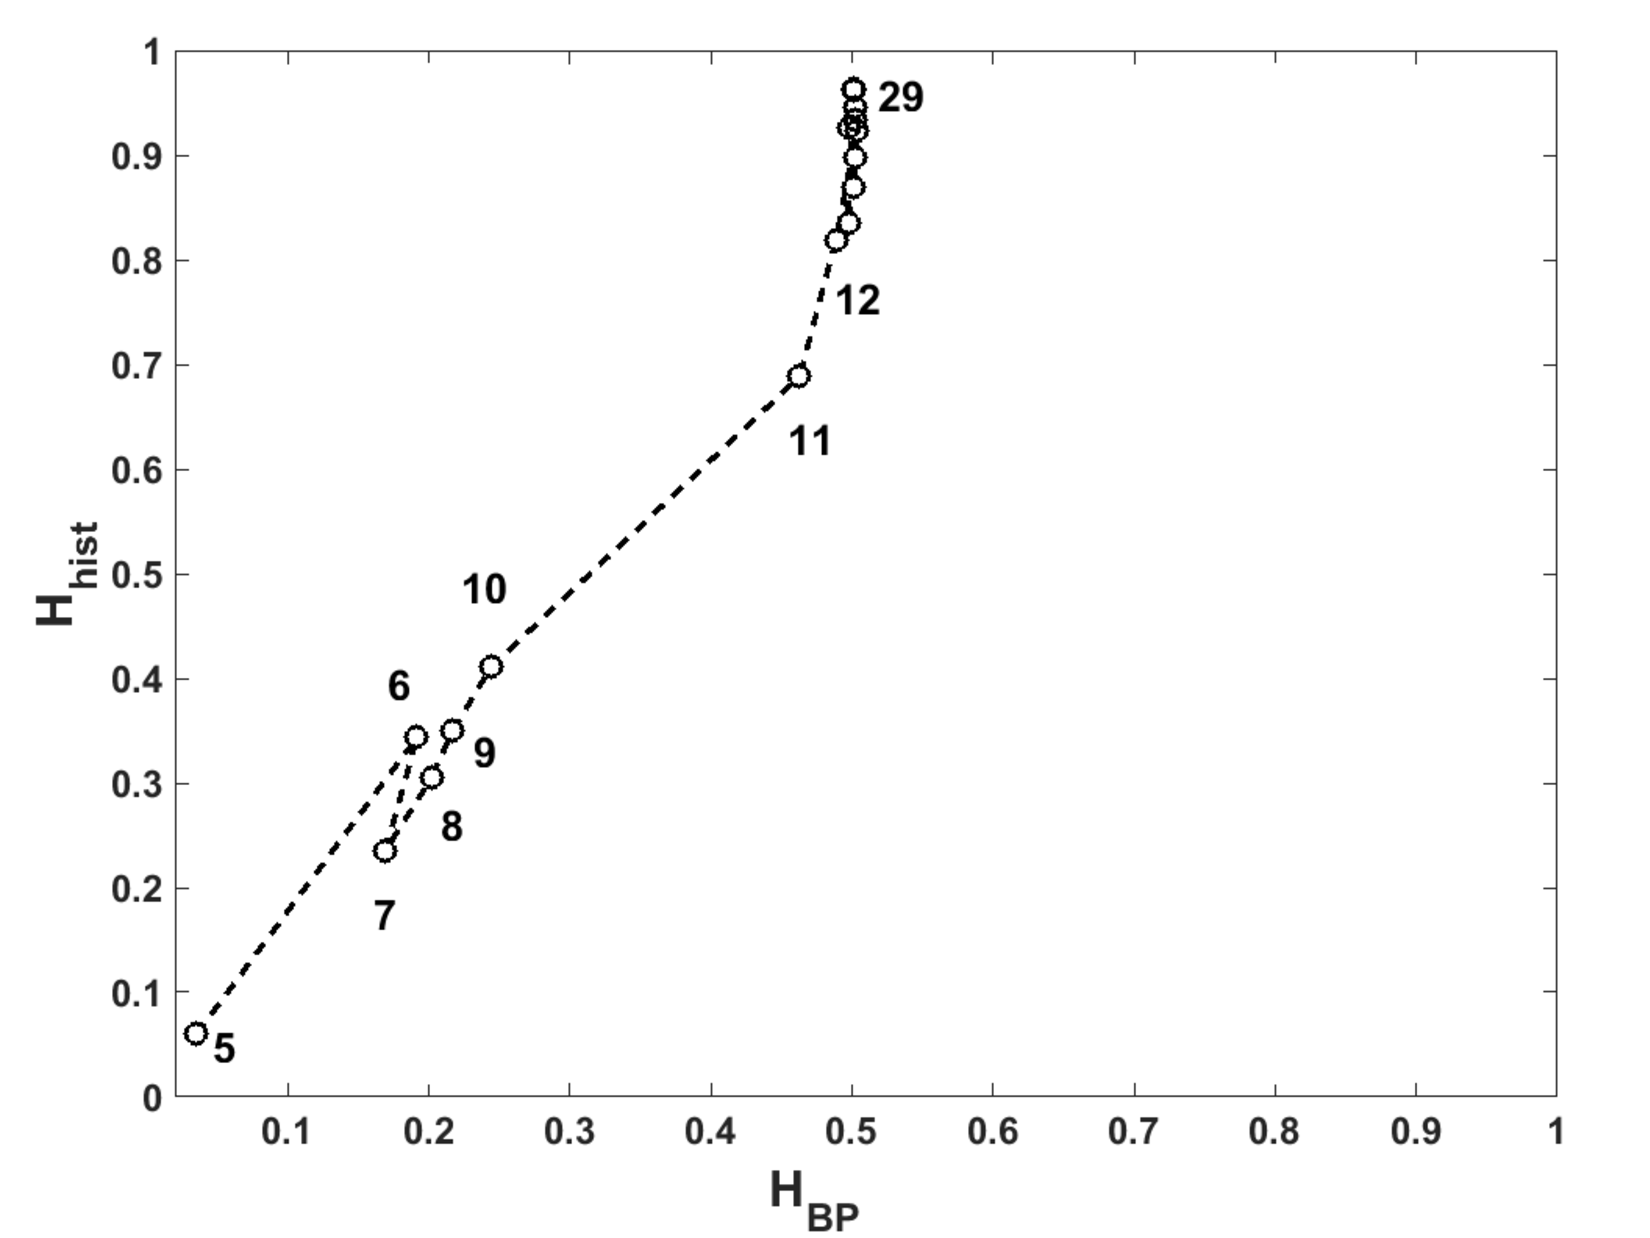
\includegraphics[width=0.85\columnwidth]{HBPvsHhistO}\\
    \caption{Plane $H_{hist}$ - $H_{BP}$  for different number of bits. }\label{fig:HBPvsHhist}
\end{figure}


The $H_{hist}$ vs $H_{BP}$ plane, shown in Fig. \ref{fig:HBPvsHhist}, allows a quick visualization of the behavior in terms of randomness of the system, in this plane the ``ideal" point, from the statistical point of view, is $(1,1)$.
Here, the system seems to stabilize for $n_f$ higher than $12$.
It can be seen that while the $H_{hist}$ stabilizes close to the maximum value ($H_{hist}=1$), the $H_{BP}$ tends to stabilizes to $0.5$.
This value of $H_{BP}$ is characteristic of chaotic systems and is due to the inner structures of their attractors.

A summary of the observed analysis of these outputs can be seen in Fig. \ref{puntos}.
%
\begin{figure}
    \centering
    \begin{subfigure}[b]{0.49\textwidth}
        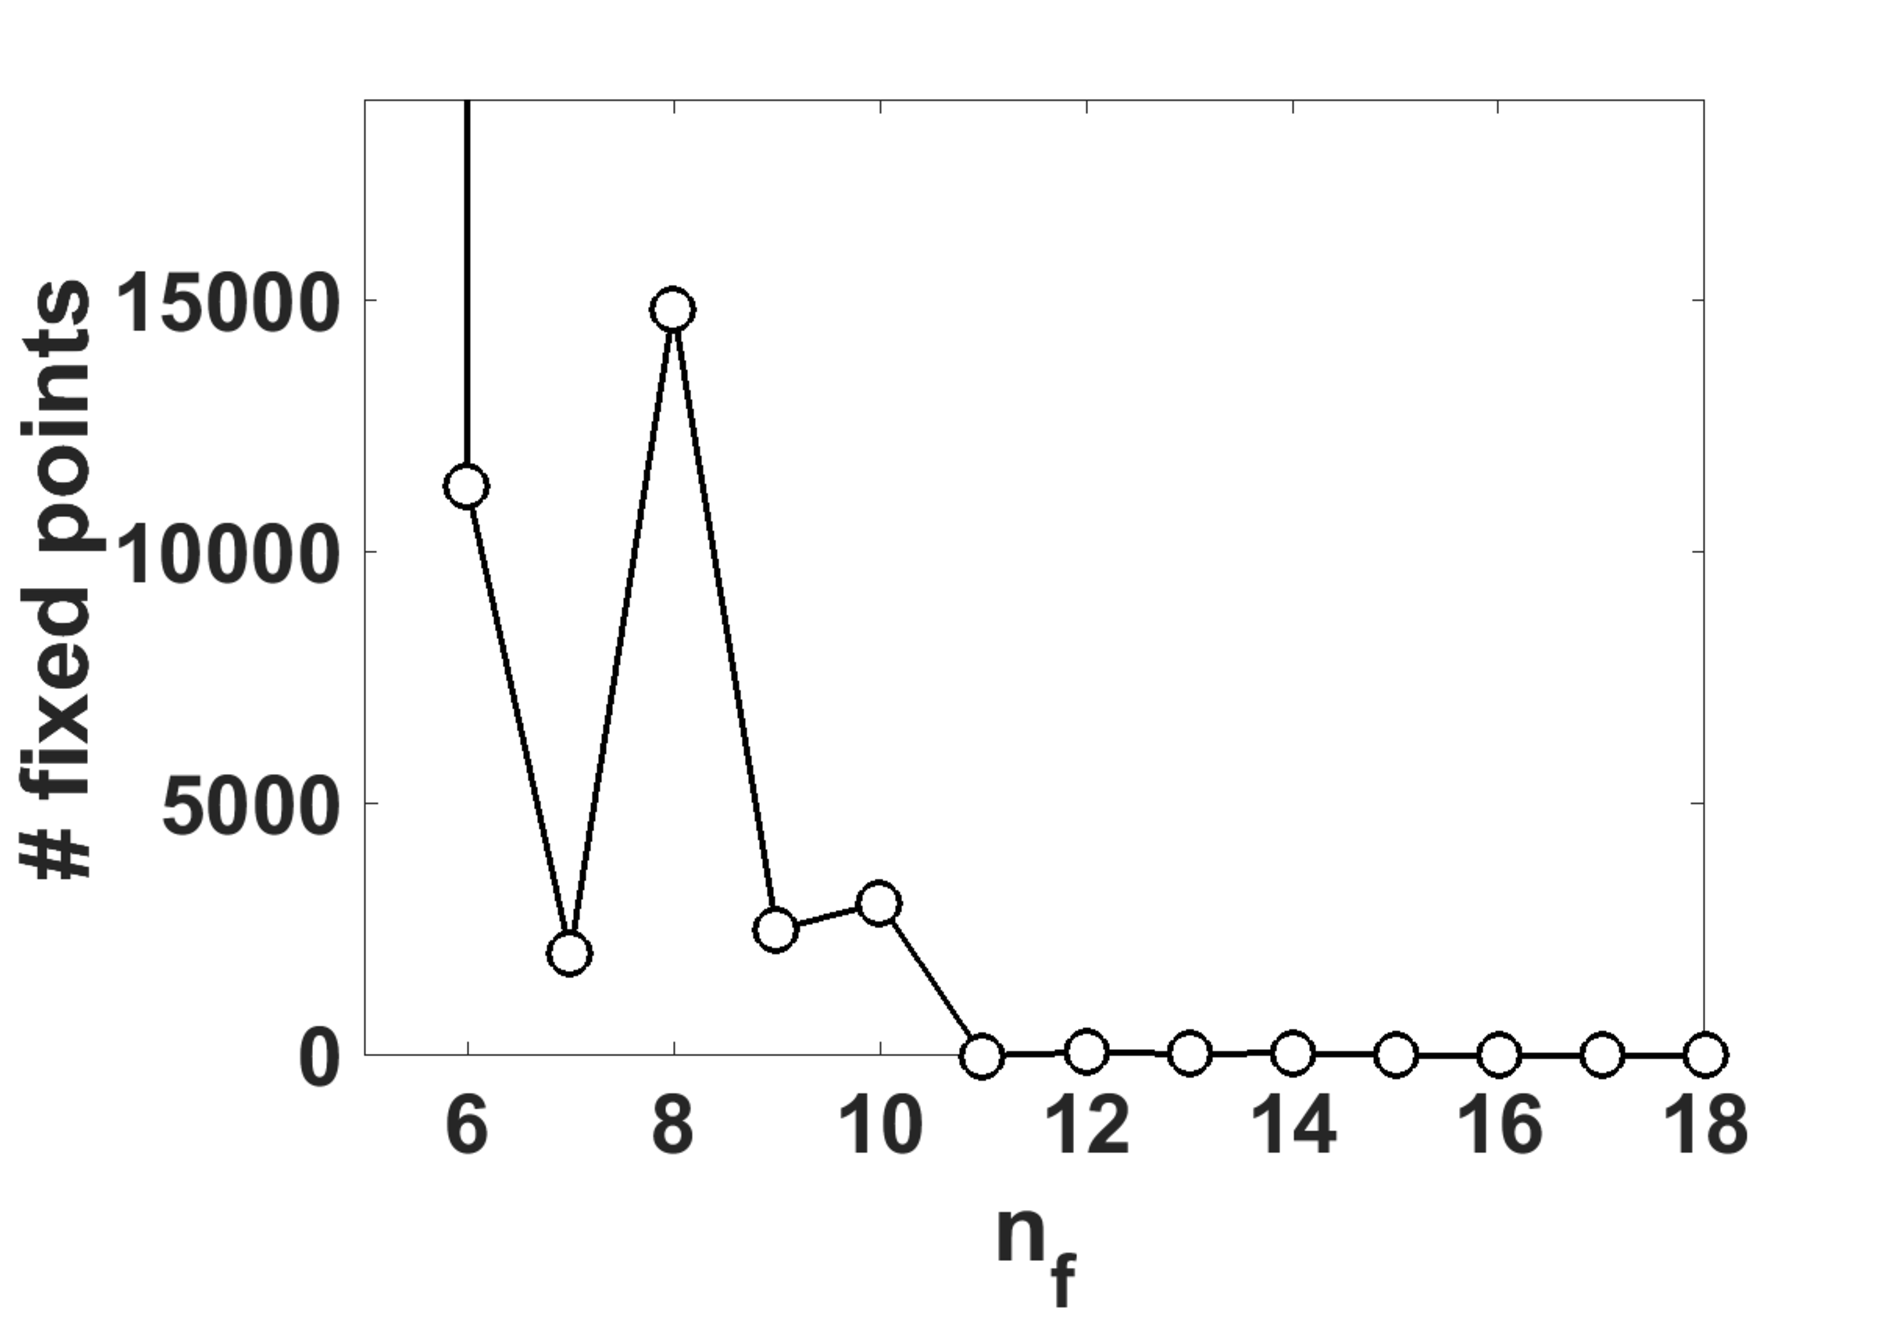
\includegraphics[width=\textwidth]{ptosfijosO}
        \caption{number of fixed points.}
        \label{fig:gull}
    \end{subfigure}
    \hfill 
    \begin{subfigure}[b]{0.49\textwidth}
        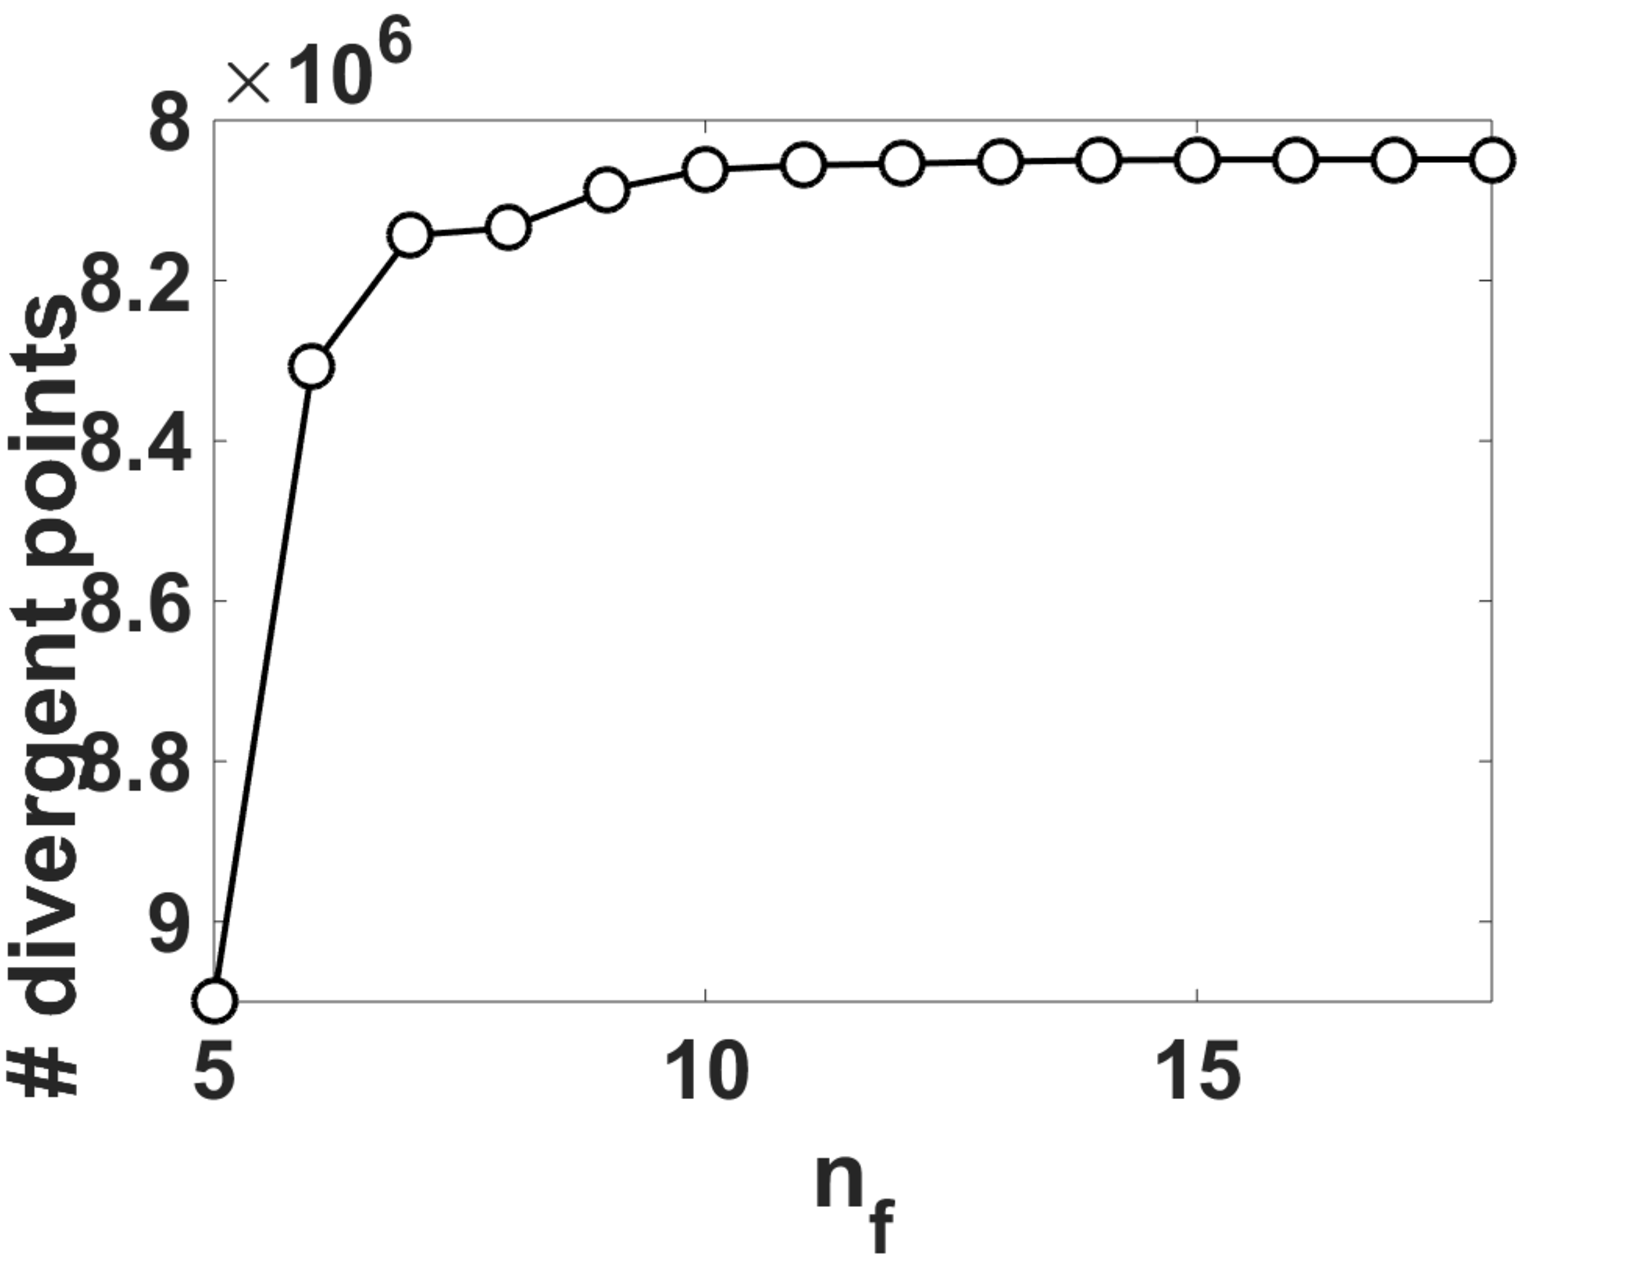
\includegraphics[width=\textwidth]{divergenO}
        \caption{number of divergent points.}
        \label{fig:tiger}
    \end{subfigure}
   \hfill 
    \begin{subfigure}[b]{0.49\textwidth}
        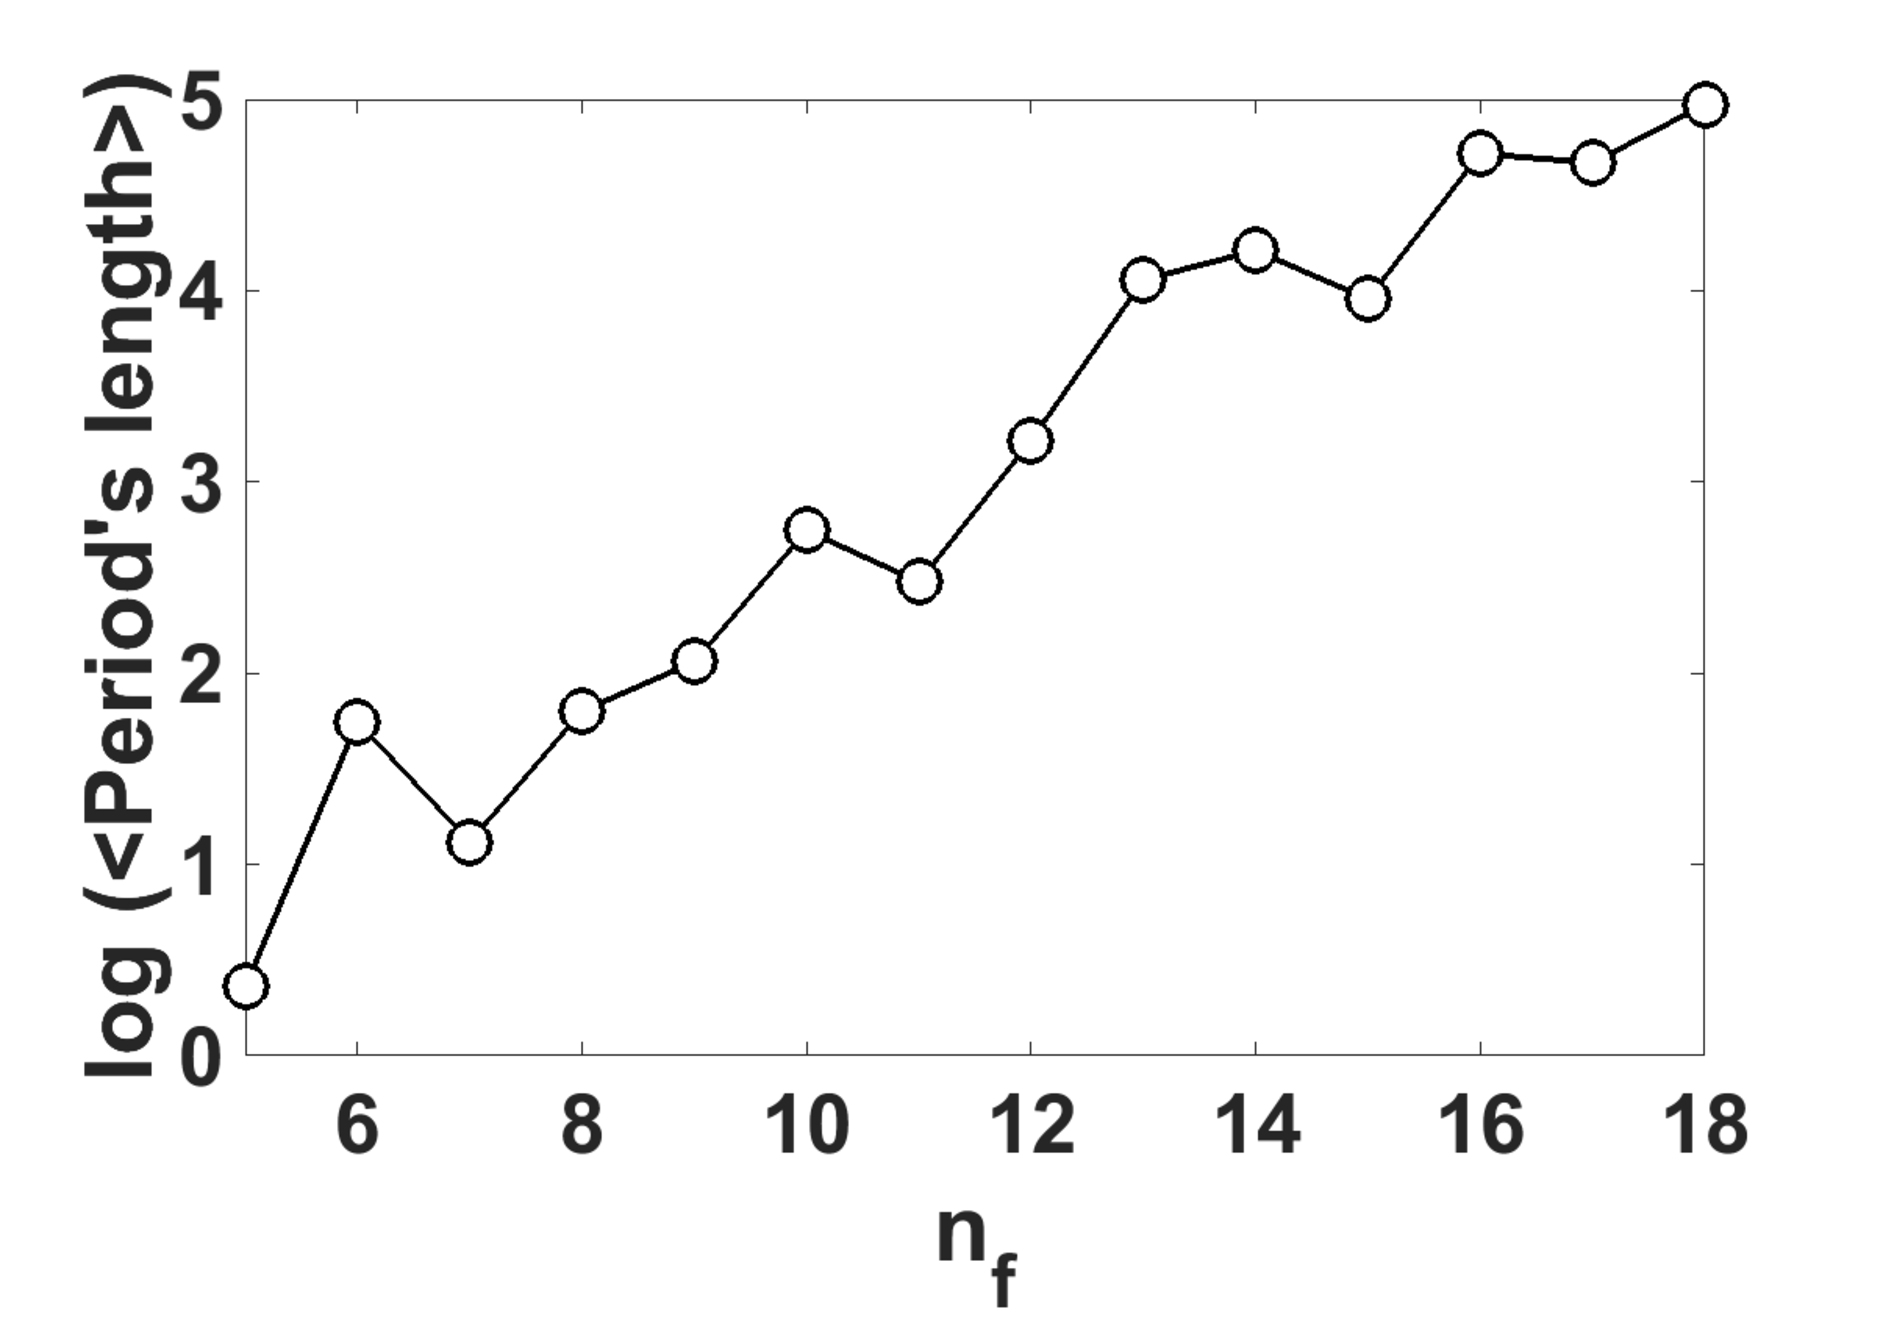
\includegraphics[width=\textwidth]{Periodos_promO}
        \caption{logarithm of the length's cycles weighted average.}
        \label{fig:mouse}
    \end{subfigure}
  \hfill   
    \begin{subfigure}[b]{0.49\textwidth}
        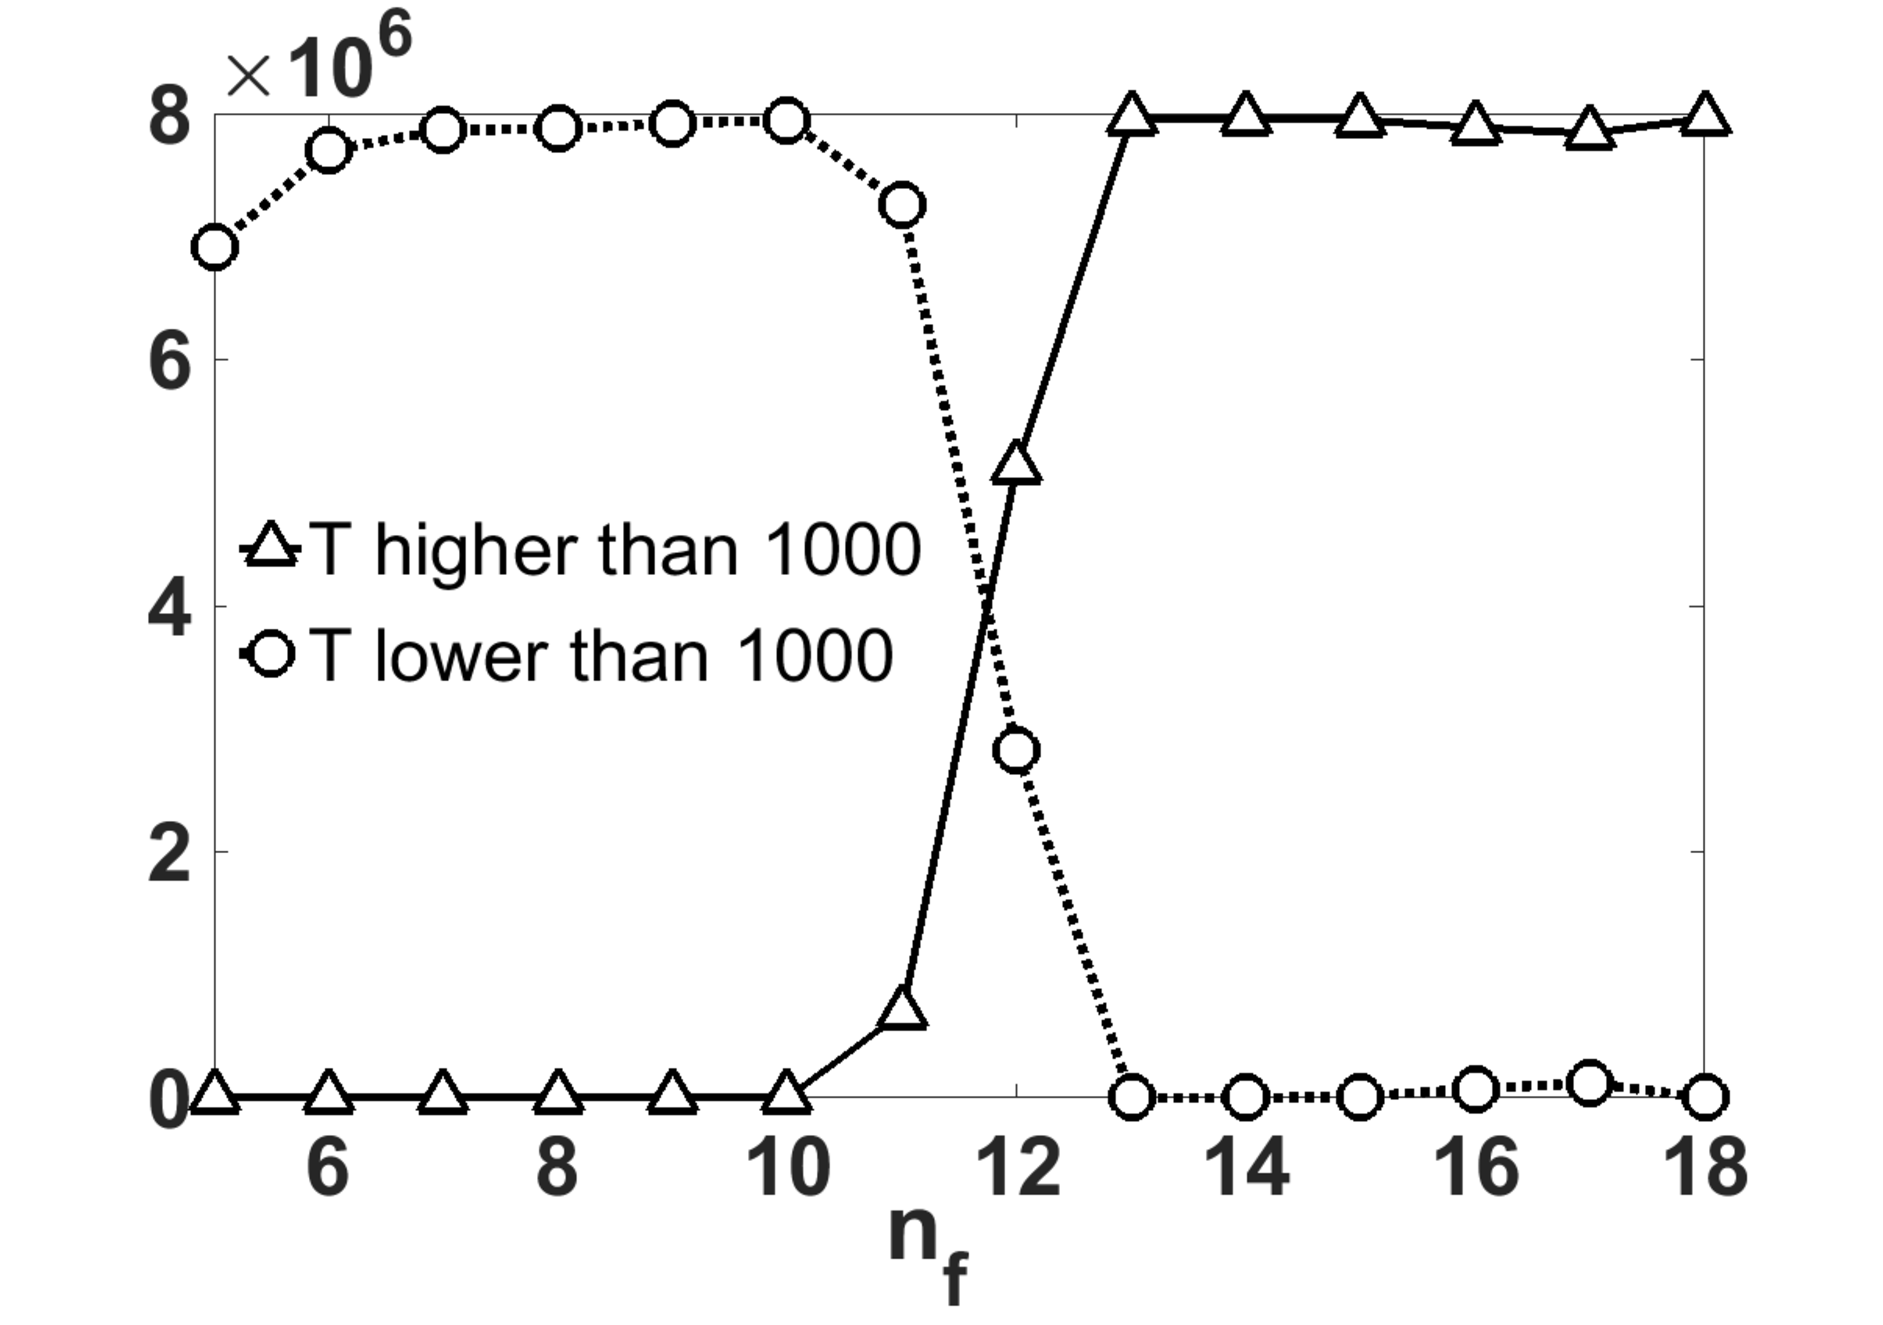
\includegraphics[width=\textwidth]{PuntosO}
        \caption{initial conditions with period length higher and lower than $1,000$.}
        \label{fig:mouse}
    \end{subfigure}
    \caption{Summary of initial conditions' behavior.}\label{puntos}
\end{figure}


Fig. \ref{puntos}.a and \ref{puntos}.b show the number of points that diverge and converge to fixed points respectively as the value of $n_f$ increases, in both cases, the final value tends to the floating-point case.
It is clear from these figures that for $n_f \sim 12$ the system seems to have stabilized.
Figure \ref{puntos}.c shows that the averaged period of cycles increases at a logarithmic rate.
Finally, Fig. \ref{puntos}.d shows the number of initial conditions that present periods $T$ higher and lower than $1,000$.
Again, a value of $12$ for $n_f$ seems to be the limit to obtain a good approximation of the system.

Figure \ref{fig:HBPHhist} shows the weighted average of quantifiers $H_{hist}$, $H_{BP}$ and \textsl{MLE}.
In the figure it can be seen that the three quantifiers tend to the value calculated using floating-point arithmetic.
While $H_{BP}$ and \textsl{MLE} stabilize for $n_f \sim 12$ or $13$, $H_{hist}$ reaches the floating-point value for $n_f \sim 19$, showing that there are properties of the output sequences that only this quantifier can detect.
This confirms the need to use both quantifiers to characterize the randomness of the sequences.
%
\begin{figure}
    \centering
        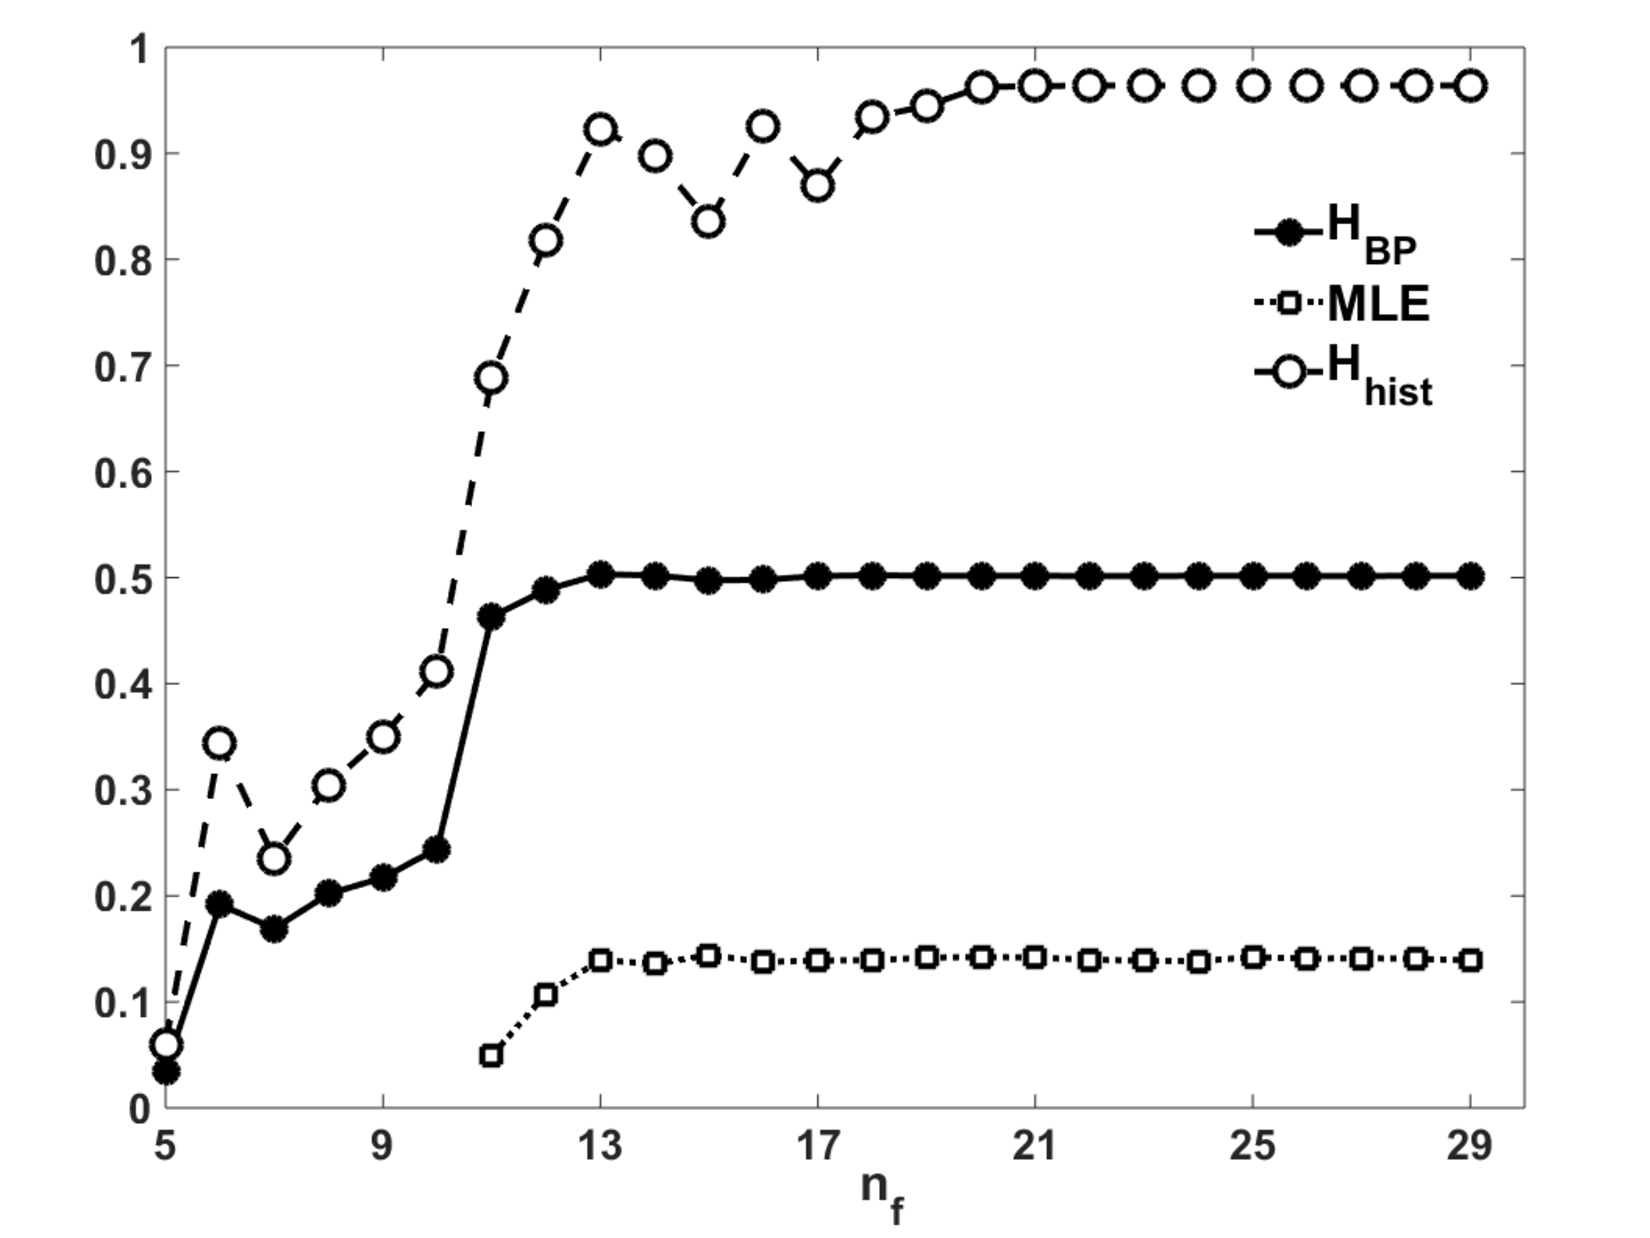
\includegraphics[width=0.75\columnwidth]{HBPHhistO}\\
    \caption{Weighted average of quantifiers $H_{BP}$,  $H_{hist}$ and \textsl{MLE} as functions of the number of bits.}\label{fig:HBPHhist}
\end{figure}

As can be seen from the above analysis, the minimum number of bits is determined by $H_{hist}$ quantifier and results to be $n_f=19$ plus the number of bits used to represent the integer part $n_i=4$, therefore $n_{min}$ turns out to be equal to $23$.